%#!make thesis.dvi
\documentclass[platex,a4paper,report,12pt,dvipdfmx]{jsbook}
%\documentclass[draft,a4paper,report,12pt]{jsbook}
% 執筆中はdraft↑を入れた方が速い
%\documentclass[english,draft,a4paper,report,12pt]{jsbook}
% ↑for English writing

%% amsmathを使う場合はthesisより前に読み込む
\usepackage{amsmath}
\usepackage{amssymb, amsmath}
\usepackage{thesis}
\usepackage{mediabb}
%\usepackage{newenum}
%\usepackage{epsfig}
%\usepackage{listings}
%\usepackage{url}
%\usepackage{fancyhdr}
% \usepackage{subfigure}
%\usepackage[dvipdfm]{graphicx}
\usepackage{cite}
\usepackage{bm}
\usepackage{afterpage}
%\usepackage{wrapfig}
\usepackage{caption}
\usepackage{subcaption}
\usepackage{multirow}
\usepackage {colortbl,array,xcolor}
\usepackage{url}

\usepackage{algorithm}
\usepackage{algpseudocode}
\usepackage{float} % figureの[H]指定を使う

%------------------------------
%\hyperref
%  日本語の文字コード設定が分からない人はコメントアウトすること.
%------------------------------
% PDF化したときにしおりが作成され,図表へのジャンプも可能となる.
%\usepackage{atbegshi}
% Mac/Linuxの場合

%   ※Ubuntuの場合はEUC-UCS2を自分で入れないとダメ.
%\AtBeginShipotutFirst{\special{pdf:tounicode EUC-UCS2}}
%% Winの場合
%\AtBeginShipoutFirst{\special{pdf:tounicode 90ms-RKSJ-UCS2}}
% 以下は共通
\usepackage{comment}
\usepackage{fancyhdr}
\usepackage[a4paper,bookmarks,bookmarksnumbered,%
 bookmarksopen=false,pdfstartview={FitH},%
 bookmarkstype=toc,%
 setpagesize=false,%
 pdfauthor={37-246529 },%
 pdftitle={thesis}]{hyperref}

%----------------------------------------------------------------------
% 設定
%----------------------------------------------------------------------
% 設定ファイルの読み込み
%!make thesis.dvi
%======================================================================
% $B@_Dj(B
%======================================================================

%----------------------------------------------------------------------
% $B>O!$@a$J$I(B
%----------------------------------------------------------------------
\def\thesection{\arabic{chapter}.\arabic{section}}
\def\thesubsection{\arabic{chapter}.\arabic{section}.\arabic{subsection}}
\def\thesubsubsection{(\alph{subsubsection})}
\def\theenumii{\roman{enumii}}
\def\labelenumii{(\theenumii)}

%----------------------------------------------------------------------
% $B?t<0(B
%----------------------------------------------------------------------
% Equation
%\makeatletter
%\def\theequation{%
% \arabic{section}.\arabic{equation}}
%\@addtoreset{equation}{section}
%\makeatother

%----------------------------------------------------------------------
% Caption
%----------------------------------------------------------------------
\makeatletter
\long\def\@makecaption#1#2{
  \vskip\abovecaptionskip
  \iftdir\sbox\@tempboxa{#1\hskip1zw#2}
    \else\sbox\@tempboxa{#1\ \ #2}
  \fi
  \ifdim \wd\@tempboxa >\hsize%
    \iftdir #1\hskip1zw#2\relax\par
      \else #1\ \ #2\relax\par\fi
  \else
    \global \@minipagefalse
    \hbox to\hsize{\hfil\box\@tempboxa\hfil}
  \fi
  \vskip\belowcaptionskip}
\makeatother


%----------------------------------------------------------------------
% enumerate$B4D6-(B
%----------------------------------------------------------------------
% enum$B$N=q<0JQ99(B
\makeatletter
\renewcommand{\theenumi}{\@arabic\c@enumi}
\renewcommand{\labelenumi}{\kern-.5zw $B!J(B\,\theenumi\,$B!K(B\kern-.5zw}

% enumerate$B4D6-$N%$%s%G%s%H$rJQ99(B
\renewenvironment{enumerate}
  {%
   \ifnum \@enumdepth >3\relax\@toodeep\else
    \advance\@enumdepth\@ne
    \edef\@enumctr{enum\romannumeral\the\@enumdepth}%
    \list{\csname label\@enumctr\endcsname}{%
    \leftmargin1.5zw
    \labelsep1zw
    \labelwidth\z@
    \itemindent2zw
    \listparindent1zw
    \topsep\z@\parsep\z@\partopsep\z@\itemsep\z@
    \usecounter{\@enumctr}%
    \def\makelabel##1{\hss\llap{##1}}}%
   \fi}{\endlist}
\makeatother


%----------------------------------------------------------------------
% hyperref-dvipdfm$B$N=$@5(B
%   OSX$B$N(BPreview.app$B$G$A$c$s$HF0$/$h$&$K$9$kBP:v(B
%----------------------------------------------------------------------
\makeatletter
\def\@pdfm@dest#1{%
  \Hy@SaveLastskip
  \@pdfm@mark{dest (#1) [@thispage /\@pdfview\space @xpos @ypos null]}%
  \Hy@RestoreLastskip
  }
\makeatother


%\rhead{\leftmark}

%----------------------------------------------------------------------
% $B!V;29MJ88%!W$rL\<!$K=P$9(B
%----------------------------------------------------------------------
% \makeatletter%% $B%W%j%"%s%V%k$GDj5A$9$k>l9g$OI,?\(B
%% (j)report$B!&(B(j)book $B%/%i%9$N>l9g(B
%%
% \renewenvironment{thebibliography}[1]% $B:FDj5A(B
% {\chapter*{\bibname\@mkboth{\bibname}{\bibname}}%
%  \addcontentsline{toc}{chapter}{\bibname}% $B$3$N9TDI2C(B
%    \list{\@biblabel{\@arabic\c@enumiv}}%
%         {\settowidth\labelwidth{\@biblabel{#1}}%
%          \leftmargin\labelwidth
%          \advance\leftmargin\labelsep
%          \@openbib@code
%          \usecounter{enumiv}%
%          \let\p@enumiv\@empty
%          \renewcommand\theenumiv{\@arabic\c@enumiv}}%
%    \sloppy
%    \clubpenalty4000
%    \@clubpenalty\clubpenalty
%    \widowpenalty4000%
%    \sfcode`\.\@m}
%   {\def\@noitemerr
%     {\@latex@warning{Empty `thebibliography' environment}}%
%    \endlist}

%%
% \def\chaptermark#1{\markboth {\ifnum \c@secnumdepth>\m@ne
% \@chapapp\ \thechapter \@chappos\ \fi #1}{}}
% \makeatother%% $B%W%j%"%s%V%k$GDj5A$9$k>l9g$OI,?\(B

% マクロファイルの読み込み
%======================================================================
% Macros
%======================================================================

%----------------------------------------------------------------------
% $BI=$G;H$&B@$a$N7S@~(B: \Hline
%----------------------------------------------------------------------
% IEICE Trans.$B$+$i$N%Q%/%j(B
% $BL$Dj5A$N;~$@$1Dj5A(B
\makeatletter
 \@ifundefined{Hline}{\newcommand{\Hline}{\noalign{\hrule height 0.4mm}}}
\makeatother


%----------------------------------------------------------------------
% desclab$B4D6-(B
%----------------------------------------------------------------------
% $B;H$$J}(B 
% \begin{desclab}{$B%i%Y%k$,0lHVD9$$$d$D(B}
%  \item[$B%i%Y%k(B1] $B$[$2!<(B
%  \item[$B%i%Y%k(B2] $B$U$,!<(B
%  \item[$B%i%Y%k(B3] $B$U$,$U$,(B
% \end{desclab}
\def\desclablabel#1{\bf #1\hfill}
\def\desclab#1{\list{}%
 {\settowidth{\labelwidth}{\desclablabel{#1}}
 \leftmargin\labelwidth
 \advance\leftmargin\labelsep}
 \let\makelabel\desclablabel}
\let\enddesclab\endlist


%----------------------------------------------------------------------
% $B?t;z$K%+%s%^$rIU2C!??t;z$+$i%+%s%^$r:o=|(B
%----------------------------------------------------------------------
% $B$3$3$+$iGR<Z(B
%   http://mytexpert.sourceforge.jp/index.php?%A5%E1%A5%E2%C4%A2%2FTeX%A5%DE%A5%AF%A5%ED3
% $B;H$$J}(B
%   \appendComma{10000}
%   \stripComma{10,000}
\makeatletter
\newcount\@cnt@apcma
\newcount\@cnt@apcmc
%------------------------------
% $B%+%s%^$r<h$j=|$/(B
\def\strip@comma#1{%
  \def\@tempstr{,}%
  \expandafter\@tfor \expandafter\member
   \expandafter:\expandafter=#1\expandafter\do{%
     % $B$b$7%+%s%^$J$i<N$F$k!"$=$l0J30$OI=<((B
     \ifx\member\@tempstr\else\member\fi
   }%
}
%------------------------------
% $B%+%s%^$rDI2C$9$k(B
\def \append@comma#1{%
  \def \@tempstr {,}%
  \let \@temp@reversed \@empty
  \expandafter\@tfor \expandafter\member
  \expandafter:\expandafter=#1\expandafter\do{%
    % $B$^$:$OA4$F$NMWAG$r5UE>$5$;$k(B
    \edef \@temp@reversed {\member \@temp@reversed}%
  }%
  \@cnt@apcma \z@
  \let \@temp@appended \@empty
  \expandafter\@tfor \expandafter\member
  \expandafter:\expandafter=\@temp@reversed \expandafter\do{%
    % $B;M$DL\$NMWAG$N>l9g$O(B {0000} $B$H$J$C$F$$$k$N$r(B car $B$H(B cdr $B$G(B
    %   \@tempcmda := car (\@temp@appended) [$B@hF,(B]
    %   \@tempcmdb := cdr (\@temp@appended) [$B@hF,0J30(B]
    % $B$K$7$F(B {[$B@hF,(B],[$B@hF,0J30(B]}$B$H$$$&=hM}$,$G$-$k$h$&$KA0=hM}!%(B
    % $B$3$3$G(B \@temp@appended $B$K(B \member $B$rDI2C!J(B\member $B$,6u$N;~$b(B
    % $B$"$k!K!%(B
    %    \@temp@appended := {\member \@tempcmda,\@tempcmdb}
    \ifnum \@cnt@apcma = 4
      \edef \@tempcmda {\expandafter \@car \@temp@appended \@nil}%
      \edef \@tempcmdb {\expandafter \@cdr \@temp@appended \@nil}%
      \edef \@temp@appended {\member \@tempcmda,\@tempcmdb}%
      %o(\the\@cnt@apcma-\@tempcmda:\@tempcmdb)o% for debug
      % $B$3$3$G%+%&%s%?$r<!$N%+%s%^$N$?$a$K(B 1 $B$K@_Dj$9$k(B
      % $B$3$NJ,4t$K$$$k;~E@$G(B $5i (i = 0, 1, \ldots, k)$ $BHVL\$N$?$a!%(B
      \@cnt@apcma \@ne 
    \else
      % 4$BHVL\$G$O$J$$MWAG$N>l9g$O$=$N$^$^(B \member $B$r%j%9%H$KDI2C(B
      % \@temp@appended := {\member \@temp@appended}
      \edef \@temp@appended {\member \@temp@appended}%
    \fi
    \advance \@cnt@apcma \@ne
  }%
  % $B:G4|$K%j%9%H$rI=<($9$k(B
  \@temp@appended 
}
% 
\let \stripComma \strip@comma
\let \appendComma \append@comma
\makeatother

\pagestyle{footandheadings}
\pagenumbering{roman}
\setcounter{tocdepth}{3}

% 目次の深さはsubsectionまで
\setcounter{tocdepth}{2}

%ここでページのヘッダーを編集
\pagestyle{fancy}
\lhead{\rightmark}
\cfoot{\thepage}
\setlength{\headheight}{16pt}
\renewcommand{\chaptermark}[1]{\markboth{第\  \normalfont\thechapter\ 章~~#1}{}}
\renewcommand{\sectionmark}[1]{\markright{\thesection #1}{}}
\lhead{}
\newcommand{\bs}{\symbol{'134}}
\newcommand{\Cmd}[1]{\texttt{\def\{{\char`\{}\def\}{\char`\}}\bs#1}}

\pagenumbering{roman}

% 基準となる図の幅
\newlength\figurewidth
\setlength{\figurewidth}{0.8\textwidth}
% 縦に並べた図の間の基準となるスペース
\newlength\figuresep
\setlength{\figuresep}{0.3\floatsep}


%----------------------------------------------------------------------
% タイトル
%----------------------------------------------------------------------
\title{\huge 時系列補間型学習データに基づく疎パイロット下の無線チャネル予測機構
}
\subtitle{}

\ID{37-246529}
\author{松橋 悠}
\professor{森川 博之 教授}
\professorii{}
\faculty{東京大学大学院工学系研究科}
\department{電気系工学専攻}
\date{2025年1月22日}


% ↓includeonlyを活用すると処理が速いので書いてる途中はお勧め.
% \includeonly{1st,2nd, acknowledge}

%----------------------------------------------------------------------
% 本文
%----------------------------------------------------------------------
\begin{document}
%#!make thesis.dvi
%======================================================================
% タイトル
%======================================================================
\maketitle
\setcounter{page}{0}
\newpage
\tableofcontents
\listoffigures
\listoftables
\clearpage

\pagenumbering{arabic}
\newpage
\renewcommand{\baselinestretch}{1}


%----------------------------------------------------------------------
% 中身
%----------------------------------------------------------------------
%序論
%#!make thesis.dvi
%======================================================================
% 序論
%======================================================================
\chapter{序論}{}
\label{chap:1st}

\section{本論文の背景と目的}

% ステップ①:社会的・技術的な大背景の提示
5G以降の移動体通信では,高周波数帯の利用と大規模MIMO技術の導入が進んでいる.
基地局は多数のアンテナ素子を用いてビームフォーミングやプリコーディングを行い,空間多重により通信容量を確保する.
これらの送信処理では,送受信間の伝搬特性を表すチャネル状態情報が不可欠である.
チャネル状態情報の誤差はビームの指向ずれや干渉増大を招き,通信品質の劣化に直結する.

チャネル状態情報は,端末が送信する参照信号に基づいて基地局が推定する.
アンテナ素子数や同時接続ユーザ数が増加すると,チャネル状態情報の次元と更新頻度の要求が増大する.
参照信号の送信頻度を高めれば推定精度は向上するが,時間周波数リソースと送信電力を消費し,データ伝送に割ける資源を圧迫する.
加えて,移動や遮蔽物によりチャネルが時間変動する環境では,推定から利用までの遅延によりチャネル状態情報が陳腐化するチャネルエイジングが問題となる.
以上より,チャネル状態情報の推定精度と更新コストの両立が課題となっている.

% ステップ②:解決策(キー技術)の導入とメリット
参照信号のオーバーヘッドを抑えつつ将来のチャネル状態情報を推定する手段として,時系列CSI予測が研究されている.
時系列CSI予測は,過去の観測系列から将来時刻のチャネル状態情報を外挿する枠組みである.
予測値をビームフォーミングやプリコーディングに用いれば,参照信号の送信頻度を低減しながら通信品質を維持できる.
近年は深層学習を用いてチャネルの時間変動をデータから学習する手法が提案されており,古典的なウィナーフィルタやカルマンフィルタに比べて柔軟なモデル化が期待できる.

% ステップ③:研究課題の具体化
時系列CSI予測を実環境で運用するには,学習時と異なる環境への適応が求められる.
基地局配置,周波数帯,散乱特性,移動速度が変化すると,訓練分布とテスト分布が不一致となり,予測誤差が増大する.
セル内の建造物の増減や時間帯に伴うユーザ密度の変化も,電波伝搬環境を変化させる要因となる.
このような分布変化に追従するには,運用中にモデルを更新する仕組みが必要である.

既存のモデル更新手法の多くは,新環境で得られる正解データを用いた教師あり学習を前提としている.
一方,時系列CSI予測で参照信号を削減する場合,予測スロットでは参照信号を送信しないため,予測対象時刻のチャネル状態情報を観測できない.
正解ラベルが欠損する状況では,予測値と真値の誤差を計算できず,教師あり学習に基づくモデル更新が困難となる.
予測を一時停止して参照信号を送信すれば正解ラベルを取得できるが,参照信号削減という時系列CSI予測の目的に反する.
以上より,参照信号削減を維持しながら予測モデルを更新する枠組みが必要である.

% ステップ④:本研究の目的と貢献(提案手法)
本研究では,参照信号削減下において予測を継続しながら時系列CSI予測モデルを更新する機構を提案する.
提案機構の要点は,欠損した正解ラベルを補間により事後的に推定し,補間値を含む系列から更新用の学習サンプルを構成する点にある.
予測スロットより後に得られる観測値を用いて補間値を算出するため,参照信号削減を維持したまま学習サンプルを生成できる.
本論文では,複数の補間手法を比較して有効な手法を選定し,提案機構の有効性をシミュレーションにより検証する.
評価シナリオとして,新規基地局への展開とセル内の環境変動を想定し,いずれの場合においても予測精度が改善することを示す.


% NOTE: 参照先画像が存在しないためコメントアウト(ビルドエラー回避)
% \begin{figure}[htbp]
%   \centering
%   \includegraphics[width=0.8\linewidth]{img/2nd/test.png.pdf}
%   \caption{テスト画像の挿入}
%   \label{fig:test_image}
% \end{figure}

\section{本論文の構成}

\noindent
本論文は全5章で構成される.
第1章では,本研究の背景と目的を述べる.
第2章では,5G NR物理層における無線伝搬とCSI取得の枠組みを整理し,時系列CSI予測が必要となる背景と関連研究,および環境適応における課題を述べる.
第3章では,参照信号削減に伴い欠損するCSIを扱うための時系列補間手法を定式化し,レイトレーシングにより生成したCSI系列を用いて補間精度を比較する.
第4章では,補間値に基づき更新用サンプルを構成して予測モデルを更新する機構を提案し,複数のシナリオで有効性を評価する.
第5章では,本研究で得られた知見をまとめ,今後の課題を述べる.

% 背景, 先行研究
\chapter{5G NR物理層におけるチャネル予測}{}
\label{chap:2nd}
%★名言が必要ない場合には空っぽにすればOK.

\section{はじめに}
本章ではMIMO(Multiple-Input Multiple-Output)伝送を扱うために必要な基礎事項を整理する.
まずチャネルの表現を帯域幅とアンテナ数の観点から整理し,狭域・広域,SISO・MIMOの違いを明確にする.
続いて,本論文で用いる前提(広域MIMOの周波数領域表現)を定義する.



\section{5G NRの物理層における無線伝送処理}



移動体通信におけるチャネルは,送信信号が空間を伝搬して受信信号へ至る対応関係を表す.
無線信号は搬送波による周波数変換を経て送受信されるため,解析では一般に複素ベースバンド表現を用いる.
複素ベースバンド信号とは,送信側では変調後に搬送波へ上変換する直前,受信側では搬送波から下変換した直後で復調する前の,I成分およびQ成分で表される複素信号である.

本節では,帯域幅とアンテナ数の観点からチャネルモデルを整理し,信号の入出力関係を示す.また,5G NRではOFDMと複数アンテナ伝送が用いられるため,本論文では周波数領域の広域MIMO表現を前提として定式化する.

狭域SISOチャネルでは,信号帯域が遅延拡散に比べて十分に狭いとみなし,周波数選択性を無視する.
このとき,1本の送信アンテナからの信号は単一の複素係数で表されるフェージングを受けて受信アンテナに到達する.
送信信号を$x$,受信信号を$y$,チャネル係数を$h$,雑音を$n$とすると,入出力関係は次式で与えられる.

\begin{equation}
y = hx + n .
\end{equation}

広域チャネルでは,マルチパス遅延の影響により周波数選択性が無視できない.
OFDMを想定すると,時間領域の畳み込みは周波数領域ではサブキャリアごとの乗算として表される.
分割帯域数を$N_b$,サブキャリアの添字を$f$とすると,広域SISOチャネルの入出力関係は次式で表される.

\begin{equation}
y(f) = h(f)x(f) + n(f) \quad f = 0, 1, \ldots, N_b - 1 .
\end{equation}


実際の移動体通信では,周波数選択性に加えて複数アンテナを用いることが一般的である.
この場合,サブキャリアごとにMIMOチャネル行列が定義され,送信ベクトルは受信ベクトルへ線形変換される.
送信アンテナ数を$N_t$,受信アンテナ数を$N_r$とし,送信信号ベクトル$\mathbf{x}(f)\in \mathbb{C}^{N_t\times 1}$,受信信号ベクトル$\mathbf{y}(f)\in \mathbb{C}^{N_r\times 1}$,チャネル行列$\mathbf{H}(f)\in \mathbb{C}^{N_r\times N_t}$,雑音ベクトル$\mathbf{n}(f)\in \mathbb{C}^{N_r\times 1}$を用いると,入出力関係は次式となる.

\begin{equation}
\mathbf{y}(f) = \mathbf{H}(f)\mathbf{x}(f) + \mathbf{n}(f) \quad f = 0, 1, \ldots, N_b - 1 .
\label{eq:wideband_mimo_io}
\end{equation}

以降,特に断りがない限り,広域MIMOチャネルを対象とする.

\subsection{リソースグリッド}
\subsubsection{時間・周波数構造}
前節で述べた広域MIMOチャネルの入出力関係は,あるOFDMシンボルにおける周波数領域の表現である.
実際の通信では,周波数軸に加えて時間軸にも無線資源が割り当てられる.
時間と周波数で張られる二次元平面をリソースグリッドと呼ぶ.
リソースグリッド上の最小単位をリソースエレメントと呼び,REと略記する.REは1本のサブキャリアと1つのOFDMシンボルで定義される.
通信システムはリソースグリッド上に,ユーザデータ,制御信号,チャネル推定に用いる参照信号を配置して伝送する.参照信号はRSと略記する.時間添字$t$を導入すると,受信信号は$\mathbf{y}(f,t)$と表され,データまたは参照信号が割り当てられたREで観測される.

\begin{figure}[H]
  \includegraphics[width=100mm]{./img/2nd/2_1_pdf15.pdf}
  \caption{5G NRにおけるフレーム構造の例(SCSごとのスロット数)\cite{researchgate_5gnr_nr_frame_structure}}
  \label{fig:2_1}
\end{figure}

\paragraph{時間方向の構造}
5G NRでは,時間方向の基本単位として無線フレームを定義し,長さは10 msである.無線フレームはサブフレームへ分割され,サブフレーム長は1 msである.さらにサブフレームはスロットへ分割される.
サブキャリア間隔を$\Delta f$ [kHz]とすると,スロット長$T_{\mathrm{slot}}$は
\begin{equation}
T_{\mathrm{slot}} = 1~\mathrm{ms}\times\frac{15~\mathrm{kHz}}{\Delta f}
\end{equation}
と表される.5G NRでは$\Delta f = 15\times 2^{\mu}$ [kHz]とし,$\mu$は0,1,2,\ldots である.このとき$T_{\mathrm{slot}}=1~\mathrm{ms}/2^{\mu}$となる.
また,OFDMではマルチパス遅延によるシンボル間干渉を抑えるため,サイクリックプレフィクスを付加する.サイクリックプレフィクスはCPと略記する.5G NRではCP長に応じてnormal CPとextended CPを規定しており,normal CPでは1スロットは14個のOFDMシンボル,extended CPでは12個のOFDMシンボルで構成される\cite{3gpp_38211}.


\begin{figure}[H]
  \includegraphics[width=90mm]{./img/2nd/2_2_pdf15.pdf}
  \caption{5G NRのスロット構造\cite{eladawi_5gnr_slot_format}}
  \label{fig:2_2}
\end{figure}

\paragraph{周波数方向の構造}
周波数方向では,サブキャリアを12本束ねた単位をリソースブロックと呼び,RBと略記する.
RBにより,スケジューリングや参照信号配置をブロック単位で表せる.
本論文では,広域MIMOチャネルが周波数選択性をもつことを前提とし,サブキャリアごとに$\mathbf{H}(f,t)$が定義されるものとして扱う.

\subsubsection{TDD方式と参照信号}
リソースグリッド上の信号配置と送受信のタイミングは,複信方式によって決定される.
特に5G NR以降の移動体通信システムでは高い周波数帯の利用が進み,上りリンクと下りリンクで同一の周波数帯域を用いて時間方向に通信方向を切り替える方式が広く用いられる.この方式を時分割複信と呼び,TDDと略記する.上りリンクはUL,下りリンクはDLと略記する.

TDDではチャネル状態情報を得るために参照信号を用いる.チャネル状態情報はCSIと略記する.代表例として,DLでは基地局が送信し端末が受信するCSI-RS,ULでは端末が送信し基地局が受信するSRSが挙げられる.
従来の周波数分割複信では,基地局がCSI-RSを送信し,端末が推定したCSIを基地局へフィードバックする運用が主であった.この方式をFDDと略記する.

\begin{figure}[H]
  \includegraphics[width=100mm]{./img/2nd/2_4_pdf15.pdf}
  \caption{TDDとFDDの概念図\cite{policytracker_fdd_glossary}}
  \label{fig:2_4}
\end{figure}


\subsubsection{チャネル相反性とSRSの活用}
TDDでは送受信に同一の周波数を用いるため,ULとDLの電波伝搬特性が等価とみなせる場合がある.この性質をチャネル相反性と呼ぶ.
チャネル相反性が成り立つ条件では,基地局は端末からCSIのフィードバックを受けずに,ULで受信したSRSに基づいてDLのチャネル状態を推定できる.


\begin{figure}[H]
  \centering
  \includegraphics[width=100mm]{./img/2nd/2_3_pdf15.pdf}
  \caption{ CSI-RSとSRSの通信方向 (文献\cite{dongre2022implicit_channel_coordination}より)}
  \label{fig:2_3}
\end{figure}


% \subsection{OFDMリソースグリッドの定義}
% 広域チャネルの扱いでは,OFDMにより周波数軸をサブキャリアに分割し,時間軸をOFDMシンボルに分割する表現が一般的である.
% 周波数軸の添字を$f$,時間軸(OFDMシンボルまたはスロット)の添字を$t$とすれば,広域MIMOチャネルは$\mathbf{H}(f,t)$のように表される.
% 受信信号はサブキャリアごとに次式で表される.
% \begin{equation}
% \mathbf{y}(f,t) = \mathbf{H}(f,t)\mathbf{x}(f,t) + \mathbf{n}(f,t)
% \end{equation}

% OFDMのリソースグリッド上には,ユーザデータに加え,チャネル推定や同期に用いる参照信号(パイロット)が配置される.
% 5G NRでは,データチャネルに埋め込まれるDMRS(Demodulation Reference Signal)や,測定用途のCSI-RS等を用いる.

% \subsection{参照信号が疎になる状況}
% 参照信号は送信電力と時間周波数リソースを消費するため,高密度に送信すればデータスループットが低下する.
% さらに,多数ユーザの多重やビーム運用では参照信号設計が複雑化し,参照信号を送信するタイミングや周期には制約が生じる.
% その結果,実運用では,全ての時刻$t$で$\mathbf{H}(f,t)$を参照信号から直接推定できるとは限らない.

% 本論文では,参照信号が送信される時刻では推定値$\hat{\mathbf{H}}(f,t)$が得られるとする.
% 参照信号が送信されない時刻では,推定値が欠落する.
% 以降,特に断りがない限り,サブキャリア方向を必要に応じて集約したCSI系列$\{\hat{\mathbf{H}}(t)\}$を入力とする時系列予測を扱う.

\subsection{チャネル推定}
\subsubsection{パイロット観測モデル}
参照信号が送信されるREに着目する.送信参照信号を$\mathbf{X}(f,t)$,受信信号を$\mathbf{Y}(f,t)$とする.ここで$\mathbf{X}(f,t)$と$\mathbf{Y}(f,t)$は,参照信号が割り当てられた複数のREをまとめた行列表現である.
\begin{equation}
\mathbf{Y}(f,t) = \mathbf{H}(f,t)\mathbf{X}(f,t) + \mathbf{N}(f,t)
\label{eq:channel_estimation_pilot}
\end{equation}
と表される.$\mathbf{X}(f,t)$は既知である.$\mathbf{N}(f,t)$は受信雑音であり,熱雑音に起因する加法性白色ガウス雑音としてモデル化する場合が多い.以降,加法性白色ガウス雑音をAWGNと略記する.
チャネル推定とは,既知の参照信号と受信信号から$\mathbf{H}(f,t)$を推定することである.以降で述べるプリコーディングとビームフォーミングの設計では,推定されたチャネル状態情報が用いられる.

\subsubsection{最小二乗推定}
単一のサブキャリアに着目して説明する.
送信側が既知の参照信号ベクトル$\mathbf{x}(f,t)\in\mathbb{C}^{N_t\times 1}$を送信し,受信側が$\mathbf{y}(f,t)\in\mathbb{C}^{N_r\times 1}$を観測する場合を考える.複素数体を$\mathbb{C}$で表す.
このとき,式\ref{eq:channel_estimation_pilot}は次式のように書き換えられる.
\begin{equation}
\mathbf{y}(f,t) = \mathbf{H}(f,t)\mathbf{x}(f,t) + \mathbf{n}(f,t)
\end{equation}
である.

参照信号を時間方向に並べた行列$\mathbf{X}(f,t)$と,対応する受信信号行列$\mathbf{Y}(f,t)$を用いると,観測モデルは式\ref{eq:channel_estimation_pilot}で表される.
ここでは,$f,t$を固定し,既知の$\mathbf{X}(f,t)$と観測$\mathbf{Y}(f,t)$から未知のチャネル行列$\mathbf{H}(f,t)$を推定する.
最小二乗推定は,観測とモデルの差である残差が最も小さくなる$\mathbf{H}$を選ぶ推定である.以降,最小二乗推定をLS推定と略記する.
LS推定は次の最適化問題として定式化される.
\begin{equation}
\hat{\mathbf{H}}_{\mathrm{LS}}(f,t)
=\arg\min_{\mathbf{H}}
\left\|\mathbf{Y}(f,t)-\mathbf{H}\mathbf{X}(f,t)\right\|_{\mathrm{F}}^2
\end{equation}
ここで$\hat{\mathbf{H}}_{\mathrm{LS}}(f,t)$は$\mathbf{H}(f,t)$のLS推定値である.$\hat{\cdot}$は推定値を表し,添字LSは最小二乗推定を表す.$\arg\min$は目的関数を最小にする$\mathbf{H}$を表す.$\|\cdot\|_{\mathrm{F}}$はフロベニウスノルムである.記号$(\cdot)^{\mathrm{H}}$は共役転置である.

参照信号が適切に設計され,$\mathbf{X}(f,t)\mathbf{X}(f,t)^{\mathrm{H}}$の逆行列が存在するとき,LS推定値は
\begin{equation}
\hat{\mathbf{H}}_{\mathrm{LS}}(f,t)
=\mathbf{Y}(f,t)\mathbf{X}(f,t)^{\mathrm{H}}
\left(\mathbf{X}(f,t)\mathbf{X}(f,t)^{\mathrm{H}}\right)^{-1}
\label{eq:ls_solution}
\end{equation}
と表される.

\subsubsection{LMMSE推定}
LS推定は単純である一方,雑音や事前統計を考慮しないためSNRが低い場合に推定誤差が大きくなる.チャネルの相関や雑音分散などの統計情報が得られる場合,LMMSE推定により推定誤差を低減できる.
事前統計とは,観測$\mathbf{Y}(f,t)$とは独立に既知である確率的性質である.例として,受信雑音の分散,チャネルの平均電力,時間方向,周波数方向,空間方向の相関が挙げられる.

\paragraph{LMMSE推定の導出}
LS推定は観測$\mathbf{Y}(f,t)$と既知の$\mathbf{X}(f,t)$だけから$\mathbf{H}(f,t)$を求めるため,雑音が大きい場合に推定誤差が増大しやすい.
そこで事前統計を利用し,推定誤差の平均二乗誤差を小さくすることを考える.線形最小平均二乗誤差推定をLMMSE推定と略記する.
式\ref{eq:channel_estimation_pilot}に対して,次の評価関数を最小化する.期待値を$\mathbb{E}[\cdot]$で表し,本節では受信雑音に関する平均として扱う.
\begin{equation}
\mathbb{E}\left[\left\|\mathbf{Y}(f,t)-\mathbf{H}(f,t)\mathbf{X}(f,t)\right\|_{\mathrm{F}}^2\right]
\end{equation}
この評価関数を$\mathbf{H}(f,t)$で微分し$0$とおくと,
\begin{equation}
\hat{\mathbf{H}}(f,t)\,\mathbb{E}\left[\mathbf{X}(f,t)\mathbf{X}(f,t)^{\mathrm{H}}\right]
=\mathbb{E}\left[\mathbf{Y}(f,t)\mathbf{X}(f,t)^{\mathrm{H}}\right]
\end{equation}
が得られる.したがって,
\begin{equation}
\hat{\mathbf{H}}_{\mathrm{LMMSE}}(f,t)
=\mathbb{E}\left[\mathbf{Y}(f,t)\mathbf{X}(f,t)^{\mathrm{H}}\right]
\left(\mathbb{E}\left[\mathbf{X}(f,t)\mathbf{X}(f,t)^{\mathrm{H}}\right]\right)^{-1}
\label{eq:lmmse_simple}
\end{equation}
と表される.
なお,$\mathbb{E}\left[\mathbf{X}\mathbf{X}^{\mathrm{H}}\right]$は参照信号の自己相関行列,$\mathbb{E}\left[\mathbf{Y}\mathbf{X}^{\mathrm{H}}\right]$は受信信号と参照信号の相互相関行列に対応する.

\subsection{プリコーディング}
\subsubsection{プリコーディングとデコーディング}
送信側で信号に重みを乗じ,所望の信号を受信側で得やすくする処理をプリコーディングと呼ぶ.単一のサブキャリアに着目し,表記を簡単のため添字$f,t$を省略する.所望の送信シンボルベクトルを$\mathbf{s}\in\mathbb{C}^{N_s\times 1}$,送信アンテナ数を$N_t$,受信アンテナ数を$N_r$とする.送信側ではプリコーディング行列$\mathbf{P}\in\mathbb{C}^{N_t\times N_s}$を用いて
\begin{equation}
\mathbf{x}=\mathbf{P}\mathbf{s}
\label{eq:prec_model_x}
\end{equation}
とし,受信信号は
\begin{equation}
\mathbf{y}=\mathbf{H}\mathbf{P}\mathbf{s}+\mathbf{n}
\label{eq:prec_model_y}
\end{equation}
と表される.ただし$\mathbf{H}\in\mathbb{C}^{N_r\times N_t}$はチャネル行列,$\mathbf{n}\in\mathbb{C}^{N_r\times 1}$は受信雑音である.
受信側で線形復元を行う場合,等化行列をデコーディング行列と呼び,$\mathbf{D}\in\mathbb{C}^{N_s\times N_r}$で表す.このとき
\begin{equation}
\mathbf{r}=\mathbf{D}\mathbf{y}
\label{eq:prec_model_r}
\end{equation}
と定義する.移動体通信の下りリンクでは端末の複雑さを抑えるため,送信側のプリコーディングのみを主に用いる運用も多い.以下では,$\mathbf{P}$および$\mathbf{D}$の代表的な設計を示す.重みは推定チャネル$\hat{\mathbf{H}}$に基づいて計算されるが,表記を簡単のため$\mathbf{H}$と書く.

\subsubsection{最小二乗基準}
\paragraph{最小二乗基準に基づくプリコーディング}
雑音が無視できると仮定すると,所望信号$\mathbf{s}$を得るには$\mathbf{H}\mathbf{P}\mathbf{s}\approx\mathbf{s}$,すなわち$\mathbf{H}\mathbf{P}\approx\mathbf{I}$となる$\mathbf{P}$が望ましい.そこで
\begin{equation}
\min_{\mathbf{P}}\left\|\mathbf{H}\mathbf{P}-\mathbf{I}\right\|_{\mathrm{F}}^2
\label{eq:prec_ls_obj}
\end{equation}
を考える.$\mathbf{H}$が行フルランクであり$N_t\ge N_r$が成り立つとき,式\eqref{eq:prec_ls_obj}の解はチャネルの擬似逆行列で与えられ,
\begin{equation}
\mathbf{P}_{\mathrm{LS}}=\mathbf{H}^{+}
=\mathbf{H}^{\mathrm{H}}\left(\mathbf{H}\mathbf{H}^{\mathrm{H}}\right)^{-1}
\label{eq:prec_ls}
\end{equation}
となる.この解はゼロフォーシングプリコーディングとして知られ,ZFと略記する.ZFは干渉を抑圧できる一方,$\mathbf{H}\mathbf{H}^{\mathrm{H}}$の条件数が大きい場合に雑音が増幅しやすい.

\paragraph{最小二乗基準に基づくデコーディング}
同様に,受信側で$\mathbf{r}=\mathbf{D}\mathbf{y}$により$\mathbf{x}$を復元したい場合,$\mathbf{D}\mathbf{H}\approx\mathbf{I}$となる$\mathbf{D}$を
\begin{equation}
\min_{\mathbf{D}}\left\|\mathbf{D}\mathbf{H}-\mathbf{I}\right\|_{\mathrm{F}}^2
\label{eq:dec_ls_obj}
\end{equation}
から求められる.$\mathbf{H}$が列フルランクであり$N_r\ge N_t$が成り立つとき
\begin{equation}
\mathbf{D}_{\mathrm{LS}}=\left(\mathbf{H}^{\mathrm{H}}\mathbf{H}\right)^{-1}\mathbf{H}^{\mathrm{H}}
\label{eq:dec_ls}
\end{equation}
となる.

\subsubsection{最小平均二乗誤差基準}
\paragraph{雑音を考慮したプリコーディング}
ZFは雑音を考慮しないため,SNRが低い場合に性能が劣化しやすい.雑音の影響を抑えるため,ZFの目的関数に正則化項を加えた
\begin{equation}
\min_{\mathbf{P}}\left\|\mathbf{H}\mathbf{P}-\mathbf{I}\right\|_{\mathrm{F}}^2+\alpha\left\|\mathbf{P}\right\|_{\mathrm{F}}^2
\label{eq:prec_lmmse_obj}
\end{equation}
を用いる.$\alpha$は雑音分散や送信SNRに基づく正則化係数である.式\eqref{eq:prec_lmmse_obj}を$\mathbf{P}$で偏微分して$0$とおくと
\begin{equation}
\mathbf{H}^{\mathrm{H}}(\mathbf{H}\mathbf{P}-\mathbf{I})+\alpha\mathbf{P}=\mathbf{0}
\end{equation}
となり,よって
\begin{equation}
\mathbf{P}_{\mathrm{LMMSE}}
=\mathbf{H}^{\mathrm{H}}\left(\mathbf{H}\mathbf{H}^{\mathrm{H}}+\alpha\mathbf{I}\right)^{-1}
\label{eq:prec_lmmse}
\end{equation}
が得られる.$\alpha\to 0$で式\eqref{eq:prec_ls}に一致する.この形は正則化ZFとも呼ばれる.

\subsection{ビームフォーミング}
\subsubsection{MIMOにおけるビームフォーミングの位置づけ}
複数の送受信アンテナを用いる多入力多出力伝送をMIMOと略記する.MIMOがもたらす利得は,空間多重,空間多様性,ビームフォーミングに整理できる.空間多重は複数ストリームを同時に送信してスループットを向上させる.空間多様性は同一情報を冗長に分散してフェージングの影響を低減する.ビームフォーミングは所望ユーザ方向の有効利得を高め,他ユーザ方向への漏洩を抑える.
まず空間多重では,送信ストリーム数$N_s$を$N_s>1$として,式\eqref{eq:prec_model_x}のプリコーディング行列$\mathbf{P}\in\mathbb{C}^{N_t\times N_s}$により複数ストリームを同時送信する.
受信側では式\eqref{eq:prec_model_y}のように$\mathbf{H}\mathbf{P}$を通じてストリーム間干渉が生じ得るため,ZFやLMMSE等の設計により干渉を抑えつつ所望信号を復元する必要がある.
一方,空間多様性は,同一情報をアンテナ,時間,周波数に冗長に分散して送ることで,深いフェージングの影響を平均化し,誤り率を改善する考え方である.
本節で扱うビームフォーミングはプリコーディングの特殊形として理解でき,単一ストリームであり$N_s=1$のときに典型的に現れる.

\subsubsection{ビームフォーミングの基本}
ビームフォーミングは,複数アンテナの送信信号に位相と振幅の重みを付与し,空間的に特定方向の電力を強める送信方式である.単一ストリームであり$N_s=1$のとき,式\eqref{eq:prec_model_x}の$\mathbf{P}$はベクトル$\mathbf{w}\in\mathbb{C}^{N_t\times 1}$に退化し,
\begin{equation}
\mathbf{x}=\mathbf{w}s
\end{equation}
と書ける.受信側の有効チャネルは$\mathbf{H}\mathbf{w}$となり,$\mathbf{w}$を適切に選べば所望ユーザのSNRを高められる.
代表例として,単一ユーザで雑音が支配的な場合には最大比送信が用いられる.最大比送信をMRTと略記し,
\begin{equation}
\mathbf{w}_{\mathrm{MRT}}=\frac{\mathbf{h}^{\mathrm{H}}}{\|\mathbf{h}\|_2}
\end{equation}
を用いる.ここで$\mathbf{h}\in\mathbb{C}^{1\times N_t}$は当該ユーザのチャネル行ベクトルである.MRTはチャネルと同位相で送信してアレー利得を得る一方,多ユーザでは他ユーザへの干渉を考慮する必要がある.
いずれの設計でも,$\mathbf{w}$の計算にはCSIが必要である.CSIの時間変動に追従できない場合,ビームの指向が外れて受信品質が劣化する.

\subsubsection{単一ユーザにおけるMIMOビームフォーミング}
単一ユーザの$N_s>1$ストリーム送信では,$\mathbf{w}$を1本選ぶ代わりに,$\mathbf{P}$の列ベクトルとして複数本のビームを設計する.この単一ユーザMIMOをSU-MIMOと略記する.
代表的な理論モデルとしてチャネルの特異値分解を用いる.特異値分解をSVDと略記し,
\begin{equation}
\mathbf{H}=\mathbf{U}\boldsymbol{\Sigma}\mathbf{V}^{\mathrm{H}}
\end{equation}
を用いると,$\mathbf{V}$の列ベクトルは送信側の直交ビームを与える.
例えば上位$N_s$本の固有モードを用いる場合,
\begin{equation}
\mathbf{P}=\mathbf{V}_{(:,1:N_s)},\quad
\mathbf{D}=\mathbf{U}_{(:,1:N_s)}^{\mathrm{H}}
\end{equation}
とおけば,理想化した条件下でストリーム間干渉を抑えた並列チャネルに分解できる.
この観点から,単一ストリームのビームフォーミングはSU-MIMOで$N_s=1$の場合に対応する.
実システムでは,完全なCSIの取得や無制限のデジタル自由度は仮定できないため,アナログ,デジタル,ハイブリッドといった実装制約の下でビーム設計が行われる.



\section{チャネル予測の動作原理}
本節では,CSIを将来時刻へ外挿するCSI予測を扱う.
まず,5Gの進展に伴ってCSIの取得と更新が抱える課題を整理し,CSI予測が必要となる背景を述べる.
次に,CSI予測の代表的な枠組みを概観した上で,時系列CSI予測に焦点を当てて関連手法を整理する.


5Gでは高周波数帯の利用や高密度化が進み,基地局は多数のアンテナ素子を用いた大規模MIMOにより,空間多重とビーム運用で容量を確保する.大規模MIMOをmMIMOと略記する.
前節で述べたプリコーディングやビームフォーミングの設計にはCSIが不可欠であり,CSIの誤差はビームの指向ずれや干渉増大として性能劣化に直結する.
一方で,アンテナ素子数や同時接続ユーザ数の増加に伴い,CSIの次元と更新頻度の要求が増大する.
参照信号の送信やフィードバックを高頻度化すれば推定精度は向上するが,時間周波数リソースと送受信電力を消費し,データ伝送に割ける資源を圧迫する.
多ユーザかつ多ビームの運用では測定,推定,重み更新の計算負荷も増大し,実装面の制約が顕在化する.
加えて,移動や遮蔽物により無線チャネルが時間変動する環境では,推定から利用までの遅延によりCSIが陳腐化するチャネルエイジングが問題となる.
チャネルエイジングはmMIMOのようにビームが鋭い系ほど影響が大きく,追従遅れがリンク品質の低下を招く.
以上より,CSIの推定精度を高めるほど参照信号等のオーバーヘッドが増大するため,精度と更新コストの両立が課題となる.
追加の無線リソース投入を抑えつつ将来のCSIを推定し,実効的なCSI品質を改善する手段としてCSI予測が研究されている.

\begin{figure}[H]
  \centering
  \includegraphics[width=120mm]{../picture/3nd/3_2_pdf15.pdf}
  \caption{チャネルエイジングの例\cite{jiang2022_transformer_mobility_negligible}}
  \label{fig:3_2}
\end{figure}



\section{関連研究}
CSI予測とは,観測済みのCSIから未観測のCSIを推定する枠組みである.
未観測の対象は,将来時刻のCSIに限らず,異なる周波数帯域のCSIや,圧縮により欠落した成分を含む場合がある.
本節では,既存研究で用いられる代表的な分類を整理し,本章で扱う範囲を明確にする.

\subsubsection{周波数方向のCSI予測}
前節で述べたように,FDD方式ではULとDLの周波数帯域が異なるため,TDDのようなチャネル相反性を直接には利用できない.
一方で,散乱体配置,到来角,出発角などの幾何学的パラメータは,近接する周波数帯域で共通性をもつ場合がある.
周波数方向のCSI予測は,この共通性に基づき,ULで得られる情報からDLのCSIを推定することを目的とする.
推定は,伝搬パラメータを介してDLのCSIを再構成するモデルに基づく方法や,ULとDLの対応をデータから学習する方法として定式化されることが多い.

\subsubsection{CSIフィードバック圧縮}
FDD方式では端末がCSI-RS等からDLのCSIを推定し,基地局へフィードバックする運用が基本となる.端末をUE,基地局をBSと略記する.
mMIMOではCSIの次元が大きく,フィードバック量が無線リソースを圧迫する.
UE側でCSIを低次元表現へ圧縮して送信し,BS側で復元する枠組みが提案されている\cite{li2019_dl_mimo_csi_feedback}.
符号帳に基づく量子化に加え,疎性や低ランク性を仮定した圧縮,自己符号化器を用いたデータ駆動の圧縮も検討されている.
フィードバック圧縮は時間方向の外挿ではないが,限られた無線リソースでBSが利用可能なCSI品質を維持するという観点で,本章の課題設定と密接に関係する.

\subsubsection{時系列CSI予測}
時系列CSI予測は,同一の周波数帯域におけるCSI系列から,将来時刻のCSIを推定する枠組みである.
参照信号が疎である場合や,推定と重み更新に遅延が生じる場合に,チャネルエイジングの影響を緩和する手段として位置づけられる.
アンテナ素子数や同時接続ユーザ数の増加によりCSI更新要求が厳しくなる状況では,参照信号密度を過度に高めずにビーム重みを更新するための補助手段となり得る.
特に,触覚インターネットや自動運転など低遅延アプリケーションの普及に伴いミリ波帯の利用が進む場合,TDD運用を前提としたシステム設計が想定され,時間方向のCSI外挿は実装上の親和性が高い.
3GPPの技術報告でもCSIフィードバック遅延の影響評価や予測に基づくリンク適応が議論されており\cite{3gpp_38821},時系列CSI予測の重要性は今後さらに高まると考えられる.
以降では,この時系列CSI予測に焦点を当て,代表的手法と課題を整理する.

\begin{figure}[H]
  \includegraphics[width=80mm]{../picture/3nd/3_1_pdf15.pdf}
  \caption{時系列CSI予測の例\cite{zhu2019_adaptive_parameter_free_rnn}}
  \label{fig:3_1}
\end{figure}



\subsubsection{時系列CSI予測研究の潮流}
古典的には,ウィナーフィルタやカルマンフィルタに基づく推定としてCSI予測が定式化されてきた\cite{wiener1949extrapolation,arya2018_kalman_channel_aging}.
ただし,これらはチャネルの統計モデルや状態空間モデルの仮定に依存し,実環境との不整合が性能劣化につながる場合がある.
時系列CSI予測は,参照信号の送受信やフィードバックの頻度を下げても,予測によりCSIの陳腐化を補償できる点に利点がある.
参照信号のオーバーヘッドを抑えれば,データ伝送に割ける時間周波数資源が増加し,実効スループットの向上に寄与する.
この観点から,近年は深層学習を用いてチャネルの時間変動をデータから学習する手法が提案されている\cite{zhang2021_cv3dcnn}.

深層学習に基づく時系列CSI予測では,複素値表現を直接扱うモデル,再帰構造により時間相関を捉えるモデル,畳み込みにより局所的な構造を抽出するモデルなどが提案されている.
複素数ニューラルネットワークを用いて周波数領域でフェージングチャネルを予測する手法が報告されている\cite{ding2013_cvnn_fading}.
RNNを用いた周波数領域チャネル予測をMIMO-OFDMへ適用した研究では,多ステップ予測の枠組みが示され,カルマンフィルタとの比較も行われている\cite{jiang2019_rnn_freqdomain_prediction}.
大規模MIMOにおけるチャネルエイジング下では,機械学習に基づく予測により,予測品質とユーザスループットの観点で改善が示されている\cite{yuan2020_ml_channel_prediction_aging}.
注意機構を導入して時系列内の重要な時刻へ重み付けする手法も検討されている\cite{zheng2023_attention_fading_prediction}.
Transformerを用いる手法では自己注意機構と並列処理により,マルチステップ予測における誤差伝播の抑制を狙った設計が提案されている\cite{jiang2022_transformer_mobility_negligible}.


\subsubsection{時系列CSI予測の環境適応}
時系列CSI予測は,学習時と運用時で環境が同一である前提として評価される場合が多い.
基地局配置,周波数帯,散乱特性,移動速度が変化すると,訓練分布とテスト分布が不一致となり,予測誤差が増大する.
セル内の建造物の増減や時間帯に伴うユーザ密度の変化も,遮蔽や干渉環境を変化させ,同様の分布不一致を生じさせる.
以上より,時系列CSI予測モデルには,少量データでの高速適応や運用中の分布変化に対する性能維持を含む環境適応が求められる.

従来のCSI予測モデルの環境適応に関する研究では,少量データでの適応を狙い,メタ学習に基づく初期化の学習が検討されている.
Kimらは,複数環境でメタ学習により初期モデルを学習し,新環境では少数サンプルで微調整する枠組みを示した\cite{kim2023_meta_denoising_mimo}.
低SNR環境では,深層画像事前分布に基づく前処理を併用し,観測雑音の影響を低減した上で予測する設計としている\cite{kim2023_meta_denoising_mimo}.

事前学習済みモデルの転用は,環境変化に対する汎化を狙う方向性である.
Liuらは,大規模言語モデルをCSI予測へ適用し,少量データ学習と未学習環境での性能を評価した\cite{liu2024_llm4cp}.
運用中の分布変化に対しては,継続学習により逐次追従する枠組みも提案されている\cite{mohsin2025_continual_learning_channel_prediction}.




\section{おわりに}
\subsection{本章のまとめ}
本章では,5G NR物理層におけるチャネル予測の基礎と背景を整理した.
まず,帯域幅とアンテナ数の観点からチャネルモデルを分類し,狭域SISOから広域MIMOへ至る入出力関係を定式化した.
OFDMリソースグリッドとTDD運用を概観し,参照信号に基づくCSI取得の前提を明確にした.
チャネル推定では,LS推定とLMMSE推定を示し,推定に必要な既知参照信号,雑音,事前統計の関係を整理した.
プリコーディングでは,ZFと正則化ZFを取り上げ,チャネル行列の性質が雑音増幅や干渉抑圧に影響する点を述べた.
ビームフォーミングでは,単一ストリームのMRTとSU-MIMOにおけるSVDに基づく固有モード伝送を例に,重み計算にCSIが不可欠であることを確認した.

続いて,CSI予測の動作原理として,5Gの進展に伴うCSI取得と更新の課題,およびチャネルエイジングの問題を整理した.
関連研究では,周波数方向のCSI予測,CSIフィードバック圧縮,時系列CSI予測の三つの枠組みを概観し,本論文では時系列CSI予測に焦点を当てることを述べた.
時系列CSI予測の環境適応に関しては,メタ学習に基づく初期化学習\cite{kim2023_meta_denoising_mimo},大規模言語モデルの転用\cite{liu2024_llm4cp},継続学習による逐次追従\cite{mohsin2025_continual_learning_channel_prediction}などの研究を紹介した.

既存研究の多くは,新環境で得られる正解データを用いたモデル更新を前提としている.
一方,時系列CSI予測で参照信号を削減する場合,予測スロットでは参照信号を送信しないため,予測対象時刻のCSI推定値が得られない.
正解ラベルを獲得できなければ教師あり学習に基づく損失を計算できず,予測を継続しながら逐次的にモデルを更新することが困難となる.

具体例として,時刻$t$のCSI推定値を$\bm{H}_t$,予測値を$\widehat{\bm{H}}_t$とする.
3入力1出力の予測モデルを運用する場合,$\bm{H}_t, \bm{H}_{t+1}, \bm{H}_{t+2}$から$\widehat{\bm{H}}_{t+3}$を得る.
参照信号を削減する予測スロットでは,時刻$t+3$の推定値$\bm{H}_{t+3}$を獲得できない.
$\widehat{\bm{H}}_{t+3}$に対する教師信号が欠落し,更新用の学習データを逐次獲得できない.
結果として運用で基地局が利用できるCSI系列は推定値と予測値が混在する系列となる.

この混在系列を用いてモデルを更新する方法として,三つの方針が考えられる.
第1の方針は,一時的に予測を停止し,参照信号を送信して全時刻の推定値を揃えた後に更新するものである.
参照信号削減という時系列CSI予測の目的に反するうえ,更新までの遅延も増大する.
運用中にモデルを停止する場合,停止と再開の手順,許容中断時間,遅延を考慮した運用方針を設計する必要がある.
3GPPではAIモデルのライフサイクル管理に関する要件を議論しているが,モデルの有効化と無効化,切り替え時の遅延の扱いは策定途上にある\cite{3gpp_tr38843,nokia_aiml_ran,arxiv_3gpp_standardization}.
産業界ではAI-RANとして無線アクセスネットワークにAIモデルを組み込む次世代アーキテクチャが議論されているが,フォールバック機構の設計指針は確立されていない\cite{wia_challenges}.
以上より,第1の方針は参照信号削減の利点を損なうだけでなく,実運用における実現可能性にも課題を残す.

第2の方針は,予測対象時刻の正解ラベルを用いて更新するものである.
参照信号削減下では$\bm{H}_{t+3}$を獲得できないため,予測値との間の損失計算が成り立たず,教師あり学習ができない.
他分野では観測や正解データが継続的に得られるため,データ同化\cite{kalnay2003_atmospheric_modeling,evensen2003_enkf}やオンライン学習\cite{cover1991_universal_portfolios}により逐次更新する枠組みが一般的である.
しかし,時系列CSI予測では予測スロットで参照信号を送らないため,この枠組みを直接適用できない.

第3の方針は,入力に予測値を含め,次に推定値が得られる時刻を正解ラベルとして更新するものである.
例えば$\bm{H}_{t+1}, \bm{H}_{t+2}, \widehat{\bm{H}}_{t+3}$から$\bm{H}_{t+4}$を学習する.
この場合は,入力に予測誤差が混入し,誤差蓄積による性能劣化を招く可能性が指摘されている\cite{jiang2022_transformer_mobility_negligible}.

参照信号削減を前提とする時系列CSI予測の運用では,推定値と予測値が混在するCSI系列から,モデルを更新する枠組みが必要となる.
第1の方針は参照信号削減の目的と整合せず,標準化検討途上である運用手順の設計負担も大きい.
本論文では,第2および第3の方針が想定する状況を対象として,予測を継続したまま欠損する正解ラベルを扱いながらモデルを更新する問題に取り組む.




% ループアンテナ理論に基づく漏洩磁界低減手法(提案手法原理)
% !TEX root = thesis.tex
% !TEX encoding = UTF-8
\chapter{チャネル予測モデルの重み更新に向けた補間手法比較}{}
\label{chap:3rd}
\section{はじめに}



\section{CSIの時系列補間手法}
\label{sec:interpolation_methods}
本節では,予測を継続したまま欠損する正解ラベルを扱うための補間手法を説明する.チャネル予測モデル運用時には,予測スロットにおいて\(\bm{H}_t\)が欠損するため,後続スロットで得られる推定値から補間値\(\widetilde{\bm{H}}_t\)を算出し,更新用サンプル生成に用いる.
補間は時間方向に対して行い,各スロットのCSIをフラット化した特徴量ベクトルの各次元に対して適用する.
本論文では,複数の補間手法を比較対象として用いる.以下に示す手法は,補間対象時刻の前後に存在する推定値から\(\widetilde{\bm{H}}_t\)を得るという点が共通である.
補間対象時刻より後に得られる推定値も用いるため,欠損を一方向の外挿として扱う場合に比べて,補間値の推定誤差を抑えられる.

\subsection{線形補間}
最も簡単な基準手法として,補間対象時刻の前後1スロットで得られる推定値の平均を補間値とする.
補間対象時刻を\(t\)とすると,\(\bm{H}_{t-1}\)と\(\bm{H}_{t+1}\)から補間値\(\widetilde{\bm{H}}_t\)を
\begin{equation}
  \widetilde{\bm{H}}_t=\frac{1}{2}\left(\bm{H}_{t-1}+\bm{H}_{t+1}\right)
\end{equation}
として算出する.

\subsection{スプライン補間}
スプライン補間では,補間対象時刻の前後に存在する複数スロットの推定値を用い,時間方向に平滑な曲線で\(\widetilde{\bm{H}}_t\)を算出する.
具体例として,補間対象を\(\bm{H}_3\)とし,近傍として\(\bm{H}_0,\bm{H}_1,\bm{H}_2,\bm{H}_4,\bm{H}_5,\bm{H}_6\)の6点を用いる.
補間対象時刻\(t=3\)からの相対時刻を\(\tau\)とし,\(\tau\)が取り得る値の集合を\(\mathcal{T}=\{-3,-2,-1,1,2,3\}\)と定義する.
すなわち,\(\tau=-3\)は時刻0,\(\tau=1\)は時刻4に対応する.このとき,観測点を
\begin{equation}
  \left\{(\tau,\bm{H}_{3+\tau})\mid \tau\in\mathcal{T}\right\}
\end{equation}
と表す.この観測点を通過する三次スプライン関数\(\bm{s}(\tau)\)を構成し,
\begin{equation}
  \bm{s}(\tau)=\bm{H}_{3+\tau}\quad \tau\in\mathcal{T}
\end{equation}

を満たすように係数を定める.境界条件は自然スプラインとする.これは,観測区間の両端で曲率が0となる条件を課し,端点付近で過度に曲がることを抑える設定である.\(\tau=0\)で評価して

\begin{equation}
  \widetilde{\bm{H}}_3=\bm{s}(0)
\end{equation}
を得る.

\subsection{低次多項式近似}
多項式近似では,時間方向のみに対して低次多項式を当てはめ,補間対象時刻の値を推定して\(\widetilde{\bm{H}}_t\)を算出する.
補間対象を時刻\(t\)とし,補間対象時刻からの相対時刻を\(\tau\)とする.近傍として用いる\(\tau\)の集合を\(\mathcal{T}=\{\tau_1,\ldots,\tau_K\}\)とする.
このとき,\(\tau_i\in\mathcal{T}\)に対応する観測値を\(\bm{H}_{t+\tau_i}\)とし,次数\(d\)の多項式
\begin{equation}
  \bm{p}(\tau)=\sum_{m=0}^{d}\bm{a}_m \tau^m
\end{equation}
により時間方向の変化を近似する.係数\(\{\bm{a}_m\}_{m=0}^{d}\)は最小二乗により
\begin{equation}
  \{\bm{a}_m\}=\arg\min_{\{\bm{a}_m\}}\sum_{i=1}^{K}\left\lVert \bm{H}_{t+\tau_i}-\bm{p}(\tau_i)\right\rVert_2^2
\end{equation}
として推定する.推定後,\(\tau=0\)で評価して補間値を
\begin{equation}
  \widetilde{\bm{H}}_t=\bm{p}(0)=\bm{a}_0
\end{equation}
として得る.

本論文では,多項式の次数\(d\)と近傍点数\(K\)を変化させ,補間精度と更新後の予測精度の関係を比較する.
次数の比較では,\(\mathcal{T}=\{-3,-2,-1,1,2,3\}\)の6点を用い,\(d\in\{2,3,4\}\)を比較する.
近傍点数の比較では,参照信号削減に伴う欠測の周期を\(P=4\)とし,欠測時刻に対応する時刻差を近傍候補から除外する.
具体的には,\(\mathbb{Z}\)を整数集合として,候補集合を
\begin{equation}
  \mathcal{C}=\{\tau\in\mathbb{Z}\mid \tau\neq 0,\ \tau\not\equiv 0\ (\mathrm{mod}\ P)\}
\end{equation}
と定義し,\(\mathcal{C}\)から負の側に\(k_{\mathrm{true}}\)点,正の側に\(k_{\mathrm{true}}\)点を近い順に選び,
\begin{equation}
  \mathcal{T}=\{\tau\in\mathcal{C}\mid \tau<0\}^{k_{\mathrm{true}}}\cup \{\tau\in\mathcal{C}\mid \tau>0\}^{k_{\mathrm{true}}}
\end{equation}
として近傍点集合を構成する.ここで,\(\{\cdot\}^{k_{\mathrm{true}}}\)は絶対値が小さい順に\(k_{\mathrm{true}}\)点を選ぶ演算を表す.
例として,\(k_{\mathrm{true}}=3\)では\(\mathcal{T}=\{-3,-2,-1,1,2,3\}\)となり,\(k_{\mathrm{true}}\)を増やすことで\(\pm 4,\pm 8,\ldots\)を除外しつつ,より遠方の真値点を近傍に含める.

\subsection{ニューラルネットワークによる補間}
ニューラルネットワークを用いた補間では,補間対象時刻を\(t\)とし,補間に用いる時刻差の集合\(\mathcal{T}=\{-3,-2,-1,1,2,3\}\)に対応する推定値を入力として,\(\bm{H}_t\)への回帰を学習する.
\(\bm{H}_{t+\tau}\)をフラット化したベクトルを\(\bm{h}_{t+\tau}\)とし,入力ベクトルを
\begin{equation}
  \bm{x}_t=\left[\bm{h}_{t-3}^{\mathsf{T}},\bm{h}_{t-2}^{\mathsf{T}},\bm{h}_{t-1}^{\mathsf{T}},\bm{h}_{t+1}^{\mathsf{T}},\bm{h}_{t+2}^{\mathsf{T}},\bm{h}_{t+3}^{\mathsf{T}}\right]^{\mathsf{T}}
\end{equation}
と定義する.サンプルごとの振幅差を抑えるため,\(\bm{x}_t\)をRMSで正規化し,
\begin{equation}
  \alpha_t=\sqrt{\frac{1}{\mathrm{dim}(\bm{x}_t)}\left\lVert \bm{x}_t\right\rVert_2^2},\quad
  \bar{\bm{x}}_t=\frac{1}{\alpha_t}\bm{x}_t
\end{equation}
を得る.学習済み補間器を\(g_{\phi}(\cdot)\)とする.ここで,\(g_{\phi}\)の出力は補間対象時刻のCSIをフラット化したベクトルであり,\(\widetilde{\bm{h}}_t\)と表す.補間値は
\begin{equation}
  \widetilde{\bm{h}}_t=\alpha_t\, g_{\phi}(\bar{\bm{x}}_t)
\end{equation}
として算出する.\(\widetilde{\bm{h}}_t\)をスロット\(t\)のCSI行列の形状に戻すことで\(\widetilde{\bm{H}}_t\)を得る.

\subsubsection{補間ニューラルネットワーク}

補間器は,欠損している中心時刻\(t\)のCSI \(\bm{H}_t\)を,その前後の近傍フレームから推定するニューラルネットワークである.
本論文では,context\_size\(=3\)として\(\mathcal{T}=\{-3,-2,-1,1,2,3\}\)の6近傍フレームを用い,それらをフラット化して結合した入力\(\bm{x}_t\in\mathbb{R}^{6F}\)から,中心フレーム1枚分のCSIをフラット化した出力\(\widetilde{\bm{h}}_t\in\mathbb{R}^{F}\)を推定する.
得られた\(\widetilde{\bm{h}}_t\)を行列形状に戻すことで補間値 \(\widetilde{\bm{H}}_t\)を構成する.

\paragraph{MLP補間器}
基本設定の補間器は,全結合層からなるMLPとして実装する.context\_size\(=3\)のときの層構成は以下のとおりである(活性化はReLU).
\begin{itemize}
  \item \(\mathrm{Linear}(6F\rightarrow 2048)\rightarrow \mathrm{ReLU}\)
  \item \(\mathrm{Linear}(2048\rightarrow 1024)\rightarrow \mathrm{ReLU}\)
  \item \(\mathrm{Linear}(1024\rightarrow F)\)
\end{itemize}

\paragraph{RMS正規化(学習・推論で共通)}
チャネル全体のスケール変動に対して学習を安定化させるため,入力\(\bm{x}_t\)のRMSから正規化係数\(\alpha_t\)を計算し,\(\bar{\bm{x}}_t=\bm{x}_t/\alpha_t\)を補間器へ入力する(式(\ref{tab:training_hyperparams})より前で定義した\(\alpha_t\)および\(\bar{\bm{x}}_t\)と同一).
補間器の出力は元スケールへ戻して用い,\(\widetilde{\bm{h}}_t=\alpha_t\,g_{\phi}(\bar{\bm{x}}_t)\)として\(\widetilde{\bm{H}}_t\)を得る.

% \paragraph{3D CNN補間器(オプション)}
% 補間器の選択肢として,3次元畳み込みニューラルネットワーク `InterpolatorCNN3D` も用意する.
% 設定 `--interpolator-model cnn3d` のときに利用され,context\_size\(=3\)(前後3フレームの計6フレーム)に固定される.
% このモデルは,入力CSIをフラット化せずテンソルとして扱い,時間方向(近傍フレーム)と周波数・アンテナ方向の局所相関を3D畳み込みにより抽出して,中心フレームのCSIを回帰する設計である.

% \begin{table}[H]
%   \centering
%   \caption{学習で用いたハイパーパラメータ}
%   \label{tab:training_hyperparams}
%   \begin{tabular}{lccc}
%     \hline
%     フェーズ & エポック数 & バッチサイズ & 学習率 \\
%     \hline
%     予測モデル学習 & 40 & 256 & $10^{-3}$ \\
%     補間モデル学習 & 10 & 128 & $10^{-4}$ \\
%     予測モデルファインチューニング & 20 & 128 & $10^{-4}$ \\
%     \hline
%   \end{tabular}
% \end{table}



\section{シミュレーション}

本節では,補間手法の評価手順について述べた後に,シミュレーションによる評価を行う.

\subsection{地形データとSionnaによるレイトレーシング} \label{subsec:terrain_raytracing} 
本論文で用いるCSI系列はSionna\cite{Makhlouf2025MOCSID}のレイトレーシングにより生成したものである.
 OpenStreetMapから取得した地形データを三次元モデル化し,Sionnaへ入力してCSI系列を生成する.
 白線は端末の移動軌跡であり,赤点は基地局が設置されている位置である.

白線で示される歩行軌道は,現実的な移動経路を生成するためにPRM(Probabilistic Roadmap Method: 確率的ロードマップ法)を用いて生成した.
PRMは複雑な障害物環境における経路計画アルゴリズムであり,ロードマップ構築フェーズと経路探索フェーズの二段階から構成される.

ロードマップ構築フェーズでは,まず移動可能な空間内にランダムにノードを配置する.
各ノードについて鉛直上方にレイを照射し,建物等に衝突した点を屋内と判定して除外することで,屋外のノードのみを抽出する.
次に,KDTreeを用いたK近傍探索により各ノードの接続候補を選定し,候補間で見通し線チェックを行う.
見通し線チェックでは二点間にレイを照射し,障害物との衝突がなければエッジを作成する.
これにより建物を貫通しない無向グラフが構築される.

経路探索フェーズでは,構築したロードマップ上でA*アルゴリズムを適用し,出発点から目的地までの最短経路を探索する.
A*アルゴリズムは評価関数$f(n) = g(n) + h(n)$を用いる.
ここで$g(n)$は出発点からノード$n$までの実コストであり,$h(n)$はノード$n$から目的地までのユークリッド距離によるヒューリスティックである.
得られた経路はノード列の折れ線であるため,指定した歩行速度とサンプリング間隔に基づいて等時間間隔でリサンプリングし,時系列の座標列として出力する.

PRMの利点として,格子状探索と比較して少ないノード数で広域をカバーできる計算効率の高さ,一度構築したロードマップを複数の出発点と目的地の組み合わせに再利用できる点,および不規則に建物が配置された都市環境への適応性が挙げられる.

本シミュレーションの対象エリアとして,東京都中央区八重洲1丁目を選定した. 同エリアでは現在,東京駅前八重洲一丁目東B地区市街地再開発事業が進行しており,旧「山本ビル」等の区画において大規模複合施設TOFROM YAESUの建設が進められている. この地点を選定した理由は,セル内において新たな建造物が建設される環境変動を想定した実験を行うためである. 地形データと現在の実際の風景は工事の進捗により異なるが,実際に大規模な開発が行われている土地をモデルとして採用することで,現実の都市更新に即した妥当性の高いシミュレーション環境を構築した.

\begin{table}[H]
  \centering
  \caption{三次元モデル化に用いたエリア}
  \label{tab:modeled_areas}
  \begin{tabular}{lll}
    \hline
    エリア & 中心座標 & 位置の目安 \\
    \hline
    新宿 & \(35.693^\circ\mathrm{N}, 139.703^\circ\mathrm{E}\) & 新宿区役所前交差点付近 \\
    池袋 & \(35.729^\circ\mathrm{N}, 139.713^\circ\mathrm{E}\) & 池袋駅東口前の明治通り付近 \\
    渋谷 & \(35.659^\circ\mathrm{N}, 139.700^\circ\mathrm{E}\) & 道玄坂下交差点付近 \\
    錦糸町 & \(35.6958^\circ\mathrm{N}, 139.8145^\circ\mathrm{E}\) & 錦糸町駅前交差点付近 \\
    八重洲 & \(35.681^\circ\mathrm{N}, 139.770^\circ\mathrm{E}\) & 東京駅八重洲口・旧山本ビル付近 \\
    \hline
  \end{tabular}
\end{table}



\begin{figure}[H]
  \centering
  \begin{subfigure}{0.49\textwidth}
    \centering
    \includegraphics[width=\textwidth]{../picture/4nd/ikebukuro_1.png}
    \caption{池袋(詳細1)}
    \label{fig:ikebukuro_1}
  \end{subfigure}
  \hfill
  \begin{subfigure}{0.49\textwidth}
    \centering
    \includegraphics[width=\textwidth]{../picture/4nd/ikebukuro_2.png}
    \caption{池袋(詳細2)}
    \label{fig:ikebukuro_2}
  \end{subfigure}

  \vspace{2mm}
  \begin{subfigure}{0.8\textwidth}
    \centering
    \includegraphics[width=\textwidth]{../picture/4nd/ikebukuro_fukan.png}
    \caption{池袋(俯瞰)}
    \label{fig:ikebukuro_fukan}
  \end{subfigure}
  \caption{三次元モデル化に用いたエリア(池袋)}
  \label{fig:area_ikebukuro}
\end{figure}

\begin{figure}[H]
  \centering
  \begin{subfigure}{0.49\textwidth}
    \centering
    \includegraphics[width=\textwidth]{../picture/4nd/shibuya_1.png}
    \caption{渋谷(詳細1)}
    \label{fig:shibuya_1}
  \end{subfigure}
  \hfill
  \begin{subfigure}{0.49\textwidth}
    \centering
    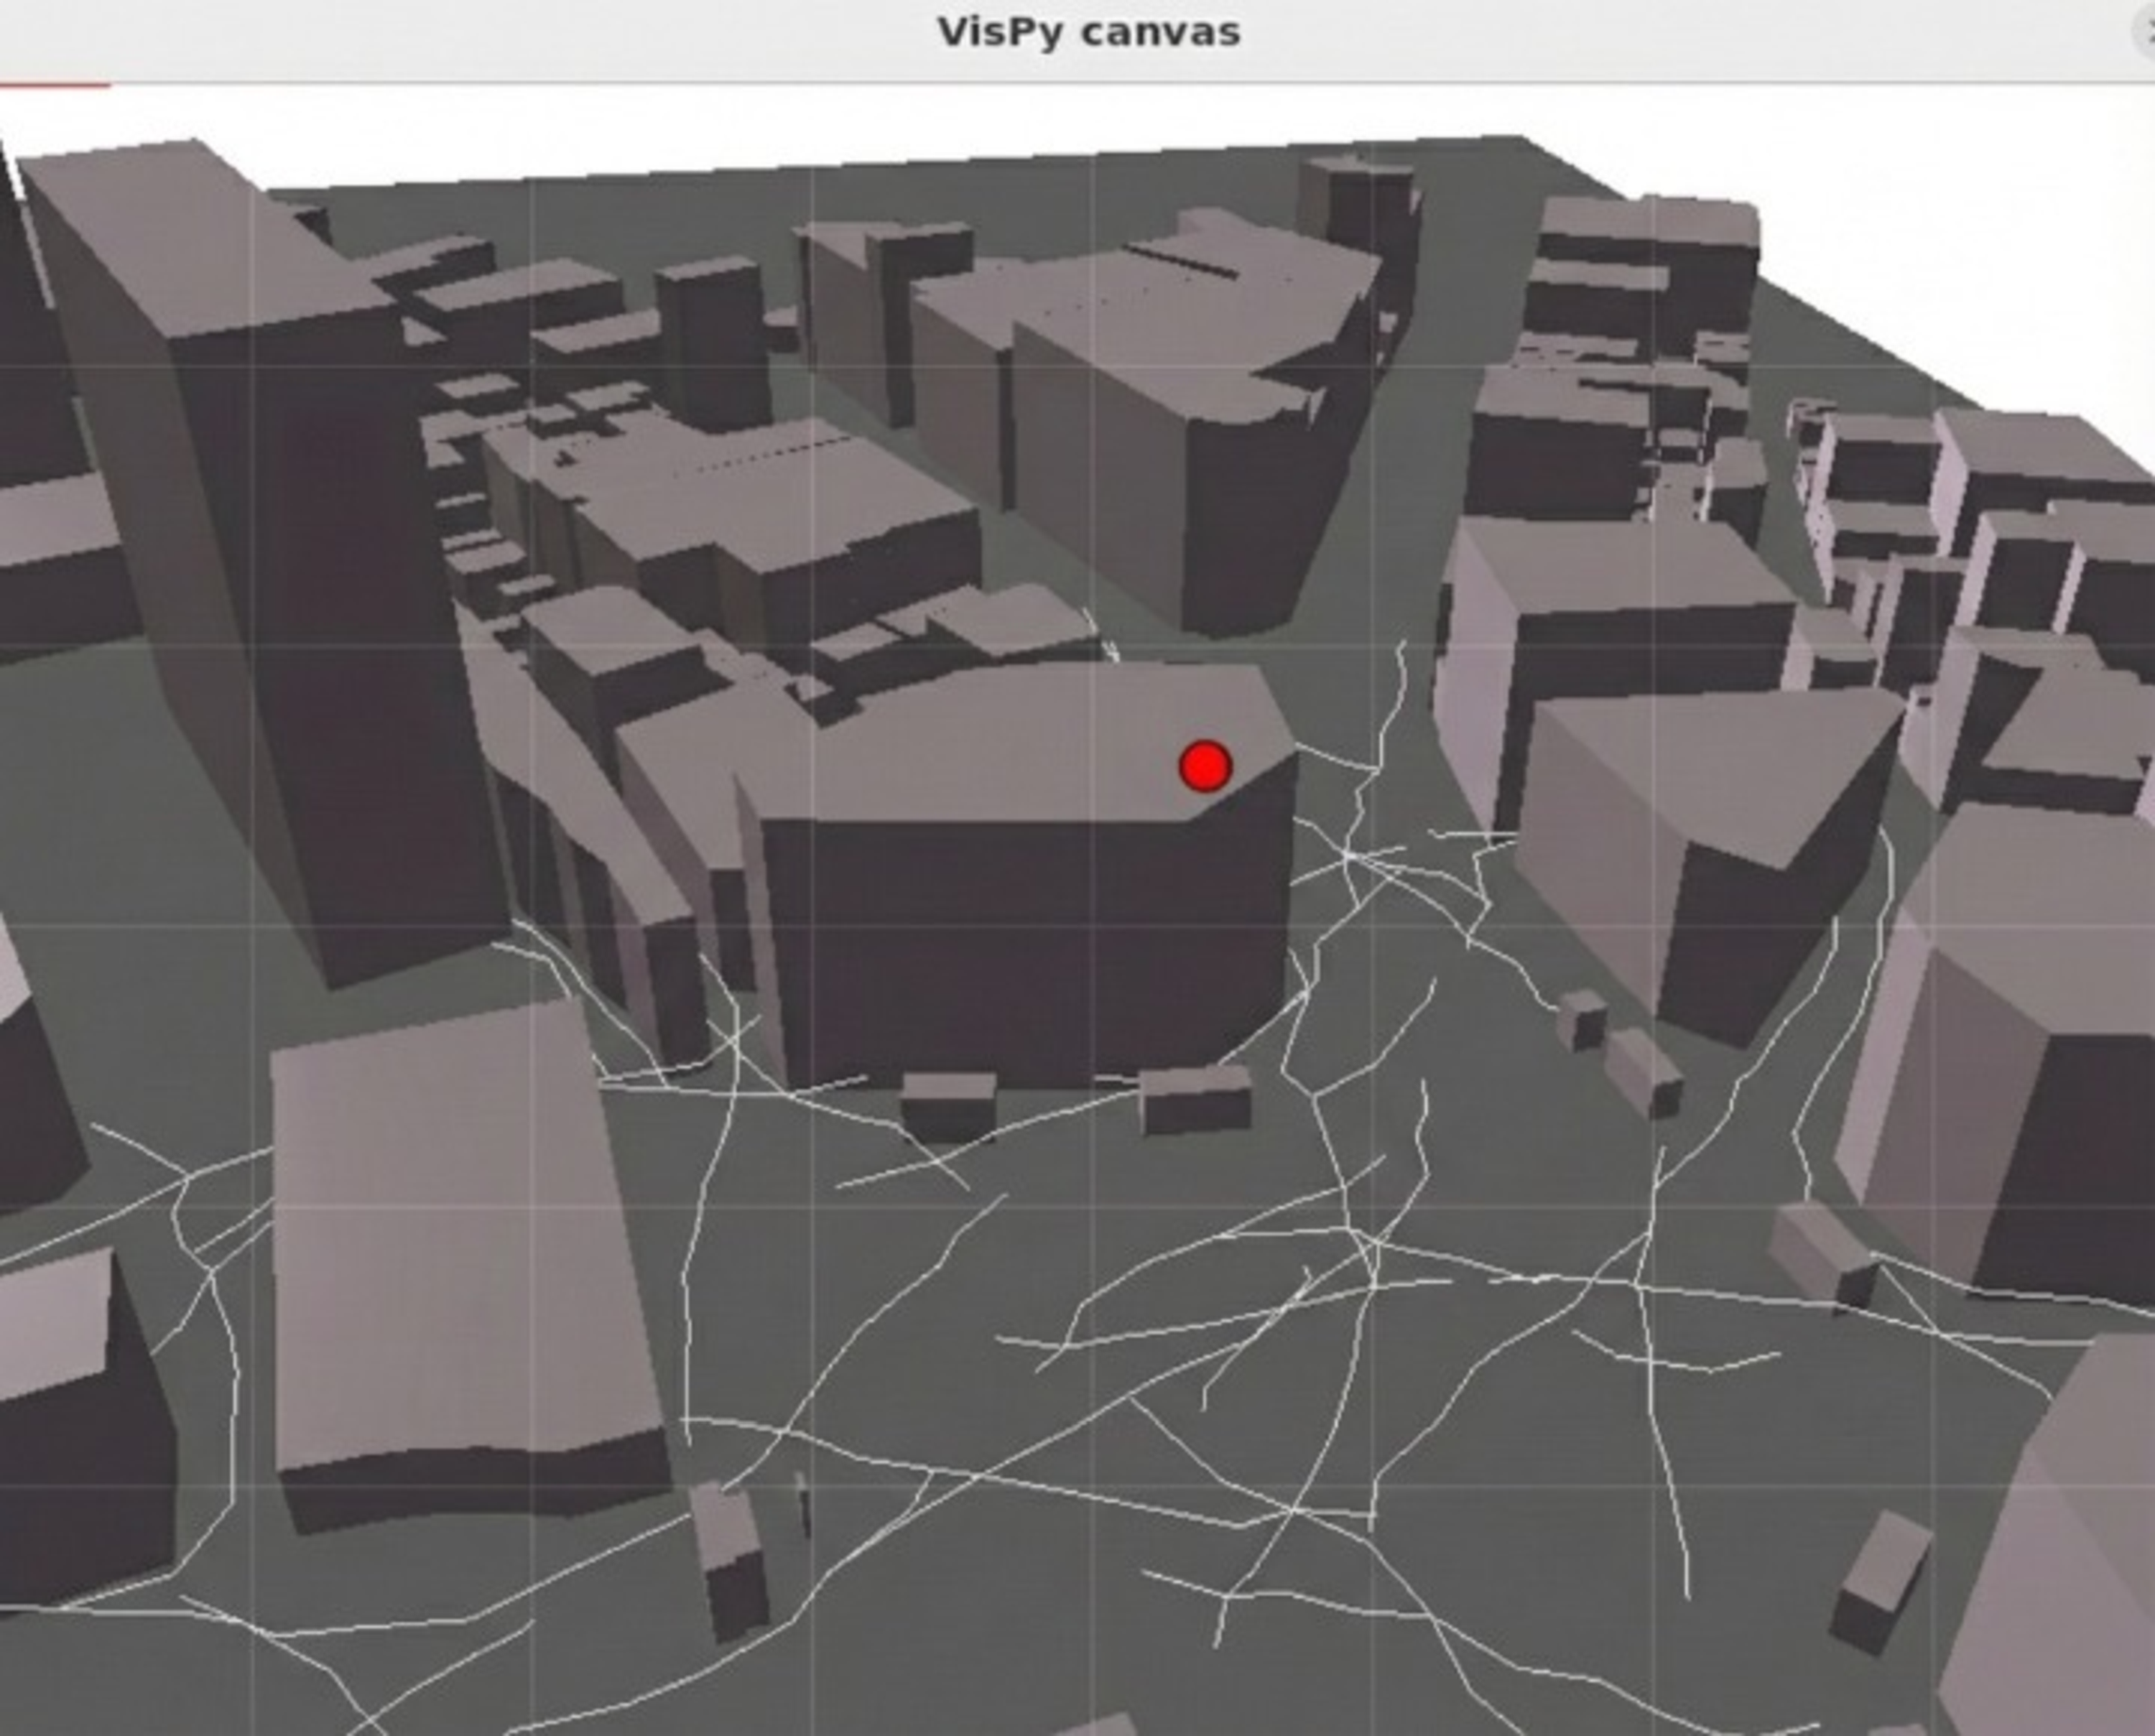
\includegraphics[width=\textwidth]{../picture/4nd/shibuya_2.png}
    \caption{渋谷(詳細2)}
    \label{fig:shibuya_2}
  \end{subfigure}

  \vspace{2mm}
  \begin{subfigure}{0.8\textwidth}
    \centering
    \includegraphics[width=\textwidth]{../picture/4nd/shibuya_fukan.png}
    \caption{渋谷(俯瞰)}
    \label{fig:shibuya_fukan}
  \end{subfigure}
  \caption{三次元モデル化に用いたエリア(渋谷)}
  \label{fig:area_shibuya}
\end{figure}

\begin{figure}[H]
  \centering
  \begin{subfigure}{0.49\textwidth}
    \centering
    \includegraphics[width=\textwidth]{../picture/4nd/shinjuku_1.png}
    \caption{新宿(詳細1)}
    \label{fig:shinjuku_1}
  \end{subfigure}
  \hfill
  \begin{subfigure}{0.49\textwidth}
    \centering
    \includegraphics[width=\textwidth]{../picture/4nd/shinjuku_2.png}
    \caption{新宿(詳細2)}
    \label{fig:shinjuku_2}
  \end{subfigure}
 
  \vspace{2mm}
  \begin{subfigure}{0.8\textwidth}
    \centering
    \includegraphics[width=\textwidth]{../picture/4nd/shinjuku_fukan.png}
    \caption{新宿(俯瞰)}
    \label{fig:shinjuku_fukan}
  \end{subfigure}
  \caption{三次元モデル化に用いたエリア(新宿)}
  \label{fig:area_shinjuku}
\end{figure}

\begin{figure}[H]
  \centering
  \begin{subfigure}{0.8\textwidth}
    \centering
    \includegraphics[width=\textwidth]{../picture/4nd/kinshityou.png}
    \caption{錦糸町(詳細)}
    \label{fig:kinshityou}
  \end{subfigure}

  \vspace{2mm}
  \begin{subfigure}{0.8\textwidth}
    \centering
    \includegraphics[width=\textwidth]{../picture/4nd/kinshityou_fukan.png}
    \caption{錦糸町(俯瞰)}
    \label{fig:kinshityou_fukan}
  \end{subfigure}
  \caption{三次元モデル化に用いたエリア(錦糸町)}
  \label{fig:area_kinshityou}
\end{figure}

\begin{figure}[H]
  \centering
  \begin{subfigure}{0.49\textwidth}
    \centering
    \includegraphics[width=\textwidth]{../picture/4nd/marunouchi_before_build.png}
    \caption{八重洲(ビル建設前)}
    \label{fig:marunouchi_before_build}
  \end{subfigure}
  \hfill
  \begin{subfigure}{0.49\textwidth}
    \centering
    \includegraphics[width=\textwidth]{../picture/4nd/marunouchi_built.png}
    \caption{八重洲(ビル建設後)}
    \label{fig:marunouchi_built}
  \end{subfigure}

  \vspace{2mm}
  \begin{subfigure}{0.8\textwidth}
    \centering
    \includegraphics[width=\textwidth]{../picture/4nd/marunouchi_fukan.png}
    \caption{八重洲(俯瞰)}
    \label{fig:marunouchi_fukan}
  \end{subfigure}
  \caption{三次元モデル化に用いたエリア(八重洲)}
  \label{fig:area_marunouchi}
\end{figure}









レイトレーシングの設定として用いたパラメータを示す.
建物には鉄の物性値を,地面には土の物性値を割り当てた.

\begin{align}
  \text{中心周波数:}\texttt{frequency} &= 3.5~\mathrm{GHz} \\
  \text{サブキャリア間隔:}\texttt{SCS} &= 15~\mathrm{kHz} \\
  \text{帯域幅:}\texttt{bandwidth} &= 20~\mathrm{MHz} \\
  \text{送信アンテナ数:}\texttt{numTx} &= 16 \\
  \text{受信アンテナ数:}\texttt{numRx} &= 2 \\
  \text{速度:}\texttt{velocity} &= 2~\mathrm{km/h},\,20~\mathrm{km/h} \\
  \text{サンプリング周波数:}\texttt{sampling\_frequency} &= 200~\mathrm{Hz} \\
  \text{最大反射回数:}\texttt{max\_reflections} &= 5 \\
  \text{基地局アンテナ縦方向素子間隔:}\texttt{base\_station\_antenna\_vertical\_spacing} &= 0.5 \\
  \text{基地局アンテナ横方向素子間隔:}\texttt{base\_station\_antenna\_horizontal\_spacing} &= 0.5 \\
  \text{端末アンテナ列数:}\texttt{user\_antenna\_rows} &= 2 \\
  \text{端末アンテナ行数:}\texttt{user\_antenna\_cols} &= 1 \\
  \text{端末アンテナ縦方向素子間隔:}\texttt{user\_antenna\_vertical\_spacing} &= 0.5 \\
  \text{端末アンテナ横方向素子間隔:}\texttt{user\_antenna\_horizontal\_spacing} &= 0.5 \\
  \text{反射:}\texttt{reflection} &= \texttt{true} \\
  \text{回折:}\texttt{diffraction} &= \texttt{true} \\
  \text{散乱:}\texttt{scattering} &= \texttt{false} \\
  \text{パス数上限:}\texttt{cir\_num\_paths} &= 200 \\
  \text{遅延の正規化:}\texttt{path.normalize\_delays} &= \texttt{true} \\
  \text{CIRからOFDMへの変換時の正規化:}\texttt{cir\_to\_ofdm\_normalize} &= \texttt{false}
\end{align}

上記の設定より,SRS送信間隔\texttt{srs\_sampling}は
\begin{equation}
  \texttt{srs\_sampling}=\frac{1}{\texttt{sampling\_frequency}}=\frac{1}{200~\mathrm{Hz}}=5~\mathrm{ms}
\end{equation}
となる.


SRSは周波数方向に一定間隔で配置されるとし,SRSが配置された周波数点においてCSIを算出する.
周波数方向のリソースブロック Resource Block, RBは,サブキャリア12本を束ねた単位であり,1RBの周波数幅は
\begin{equation}
  B_{\mathrm{RB}}=12\,SCS=12\times 15~\mathrm{kHz}=180~\mathrm{kHz}
\end{equation}
である.
本研究では,周波数方向に2RBおきにSRSを送信すると仮定する.すなわち,SRSが配置されるRBの間隔は
\begin{equation}
  B_{\mathrm{SRS}}=2\,B_{\mathrm{RB}}=360~\mathrm{kHz}
\end{equation}
である.このとき,CSIはSRSが配置されたRBで算出されるため,周波数方向のCSI系列は2RB間隔でサンプリングされたものとなる.

帯域端の影響を避けるため,本研究では帯域内の中心部分のみを用い,有効なRB数を\(N_{\mathrm{RB}}=96\)とする.
このとき,有効帯域幅は
\begin{equation}
  bandwidth_{\mathrm{eff}}=N_{\mathrm{RB}}\,B_{\mathrm{RB}}=96\times 180~\mathrm{kHz}=17.28~\mathrm{MHz}
\end{equation}
となる.2RBおきにSRSが配置されるため,CSIが算出されるRB数は
\begin{equation}
  N_{\mathrm{rb}}=\frac{N_{\mathrm{RB}}}{2}=\frac{96}{2}=48
\end{equation}
となる.以上より,帯域幅20~MHzでは1スロットあたり周波数方向に\(N_{\mathrm{rb}}=48\)個のRBでCSIが算出される.
以上の条件でレイトレーシングを実行し生成したCSI系列を[時間,リソースブロック,送信アンテナ,受信アンテナ,複素数次元]として保存する.



\subsection{シミュレーション条件}
\label{subsec:simulation_conditions}

本節では,補間手法評価のためのシミュレーション方法について述べる.
補間精度の評価には,第\ref{subsec:terrain_raytracing}節で述べた錦糸町および丸の内の2種類の地形データに対してレイトレーシングにより生成したCSI系列を用いる.
補間手法としては,第\ref{sec:interpolation_methods}節で述べた線形補間,スプライン補間,低次多項式近似,ニューラルネットワーク補間を比較対象とする.
ニューラルネットワーク補間器の学習には,評価対象とは異なる地形データから生成したCSI系列を用いる.
錦糸町駅前のCSI系列を補間するモデルは,新宿,池袋,渋谷の3地点から生成したCSI系列で学習する.
丸の内駅前のCSI系列を補間するモデルは,丸の内駅前から生成したCSI系列を学習データとして用いる.
前者は他セルで運用していた補間器を新規基地局へ展開する状況を想定しており,後者は同一セル内で環境変動が生じた際に補間器を再学習する状況を想定している.

補間器の構成は第\ref{sec:interpolation_methods}節で述べたMLPであり,$\mathrm{Linear}(6F\rightarrow 2048)\rightarrow \mathrm{ReLU}\rightarrow\mathrm{Linear}(2048\rightarrow 1024)\rightarrow \mathrm{ReLU}\rightarrow\mathrm{Linear}(1024\rightarrow F)$の3層構造とする.
学習時の損失関数には補間値$\widetilde{\bm{H}}_t$と真値$\bm{H}_t$の平均二乗誤差を用い,最適化にはAdamを使用する.
学習率は$10^{-4}$,バッチサイズは128,エポック数は10とする.

パイロット信号の送信周期が変化した場合における補間精度を評価するため,推定値と予測対象の割合を変化させた複数の観測パターンを設定する.
観測パターンは,周期$P$の文字列として$\mathrm{S}$を観測時刻,$\mathrm{P}$を欠損時刻として定義し,以下の3種類を用いる.
\begin{align}
\text{SSSP} &: \; \mathrm{S},\mathrm{S},\mathrm{S},\mathrm{P} \; \text{を周期 }P=4\text{で繰り返し} \\
\text{SSP}  &: \; \mathrm{S},\mathrm{S},\mathrm{P} \; \text{を周期 }P=3\text{で繰り返し} \\
\text{SP}   &: \; \mathrm{S},\mathrm{P} \; \text{を周期 }P=2\text{で繰り返し}
\end{align}
SSSPでは4スロットに1回,SSPでは3スロットに1回,SPでは2スロットに1回の頻度で欠損が発生する.
観測パターンに応じて欠損率が25\%から50\%まで変化するため,各パターンにおいて有効な補間手法を特定する.
補間対象となる時刻集合$\mathcal{T}_P$は$\mathcal{T}_P \triangleq \{t \mid t \bmod P = P-1\}$として定義し,観測時刻集合は$\mathcal{T}_S=\{0,1,\dots,T-1\}\setminus\mathcal{T}_P$とする.

評価指標には正規化平均二乗誤差NMSEを用いる.
補間対象時刻$t\in\mathcal{T}_P$における補間値$\widetilde{\bm{H}}_t$と真値$\bm{H}_t$の誤差を
\begin{equation}
  \mathrm{NMSE}(t)
  =\frac{\left\lVert \widetilde{\bm{H}}_t-\bm{H}_t\right\rVert_2^2}{\left\lVert \bm{H}_t\right\rVert_2^2}
  \label{eq:nmse_interp}
\end{equation}
として定義する.
全ファイルおよび全補間対象時刻に対してNMSEを算出し,その平均値
\begin{equation}
\overline{\mathrm{NMSE}}
=
\frac{1}{N}\sum_{n=1}^{N}\mathrm{NMSE}(t_n)
\end{equation}
を最終的な評価スコアとする.ここで$N$は評価に用いた補間対象時刻の総数である.



\section{地形ごとの補間手法比較評価}

\subsection{結果}
本節では,各地形データから生成したCSI系列に対する補間精度の評価結果を示す.
評価はSSSPパターンを用いて実施し,各補間手法のNMSEを比較する.

\subsubsection{錦糸町データセットにおける補間精度}
錦糸町駅前の地形データから生成した284ファイルのCSI系列に対する補間精度評価を表\ref{tab:kinshicho_sssp_results}に示す.
多項式近似の設定において,次数と片側近傍点数を記載する.例えば「4次,片側3点ずつ」は4次多項式を用い,補間対象時刻の前後それぞれ3点ずつ,計6点の推定値を近傍として使用することを意味する.
ニューラルネットワーク補間の設定において,$c$はコンテキストサイズを表す.

\begin{table}[H]
  \centering
  \caption{錦糸町データセットにおけるSSSPパターンの補間精度}
  \label{tab:kinshicho_sssp_results}
  \begin{tabular}{llc}
    \hline
    手法 & 設定 & NMSE \\
    \hline
    線形補間 & -- & 0.3748 \\
    スプライン補間 & -- & \textbf{0.0061} \\
    多項式近似 & 2次,片側3点ずつ & 0.0517 \\
    多項式近似 & 3次,片側3点ずつ & 0.0517 \\
    多項式近似 & 4次,片側3点ずつ & \textbf{0.0059} \\
    多項式近似 & 5次,片側3点ずつ & \textbf{0.0059} \\
    多項式近似 & 6次,片側3点ずつ & 0.1432 \\
    多項式近似 & 4次,片側6点ずつ & 0.2288 \\
    多項式近似 & 4次,片側9点ずつ & 0.2584 \\
    ニューラルネットワーク補間 & $c=1$ & 0.3853 \\
    ニューラルネットワーク補間 & $c=2$ & 0.5112 \\
    ニューラルネットワーク補間 & $c=3$ & 0.4737 \\
    \hline
  \end{tabular}
\end{table}

スプライン補間および4次または5次の多項式近似がNMSE 0.006程度で最良の精度を達成した.
一方,線形補間やニューラルネットワーク補間はNMSE 0.37以上と低い精度にとどまった.
ニューラルネットワークが低精度となった要因として,学習データが錦糸町と異なる3地点で構成されているため,チャネル特性の違いに対応できなかったことが考えられる.





\subsubsection{丸の内(LoS)データセットにおける補間精度}
丸の内(LoS)の地形データから生成した101ファイルのCSI系列に対する補間精度評価を表\ref{tab:marunouchi_sssp_results}に示す.

\begin{table}[H]
  \centering
  \caption{丸の内(LoS)データセットにおけるSSSPパターンの補間精度}
  \label{tab:marunouchi_sssp_results}
  \begin{tabular}{llc}
    \hline
    手法 & 設定 & NMSE \\
    \hline
    線形補間 & -- & 0.1644 \\
    スプライン補間 & -- & \textbf{0.0456} \\
    多項式近似 & 2次,片側3点ずつ & 0.0576 \\
    多項式近似 & 3次,片側3点ずつ & 0.0576 \\
    多項式近似 & 4次,片側3点ずつ & \textbf{0.0463} \\
    多項式近似 & 5次,片側3点ずつ & \textbf{0.0463} \\
    多項式近似 & 6次,片側3点ずつ & 0.1517 \\
    多項式近似 & 4次,片側6点ずつ & 0.1517 \\
    多項式近似 & 4次,片側9点ずつ & 0.1571 \\
    ニューラルネットワーク補間 & $c=1$ & 0.1453 \\
    ニューラルネットワーク補間 & $c=2$ & 0.1314 \\
    ニューラルネットワーク補間 & $c=3$ & 0.4911 \\
    \hline
  \end{tabular}
\end{table}

丸の内(NLoS)データセットに対するSSSPパターンの補間精度評価を表\ref{tab:marunouchi_nlos_sssp_results}に示す.
丸の内(NLoS)データセットの評価では,線形補間およびニューラルネットワーク補間を比較対象から除外した.
錦糸町および丸の内(LoS)データセットの評価において,線形補間は補間対象の前後1点のみを用いる単純な手法であり,NMSEが0.16から0.37と低精度であることが確認された.
ニューラルネットワーク補間も学習データと評価データの地点差に起因するドメインシフトにより解析的手法を下回る精度にとどまった.
これらの結果から,丸の内(NLoS)データセットにおいても同様の傾向が予想されるため,評価対象から除外した.

\begin{table}[H]
  \centering
  \caption{丸の内(NLoS)データセットにおけるSSSPパターンの補間精度}
  \label{tab:marunouchi_nlos_sssp_results}
  \begin{tabular}{llc}
    \hline
    手法 & 設定 & NMSE \\
    \hline
    スプライン補間 & -- & \textbf{0.057395} \\
    多項式近似 & 2次,片側3点ずつ & 0.082413 \\
    多項式近似 & 3次,片側3点ずつ & 0.082413 \\
    多項式近似 & 4次,片側3点ずつ & 0.057968 \\
    多項式近似 & 5次,片側3点ずつ & 0.057968 \\
    多項式近似 & 6次,片側3点ずつ & 0.173984 \\
    多項式近似 & 4次,片側6点ずつ & 0.213839 \\
    多項式近似 & 4次,片側9点ずつ & 0.224907 \\
    \hline
  \end{tabular}
\end{table}

丸の内(LoS)データセットにおいても,スプライン補間と4次または5次の多項式近似が最良の精度を示し,NMSEは0.04から0.05程度であった.
ニューラルネットワーク補間の精度は錦糸町データセットと比較して向上している.これは,丸の内(LoS)データセットでは学習と評価が同一地点のCSI系列で構成されているためである.
両データセットを通じて,スプライン補間と4次多項式近似が一貫して高い補間精度を達成した.
多項式近似では,次数4と次数5で同一のNMSEを示した.これは総近傍点数$K=6$($k=3$)に対して次数5の多項式が過剰適合となり,事実上4次と同等の近似となったためと考えられる.
次数6では精度が大幅に低下しており,過学習による悪影響が確認された.
近傍点数を増やした場合においても精度が低下しており,補間対象から離れた時刻の推定値は精度向上に寄与しないことが示された.


\section{パイロット疎化拡大時の補間精度評価}
本節では,パイロット信号の送信頻度をさらに低減した場合の補間精度を評価する.
前節ではSSSPパターンを用いて評価したが,本節ではSSPパターンおよびSPパターンを追加し,欠損率が33\%および50\%に増加した場合の補間精度を比較する.

\subsection{結果}

\subsubsection{錦糸町データセットにおける補間精度}
錦糸町データセットに対するSSPパターンおよびSPパターンの補間精度評価を表\ref{tab:kinshicho_ssp_sp_results}に示す.

\begin{table}[H]
  \centering
  \caption{錦糸町データセットにおけるSSPおよびSPパターンの補間精度}
  \label{tab:kinshicho_ssp_sp_results}
  \begin{tabular}{llrr}
    \hline
    手法 & 設定 & SSP & SP \\
    \hline
    線形補間 & -- & 0.2751 & 0.2865 \\
    スプライン補間 & -- & \textbf{0.0062} & \textbf{0.0130} \\
    多項式近似 & 2次,片側3点ずつ & 0.1174 & 0.1757 \\
    多項式近似 & 3次,片側3点ずつ & 0.1174 & 0.1757 \\
    多項式近似 & 4次,片側3点ずつ & \textbf{0.0069} & \textbf{0.0162} \\
    多項式近似 & 5次,片側3点ずつ & \textbf{0.0069} & \textbf{0.0162} \\
    多項式近似 & 6次,片側3点ずつ & 0.1588 & 0.2184 \\
    多項式近似 & 4次,片側6点ずつ & 0.1627 & 0.2242 \\
    多項式近似 & 4次,片側9点ずつ & 0.2795 & 0.3130 \\
    ニューラルネットワーク補間 & $c=1$ & 0.3121 & 0.3781 \\
    ニューラルネットワーク補間 & $c=2$ & 0.4268 & 0.3968 \\
    ニューラルネットワーク補間 & $c=3$ & 0.5761 & 0.5961 \\
    \hline
  \end{tabular}
\end{table}

SSPパターンにおいても,スプライン補間と4次多項式近似が最良の精度を示し,NMSEは0.006から0.007程度であった.
SPパターンでは欠損率が50\%に達するが,スプライン補間と4次多項式近似はNMSE 0.013から0.016程度を維持した.
ニューラルネットワーク補間は全パターンで0.3以上のNMSEとなり,学習データと評価データの地点差による汎化性能の低さが確認された.

以降のSPP/SPPPパターンの評価では,線形補間およびニューラルネットワーク補間を比較対象から除外した.
SSSP/SSP/SPパターンの評価において,線形補間はNMSEが0.16から0.37と低精度であり,補間対象の前後1点のみを用いる単純な手法では時間変動を十分に捉えられないことが確認された.
ニューラルネットワーク補間も同様に精度が低く,学習データと評価データの地点差に起因するドメインシフトにより,スプライン補間や多項式近似といった解析的手法を下回る結果となった.
連続補間パターンでは単一フレーム補間よりも推定が困難であり,これらの手法の精度低下が予想されるため,評価対象から除外した.

\noindent
錦糸町データセットに対するSPPパターン(周期3,2フレーム連続補間)およびSPPPパターン(周期4,3フレーム連続補間)の補間精度評価をそれぞれ表\ref{tab:kinshicho_spp_results}および表\ref{tab:kinshicho_sppp_results}に示す.
本実験では補間位置が複数存在するため,補間位置ごとのNMSE(pos)と,それらを統合したOverall NMSEを算出した.

\begin{table}[H]
  \centering
  \caption{錦糸町データセットにおけるSPPパターン(周期3,2フレーム連続補間)の補間精度}
  \label{tab:kinshicho_spp_results}
  \begin{tabular}{llrrr}
    \hline
    手法 & 設定 & Overall NMSE & pos0 & pos1 \\
    \hline
    多項式近似 & 5次,片側3点ずつ & \textbf{0.1286} & 0.1283 & 0.1288 \\
    スプライン補間 & 片側3点ずつ & 0.1314 & 0.1311 & 0.1317 \\
    スプライン補間 & 片側6点ずつ & 0.1364 & 0.1361 & 0.1366 \\
    スプライン補間 & 片側9点ずつ & 0.1364 & 0.1361 & 0.1367 \\
    多項式近似 & 4次,片側3点ずつ & 0.1691 & 0.1690 & 0.1691 \\
    多項式近似 & 3次,片側3点ずつ & 0.2453 & 0.2456 & 0.2449 \\
    多項式近似 & 2次,片側3点ずつ & 0.2491 & 0.2497 & 0.2485 \\
    多項式近似 & 6次,片側6点ずつ & 0.2650 & 0.2654 & 0.2646 \\
    多項式近似 & 5次,片側6点ずつ & 0.3092 & 0.3096 & 0.3088 \\
    多項式近似 & 4次,片側6点ずつ & 0.3116 & 0.3122 & 0.3110 \\
    多項式近似 & 6次,片側9点ずつ & 0.3366 & 0.3372 & 0.3360 \\
    多項式近似 & 5次,片側9点ずつ & 0.3709 & 0.3714 & 0.3705 \\
    多項式近似 & 4次,片側9点ずつ & 0.3711 & 0.3718 & 0.3703 \\
    多項式近似 & 6次,片側3点ずつ & 0.4187 & 0.4188 & 0.4186 \\
    \hline
  \end{tabular}
\end{table}

\begin{table}[H]
  \centering
  \caption{錦糸町データセットにおけるSPPPパターン(周期4,3フレーム連続補間)の補間精度}
  \label{tab:kinshicho_sppp_results}
  \begin{tabular}{llrrrr}
    \hline
    手法 & 設定 & Overall NMSE & pos0 & pos1 & pos2 \\
    \hline
    多項式近似 & 5次,片側3点ずつ & \textbf{0.2756} & 0.2088 & 0.4091 & 0.2088 \\
    スプライン補間 & 片側3点ずつ & 0.2822 & 0.2128 & 0.4209 & 0.2129 \\
    スプライン補間 & 片側6点ずつ & 0.2830 & 0.2134 & 0.4219 & 0.2136 \\
    スプライン補間 & 片側9点ずつ & 0.2830 & 0.2134 & 0.4218 & 0.2136 \\
    多項式近似 & 4次,片側3点ずつ & 0.3359 & 0.2992 & 0.4091 & 0.2993 \\
    多項式近似 & 3次,片側3点ずつ & 0.3454 & 0.3236 & 0.3895 & 0.3230 \\
    多項式近似 & 6次,片側6点ずつ & 0.3518 & 0.3381 & 0.3800 & 0.3372 \\
    多項式近似 & 2次,片側3点ずつ & 0.3652 & 0.3537 & 0.3895 & 0.3525 \\
    多項式近似 & 5次,片側6点ずつ & 0.3652 & 0.3599 & 0.3755 & 0.3604 \\
    多項式近似 & 4次,片側6点ずつ & 0.3708 & 0.3687 & 0.3755 & 0.3683 \\
    多項式近似 & 6次,片側9点ずつ & 0.3787 & 0.3769 & 0.3828 & 0.3764 \\
    多項式近似 & 5次,片側9点ずつ & 0.4033 & 0.4016 & 0.4054 & 0.4028 \\
    多項式近似 & 4次,片側9点ずつ & 0.4041 & 0.4035 & 0.4054 & 0.4035 \\
    多項式近似 & 6次,片側3点ずつ & 0.5047 & 0.3987 & 0.7272 & 0.3880 \\
    \hline
  \end{tabular}
\end{table}





\subsubsection{丸の内(LoS)データセットにおける補間精度}
丸の内(LoS)データセットに対するSSPパターンおよびSPパターンの補間精度評価を表\ref{tab:marunouchi_ssp_sp_results}に示す.

\begin{table}[H]
  \centering
  \caption{丸の内(LoS)データセットにおけるSSPおよびSPパターンの補間精度}
  \label{tab:marunouchi_ssp_sp_results}
  \begin{tabular}{llrr}
    \hline
    手法 & 設定 & SSP & SP \\
    \hline
    線形補間 & -- & 0.1380 & 0.1474 \\
    スプライン補間 & -- & \textbf{0.0278} & \textbf{0.0360} \\
    多項式近似 & 2次,片側3点ずつ & 0.0969 & 0.1177 \\
    多項式近似 & 3次,片側3点ずつ & 0.0969 & 0.1177 \\
    多項式近似 & 4次,片側3点ずつ & \textbf{0.0278} & \textbf{0.0370} \\
    多項式近似 & 5次,片側3点ずつ & \textbf{0.0278} & \textbf{0.0370} \\
    多項式近似 & 6次,片側3点ずつ & 0.1638 & 0.2244 \\
    多項式近似 & 4次,片側6点ずつ & 0.1070 & 0.1324 \\
    多項式近似 & 4次,片側9点ずつ & 0.1326 & 0.1431 \\
    ニューラルネットワーク補間 & $c=1$ & 0.1401 & 0.1424 \\
    ニューラルネットワーク補間 & $c=2$ & 0.1967 & 0.1658 \\
    ニューラルネットワーク補間 & $c=3$ & 0.1743 & 0.2269 \\
    \hline
  \end{tabular}
\end{table}





\noindent
丸の内(LoS)データセットに対するSPPパターン(周期3,2フレーム連続補間)およびSPPPパターン(周期4,3フレーム連続補間)の補間精度評価をそれぞれ表\ref{tab:marunouchi_los_spp_results}および表\ref{tab:marunouchi_los_sppp_results}に示す.
本実験では補間位置が複数存在するため,補間位置ごとのNMSE(pos)と,それらを統合したOverall NMSEを算出した.

\begin{table}[H]
  \centering
  \caption{丸の内(LoS)データセットにおけるSPPパターン(周期3,2フレーム連続補間)の補間精度}
  \label{tab:marunouchi_los_spp_results}
  \begin{tabular}{llrrr}
    \hline
    手法 & 設定 & Overall NMSE & pos0 & pos1 \\
    \hline
    多項式近似 & 5次,片側3点ずつ & \textbf{0.1675} & 0.1645 & 0.1706 \\
    スプライン補間 & 片側3点ずつ & 0.1742 & 0.1712 & 0.1773 \\
    スプライン補間 & 片側6点ずつ & 0.1756 & 0.1756 & 0.1756 \\
    スプライン補間 & 片側9点ずつ & 0.1757 & 0.1757 & 0.1757 \\
    多項式近似 & 3次,片側3点ずつ & 0.1793 & 0.1792 & 0.1794 \\
    多項式近似 & 6次,片側6点ずつ & 0.1827 & 0.1826 & 0.1829 \\
    多項式近似 & 2次,片側3点ずつ & 0.1845 & 0.1807 & 0.1884 \\
    多項式近似 & 4次,片側3点ずつ & 0.1992 & 0.1908 & 0.2076 \\
    多項式近似 & 5次,片側6点ずつ & 0.2251 & 0.2252 & 0.2250 \\
    多項式近似 & 4次,片側6点ずつ & 0.2260 & 0.2258 & 0.2262 \\
    多項式近似 & 6次,片側9点ずつ & 0.2262 & 0.2261 & 0.2263 \\
    多項式近似 & 4次,片側9点ずつ & 0.2566 & 0.2565 & 0.2567 \\
    多項式近似 & 5次,片側9点ずつ & 0.2566 & 0.2567 & 0.2566 \\
    多項式近似 & 6次,片側3点ずつ & 0.4523 & 0.4524 & 0.4521 \\
    \hline
  \end{tabular}
\end{table}

\begin{table}[H]
  \centering
  \caption{丸の内(LoS)データセットにおけるSPPPパターン(周期4,3フレーム連続補間)の補間精度}
  \label{tab:marunouchi_los_sppp_results}
  \begin{tabular}{llrrrr}
    \hline
    手法 & 設定 & Overall NMSE & pos0 & pos1 & pos2 \\
    \hline
    多項式近似 & 5次,片側3点ずつ & \textbf{0.2565} & 0.2039 & 0.3600 & 0.2057 \\
    スプライン補間 & 片側6点ずつ & 0.2615 & 0.2088 & 0.3696 & 0.2061 \\
    スプライン補間 & 片側9点ずつ & 0.2617 & 0.2090 & 0.3698 & 0.2062 \\
    スプライン補間 & 片側3点ずつ & 0.2618 & 0.2079 & 0.3682 & 0.2092 \\
    多項式近似 & 3次,片側3点ずつ & 0.2717 & 0.2441 & 0.3236 & 0.2474 \\
    多項式近似 & 5次,片側6点ずつ & 0.2761 & 0.2614 & 0.3068 & 0.2601 \\
    多項式近似 & 4次,片側6点ずつ & 0.2813 & 0.2687 & 0.3068 & 0.2684 \\
    多項式近似 & 6次,片側9点ずつ & 0.2868 & 0.2754 & 0.3097 & 0.2753 \\
    多項式近似 & 2次,片側3点ずつ & 0.2871 & 0.2645 & 0.3236 & 0.2732 \\
    多項式近似 & 6次,片側6点ずつ & 0.2879 & 0.2645 & 0.3353 & 0.2641 \\
    多項式近似 & 4次,片側3点ずつ & 0.2907 & 0.2470 & 0.3600 & 0.2649 \\
    多項式近似 & 5次,片側9点ずつ & 0.2945 & 0.2893 & 0.3060 & 0.2883 \\
    多項式近似 & 4次,片側9点ずつ & 0.2975 & 0.2933 & 0.3060 & 0.2933 \\
    多項式近似 & 6次,片側3点ずつ & 0.5428 & 0.4325 & 0.7700 & 0.4260 \\
    \hline
  \end{tabular}
\end{table}

丸の内(LoS)データセットにおいても同様の傾向が確認された.
スプライン補間と4次多項式近似はSSPパターンでNMSE 0.03程度,SPパターンでNMSE 0.04程度を達成した.
ニューラルネットワーク補間は錦糸町データセットと比較して精度が向上しており,同一地点での学習による効果が認められる.
ただし,スプライン補間や4次多項式近似には及ばず,学習ベースの補間器が解析的手法を上回る条件は本評価では見出されなかった.







丸の内(NLoS)データセットに対するSSPパターンおよびSPパターンの補間精度評価を表\ref{tab:marunouchi_nlos_ssp_sp_results}に示す.

\begin{table}[H]
  \centering
  \caption{丸の内(NLoS)データセットにおけるSSPおよびSPパターンの補間精度}
  \label{tab:marunouchi_nlos_ssp_sp_results}
  \begin{tabular}{llrr}
    \hline
    手法 & 設定 & SSP & SP \\
    \hline
    スプライン補間 & 片側3点ずつ & 0.054962 & \textbf{0.053230} \\
    多項式近似 & 2次,片側3点ずつ & 0.134070 & 0.170361 \\
    多項式近似 & 3次,片側3点ずつ & 0.134070 & 0.170361 \\
    多項式近似 & 4次,片側3点ずつ & \textbf{0.054486} & 0.054971 \\
    多項式近似 & 5次,片側3点ずつ & \textbf{0.054486} & 0.054971 \\
    多項式近似 & 6次,片側3点ずつ & 0.189349 & 0.249500 \\
    多項式近似 & 4次,片側6点ずつ & 0.159744 & 0.193791 \\
    多項式近似 & 4次,片側9点ずつ & 0.217653 & 0.280060 \\
    \hline
  \end{tabular}
\end{table}

\noindent
丸の内(NLoS)データセットに対するSPPパターン(周期3,2フレーム連続補間)およびSPPPパターン(周期4,3フレーム連続補間)の補間精度評価をそれぞれ表\ref{tab:marunouchi_nlos_spp_results}および表\ref{tab:marunouchi_nlos_sppp_results}に示す.
本実験では補間位置が複数存在するため,補間位置ごとのNMSE(pos)と,それらを統合したOverall NMSEを算出した.

\begin{table}[H]
  \centering
  \caption{丸の内(NLoS)データセットにおけるSPPパターン(周期3,2フレーム連続補間)の補間精度}
  \label{tab:marunouchi_nlos_spp_results}
  \begin{tabular}{llrrr}
    \hline
    手法 & 設定 & Overall NMSE & pos0 & pos1 \\
    \hline
    多項式近似 & 2次,片側3点ずつ & 0.212486 & 0.212546 & 0.212427 \\
    多項式近似 & 3次,片側3点ずつ & 0.208927 & 0.208889 & 0.208965 \\
    多項式近似 & 4次,片側3点ずつ & 0.182280 & 0.182264 & 0.182297 \\
    多項式近似 & 5次,片側3点ずつ & \textbf{0.152921} & 0.152825 & 0.153017 \\
    多項式近似 & 6次,片側3点ずつ & 0.458041 & 0.458171 & 0.457911 \\
    多項式近似 & 4次,片側6点ずつ & 0.281313 & 0.281317 & 0.281308 \\
    多項式近似 & 5次,片側6点ずつ & 0.278874 & 0.278817 & 0.278931 \\
    多項式近似 & 6次,片側6点ずつ & 0.210491 & 0.210727 & 0.210256 \\
    多項式近似 & 4次,片側9点ずつ & 0.345813 & 0.345677 & 0.345950 \\
    多項式近似 & 5次,片側9点ずつ & 0.345791 & 0.345676 & 0.345906 \\
    多項式近似 & 6次,片側9点ずつ & 0.308767 & 0.308690 & 0.308845 \\
    スプライン補間 & 片側3点ずつ & 0.157235 & 0.157129 & 0.157342 \\
    スプライン補間 & 片側6点ずつ & 0.160927 & 0.160826 & 0.161027 \\
    スプライン補間 & 片側9点ずつ & 0.160998 & 0.160898 & 0.161098 \\
    \hline
  \end{tabular}
\end{table}

\begin{table}[H]
  \centering
  \caption{丸の内(NLoS)データセットにおけるSPPPパターン(周期4,3フレーム連続補間)の補間精度}
  \label{tab:marunouchi_nlos_sppp_results}
  \begin{tabular}{llrrrr}
    \hline
    手法 & 設定 & Overall NMSE & pos0 & pos1 & pos2 \\
    \hline
    多項式近似 & 2次,片側3点ずつ & 0.317059 & 0.305640 & 0.339997 & 0.305541 \\
    多項式近似 & 3次,片側3点ずつ & 0.298134 & 0.277190 & 0.339997 & 0.277216 \\
    多項式近似 & 4次,片側3点ずつ & 0.300981 & 0.267654 & 0.368069 & 0.267219 \\
    多項式近似 & 5次,片側3点ずつ & \textbf{0.261897} & 0.209025 & 0.368069 & 0.208598 \\
    多項式近似 & 6次,片側3点ずつ & 0.548121 & 0.437063 & 0.780505 & 0.426793 \\
    多項式近似 & 4次,片側6点ずつ & 0.361749 & 0.353657 & 0.377893 & 0.353699 \\
    多項式近似 & 5次,片側6点ずつ & 0.357749 & 0.347582 & 0.377893 & 0.347772 \\
    多項式近似 & 6次,片側6点ずつ & 0.324681 & 0.309704 & 0.354742 & 0.309596 \\
    多項式近似 & 4次,片側9点ずつ & 0.376005 & 0.373168 & 0.381733 & 0.373114 \\
    多項式近似 & 5次,片側9点ずつ & 0.374111 & 0.370286 & 0.381733 & 0.370314 \\
    多項式近似 & 6次,片側9点ずつ & 0.361447 & 0.354386 & 0.375723 & 0.354233 \\
    スプライン補間 & 片側3点ずつ & 0.268611 & 0.213832 & 0.378606 & 0.213396 \\
    スプライン補間 & 片側6点ずつ & 0.270807 & 0.215560 & 0.381694 & 0.215167 \\
    スプライン補間 & 片側9点ずつ & 0.270968 & 0.215650 & 0.381976 & 0.215277 \\
    \hline
  \end{tabular}
\end{table}

SSSP/SSP/SPパターンを通じた結果を総括する.
表\ref{tab:summary_all_patterns}に,SSSP/SSP/SPパターンにおける各手法の平均NMSEを示す.

\begin{table}[H]
  \centering
  \caption{SSSP/SSP/SPパターンにおける平均NMSE}
  \label{tab:summary_all_patterns}
  \begin{tabular}{llrrr}
    \hline
    手法 & 設定 & 錦糸町 & 丸の内(LoS) & 丸の内(NLoS) \\
    \hline
    スプライン補間 & -- & 0.0084 & 0.0365 & 0.0552 \\
    多項式近似 & 4次,片側3点ずつ & 0.0097 & 0.0370 & 0.0558 \\
    多項式近似 & 5次,片側3点ずつ & 0.0097 & 0.0370 & 0.0558 \\
    \hline
  \end{tabular}
\end{table}

スプライン補間と4次多項式近似は,パイロット疎化率が25\%から50\%に変化しても安定した補間精度を維持した.
錦糸町では両手法の平均NMSEは0.01以下であり,丸の内(LoS)では0.04以下,丸の内(NLoS)においても0.06未満を維持した.
本評価の結果から,チャネル予測モデルの重み更新に用いる補間手法として,スプライン補間または4次多項式近似が有効であることが示唆された.


\section{おわりに}
本章では,チャネル予測モデルの重み更新に用いる補間手法を選定するため,錦糸町駅前と丸の内駅前の2種類の地形データから生成したCSI系列に対して補間精度の比較実験を実施した.
比較対象として,スプライン補間および多項式近似を用いた.

実験の結果,スプライン補間と4次多項式近似が両データセットで最良の精度を達成し,錦糸町ではNMSEは0.01以下,丸の内では0.04から0.06程度であった.
パイロット信号の送信頻度を低減し欠損率が25\%から50\%に増加した場合においても,両手法は安定した補間精度を維持した.

以上の結果から,次章以降の実験ではスプライン補間または4次多項式近似を用いて提案機構を実装する.


% 電磁界シミュレーション評価
\chapter{時系列補間型学習データを用いた無線チャネル予測機構}{}
\label{chap:4th}

\section{はじめに}
本章では,第2章で指摘した予測スロットにおいて推定値が得られずモデルの重みを更新できないという問題に対して
補間を用いた新たなモデル重み更新機構を提案する.その際に用いる補間手法は第3章で比較検証した中で最も有効な手法を採用する.



\section{時系列補間型学習データを用いたチャネル予測機構によるモデル重み更新}
本研究では,参照信号削減のため予測スロットでは参照信号を送信せず,当該スロットのCSI推定値が得られない状況を前提とする.このとき,予測スロットでは教師信号,すなわち正解ラベルが欠損するため,既存の重み更新手法をそのまま適用できない.そこで,予測を継続しながらも時系列CSI予測モデルを更新できる枠組みを提案する.
本枠組みの要点は,欠損した正解ラベルを直ちに用意して逐次更新するのではなく,後続スロットで観測されるCSI推定値に基づき予測スロットの補間値を事後的に算出し,推定値と補間値で構成されるCSI系列を一定量蓄積した後に,その系列から更新用の学習サンプル群を構成してモデルを更新する点にある.
提案機構の概要を図\ref{fig:explonation}に示す.

以下,時刻\(t\)をスロット時刻とし,参照信号から得るCSI推定値を\(\bm{H}_t\),予測モデルが出力するCSI予測値を\(\widehat{\bm{H}}_t\)とする.
補間により得られる予測スロットの補間値を\(\widetilde{\bm{H}}_t\)とする.
説明のため,直近3スロットを入力として1スロット先を予測する3入力1出力の予測モデルを例にとる.このとき,学習済み予測モデル\(f_{\theta}\)により
\begin{equation}
  \widehat{\bm{H}}_{t+3}=f_{\theta}(\bm{H}_t,\bm{H}_{t+1},\bm{H}_{t+2})
\end{equation}
を得る.しかし,参照信号削減の運用では予測スロット\(t+3\)において参照信号を送信しないため,\(\bm{H}_{t+3}\)は観測できず,\(\widehat{\bm{H}}_{t+3}\)に対する教師信号が欠落する.

そこで本研究では,予測スロットより後に得られる推定値を用い,欠損した\(\bm{H}_{t+3}\)を事後的に推定する.
具体的には,次スロット以降で参照信号が送信されて\(\bm{H}_{t+4},\bm{H}_{t+5},\dots\)が得られたら,欠損時刻の前後に存在する推定値を用いて補間し,予測スロットに対応する補間値
\begin{equation}
  \widetilde{\bm{H}}_{t+3}
\end{equation}
を算出する.この\(\widetilde{\bm{H}}_{t+3}\)は,予測スロットで本来得られるべき\(\bm{H}_{t+3}\)の近似として扱うことで,教師あり学習に必要な正解ラベルを補間により近似する役割を担う.

補間値は後続スロットの推定値が得られてはじめて定まるため,欠損が生じるたびに即時に学習サンプルを確定させて逐次更新する運用とはならない.本研究では,推定値と補間値で構成されるCSI系列を蓄積し,所定の長さの時系列が揃った時点で,その系列から更新用の学習サンプル群を構成してモデルを微調整する.
例えば,3入力1出力の設定では,入力を\(\widetilde{\bm{H}}_{t+3},\bm{H}_{t+4},\bm{H}_{t+5}\),出力を\(\bm{H}_{t+6}\)として学習サンプルを作成し,複数サンプルをまとめて更新に用いる.
ここで,3入力の並びは一例であり,入力の3時刻のうち予測スロットに対応する1点を\(\widetilde{\bm{H}}\)で置き換え,残りを後続スロットで得られる推定値で構成すればよい.
すなわち,
\begin{equation}
  \bm{H}_{t+6}\approx f_{\theta}(\widetilde{\bm{H}}_{t+3},\bm{H}_{t+4},\bm{H}_{t+5})
\end{equation}
となるように損失を計算し,勾配法によりモデルを微調整する.

以上の手順を繰り返すことで,参照信号削減下でも予測スロットにおける欠損ラベルを補間により補ったCSI系列を蓄積し,蓄積した系列から学習サンプル群を構成して更新を反復できる.
これにより,環境変化に伴う分布の変化に追従したモデル更新を実現する.




\begin{figure}[H]
  \centering
  \includegraphics[width=120mm]{../picture/4nd/explonation_pdf15.pdf}
  \caption{提案機構の概要}
  \label{fig:explonation}
\end{figure}




\section{シミュレーション}
\label{sec:simulation}

\subsection{シミュレーション条件}

本節では,提案機構の有効性を検証するためのシミュレーション条件について述べる.
本実験で用いるCSI系列は,\autoref{subsec:terrain_raytracing}で述べたとおり,Sionnaによるレイトレーシングで生成したものである.
以下,本実験で用いる学習データの構成および実験手順を説明する.

\subsubsection{ベースラインモデルおよび補間モデルの学習}
本実験では,事前学習用データセットとして事前学習データを用いる.
事前学習データは,池袋,渋谷,新宿の3地域から取得したCSI系列で構成される.
この事前学習データから,時系列CSI予測を担うベースラインモデルと,欠損時刻のCSIを推定する補間モデルの両方を学習する.

ベースラインモデルの学習では,事前学習データを学習用,検証用,テスト用の3つに分割する.
分割比率はTrain:Val:Test = 7:2:1とし,学習用データでモデルを訓練し,検証用データで過学習の監視および最良モデルの選択を行い,テスト用データで汎化性能を評価する.

補間モデルの学習も同一の事前学習データを用いる.
ニューラルネットワーク補間を用いる場合は,補間モデル専用のデータ分割を行う.
補間モデルの学習ではTrain:Val = 8:2の比率で分割し,学習用データで補間モデルを訓練し,検証用データで性能を監視する.
スプライン補間や多項式近似など事前学習を要しない補間手法では,このステップは不要である.

以上により,事前学習データからベースラインモデルと補間モデルの両方を得る.
ベースラインモデルは以降のファインチューニングにおける初期値として用い,補間モデルはファインチューニング用データセット生成時の補間値算出に用いる.

\subsubsection{検証用データの5分割}
検証用データは,錦糸町で取得したCSI系列で構成される.
この検証用データを用いて,ベースラインモデルを新環境に適応させるファインチューニングを実施する.

評価の信頼性を高めるため,検証用データを5分割し,交差検証により評価する.
具体的には,検証用データを5つの互いに重複しない部分集合に分割する.
各分割において,5つの部分集合のうち4つをファインチューニング用として用い,残りの1つを評価用として用いる.
すなわち,ファインチューニング用と評価用の比率は4:1である.

この分割を5回繰り返し,各回で異なる部分集合を評価用に割り当てることで,すべてのデータが1度は評価用として用いられる.
5分割交差検証により,特定のデータ分割に依存した偏りを排除し,データセットの難易度による評価結果の変動を均一化する.

\subsubsection{ファインチューニング用データセットの生成}
各分割において,ファインチューニング用として割り当てられた4/5の検証用データから,学習サンプルを生成する.
ファインチューニング用データセットの生成には,補間手法を用いる.

具体的には,連続するCSIフレームからスライディングウィンドウ方式でサンプルを抽出する.
抽出したウィンドウの中心時刻に対応するフレームを欠損フレームとみなし,周囲のフレームを用いて補間値を算出する.
補間値の算出には,3次スプライン補間,ニューラルネットワーク補間,多項式近似などの手法を適用する.
算出した補間値を入力系列に含め,後続時刻の真値を出力とする学習サンプルを構成する.

この手順により,欠損時刻を補間値で補ったファインチューニング用学習サンプル群が得られる.
補間手法ごとに異なるファインチューニング用データセットを生成し,手法間の性能比較に用いる.

\subsubsection{ファインチューニングの実施}
生成したファインチューニング用データセットを用いて,ベースラインモデルを更新する.
ベースラインモデルの重みを初期値として読み込み,ファインチューニング用データセットで追加学習を行う.
学習後のモデルを適応後モデルとして保存する.

この操作を補間手法ごとに実施し,各補間手法に対応する適応後モデルを得る.
ファインチューニングのハイパーパラメータは,学習率,エポック数,バッチサイズを含め,すべての手法で共通の値を用いる.

\subsubsection{評価}
各分割において,評価用として割り当てられた1/5の検証用データを用いて,適応後モデルの予測精度を評価する.
評価指標には,予測NMSEを用いる.

評価対象は,ファインチューニングを行わないベースラインモデル,各補間手法を用いてファインチューニングした適応後モデル,および予測を行わない場合である.
予測なしとは直前フレームをそのまま次時刻の予測値として出力する手法であり,予測モデルの有効性を確認するためのベースラインとして用いる.

各分割で得られた予測NMSEを補間手法ごとに記録し,5分割すべての評価が完了した後に平均値を算出する.
ベースラインモデルから適応後モデルへの改善率を補間手法間で比較し,提案機構の有効性を検証する.

\subsubsection{交差検証の意義}
5分割交差検証を採用する理由は,評価結果の信頼性と汎化性を確保するためである.
単一のデータ分割のみで評価した場合,評価用データに含まれる軌跡の特性によって結果が変動する可能性がある.
例えば,評価用データに予測が容易な軌跡が偏って含まれれば,改善率は過大評価される.
逆に,予測が困難な軌跡が偏って含まれれば,改善率は過小評価される.

5分割交差検証では,すべてのデータが評価用として1度は使用されるため,特定の軌跡に依存した評価の偏りを抑制できる.
5回の評価結果を平均することで,データセット全体に対する平均的な性能を推定し,提案機構の有効性をより客観的に評価する.



\subsection{機械学習モデル}
はじめに本論文で用いる時系列CSI予測を実行するニューラルネットワークのアーキテクチャについて説明する.
本論文では多重パーセプトロン(MLP)と長短期記憶(LSTM)を用いた2種類のニューラルネットワークを用いる.  


本論文のCSI予測器は,全結合層からなる多層パーセプトロン(MLP)として実装する.
時刻方向に過去\(T_I\)フレーム分のCSIを用い,各フレームをベクトル化して結合した入力\(\bm{x}\in\mathbb{R}^{T_I\cdot F}\)から,次フレーム1枚分のCSIをベクトル化した出力\(\widehat{\bm{y}}\in\mathbb{R}^{F}\)を回帰する.
ここで,\(F\)は1フレームのCSI(行列)をフラット化した次元である.

MLPの層構成は以下のとおりである.中間層ではReLUにより非線形性を導入し,過学習を抑制するためにDropout(\(p=0.1\))を適用する.

\begin{itemize}
  \item \(\mathrm{Linear}(\mathrm{in\_dim}\rightarrow 2048)\rightarrow \mathrm{ReLU}\rightarrow \mathrm{Dropout}(p=0.1)\)
  \item \(\mathrm{Linear}(2048\rightarrow 1024)\rightarrow \mathrm{ReLU}\rightarrow \mathrm{Dropout}(p=0.1)\)
  \item \(\mathrm{Linear}(1024\rightarrow 512)\rightarrow \mathrm{ReLU}\rightarrow \mathrm{Dropout}(p=0.1)\)
  \item \(\mathrm{Linear}(512\rightarrow \mathrm{out\_dim})\)
\end{itemize}

以上により,過去\(T_I\)フレームに含まれる時系列情報を,固定長ベクトル\(\bm{x}\)として受け取り,次フレームのCSIベクトル\(\widehat{\bm{y}}\)を予測する.

続いてLSTMのアーキテクチャについて説明する.
LSTMでは,過去\(T_I\)フレーム分のCSIを時系列として入力し,隠れ状態により時間方向の依存関係を保持しながら次フレームのCSIを回帰する.
入力はMLPと同様に,各フレームのCSIをベクトル化して結合した\(\bm{x}\in\mathbb{R}^{T_I\cdot F}\)である.本論文の設定では\(T_I=3\),\(F=3072\)より\(\bm{x}\in\mathbb{R}^{9216}\)となる.
バッチサイズを\(B\)とすると入力形状は\([B,\,T_I\cdot F]=[B,\,9216]\)である.この入力を時系列へ再整形し,
\begin{equation}
  \bm{X}\in\mathbb{R}^{B\times T_I\times F}=\mathbb{R}^{B\times 3\times 3072}
\end{equation}
を得る.\(\bm{X}\)は3フレームからなる系列であり,各タイムステップは3072次元のCSIベクトルに対応する.

LSTMの層構成は以下のとおりである.本論文では2層のスタックLSTMを用いる.過学習を抑えるため,層間にDropout \(p=0.1\)を適用する.

\begin{itemize}
  \item 第1層LSTM: 入力\([B,3,3072]\)を受け取り,隠れ状態次元512の系列出力\([B,3,512]\)を出力する.
  \item 第2層LSTM: 第1層の出力\([B,3,512]\)を入力とし,\([B,3,512]\)を出力する.
  \item 特徴抽出: 第2層LSTMの最終タイムステップの隠れ状態\(\bm{h}_{T_I}\in\mathbb{R}^{B\times 512}\)を特徴量として用いる.\(\bm{h}_{T_I}\)は過去3フレームの情報を集約した固定長表現である.
  \item 全結合層: 抽出した特徴量\(\bm{h}_{T_I}\)を全結合層へ与え,次フレームのCSIベクトルを回帰する.全結合層は\(\mathrm{Linear}(512\rightarrow F)\)とし,出力形状は\([B,F]=[B,3072]\)である.
\end{itemize}

以上により,過去\(T_I\)フレームに含まれる時系列情報を,隠れ状態により保持しながら次フレームのCSIベクトル\(\widehat{\bm{y}}\)を予測する.





\subsubsection{機械学習モデルのハイパーパラメーター}

本論文で用いる予測モデルと補間モデル,および補間値を用いたファインチューニングの,学習率,エポック数,バッチサイズ設定値を以下に示す.
\begin{description}
  \item[ベースラインモデルのトレーニング] 学習率は\(1\times10^{-3}\),エポック数は40,バッチサイズは128である.
  \item[補間モデルであるInterpolator NNのトレーニング] 学習率は\(1\times10^{-4}\),エポック数は10,バッチサイズは128である.
  \item[ファインチューニング] 学習率は\(1\times10^{-4}\),エポック数は20,バッチサイズは128である.
\end{description}

損失評価には,正規化平均二乗誤差 Normalized Mean Squared Error,NMSEを用いる.
NMSEは,推定値と予測値の二乗誤差を推定値の電力で正規化した量であり,サンプルごとに算出した後に平均し以下の式で表される


\paragraph{予測NMSE}
予測NMSEは,予測モデルが出力する予測値\(\widehat{\bm{H}}_t\)と真値\(\bm{H}_t\)の誤差を評価する.
\begin{equation}
  \mathrm{NMSE}_{\mathrm{pred}}
  =\frac{\left\lVert \widehat{\bm{H}}_t-\bm{H}_t\right\rVert_2^2}{\left\lVert \bm{H}_t\right\rVert_2^2}
  \label{eq:nmse_pred_def}
\end{equation}




\section{時系列補間型学習データを用いた無線チャネル予測機構評価}
\label{sec:evaluation_of_prediction_mechanism_using_time_series_interpolation_learning_data}

本節では,\autoref{sec:simulation}で述べたシミュレーション条件に基づき,時系列補間型学習データを用いたチャネル予測機構の評価を行う.


\subsection{新基地局設置時}
\label{sec:evaluation_of_prediction_mechanism_using_time_series_interpolation_learning_data_new_base_station_installation}
本節の実験では他セルで運用していたチャネル予測モデルを新規基地局へ展開する状況を想定している.
具体的には,池袋,渋谷,新宿の3地域で収集したCSI系列により事前学習したモデルを,錦糸町駅前の環境に適応させる.
新規基地局の設置直後は十分な学習データが蓄積されていないため,限られたサンプル数でモデルを適応させる手法が求められる.
提案する時系列補間型学習データを用いたファインチューニングが,この課題に対してどの程度有効であるかを検証する.

事前学習データには,\autoref{subsec:terrain_raytracing}で述べた渋谷駅前,新宿駅前,池袋駅前の3地域における地形データに対してレイトレーシングを実施し生成したCSI系列を用いる.
1サンプルは入力用の3時刻分のCSIと出力用の1時刻分のCSIで構成され,連続する4時刻のCSI系列を非重複で切り出して生成する.

事前学習データのサンプル数を\autoref{tab:pretraining_data_samples}に示す.
学習用データが204,390サンプル,検証用データが49,193サンプル,テスト用データが18,859サンプルであり,合計272,442サンプルで構成される.

\begin{table}[H]
  \centering
  \caption{事前学習データのサンプル数}
  \label{tab:pretraining_data_samples}
  \begin{tabular}{lr}
    \hline
    データ種別 & サンプル数 \\
    \hline
    学習用(Train) & 204,390 \\
    検証用(Val) & 49,193 \\
    テスト用(Test) & 18,859 \\
    \hline
    合計 & 272,442 \\
    \hline
  \end{tabular}
\end{table}

検証用データには,錦糸町駅前の地形データに対してレイトレーシングを実施し生成したCSI系列を用いる.
検証用データのサンプル数は約277,900である.
事前学習データと検証用データは互いに独立した地理的環境から取得しており,両者の間にデータの重複はない.

本評価では,既存セルで運用していたチャネル予測モデルを新規基地局へ展開する状況を想定する.
具体的には,池袋,渋谷,新宿の3地域で収集したCSI系列により事前学習したモデルを,錦糸町という未知の環境に適応させる.
新規基地局の設置直後は十分な学習データが蓄積されていないため,限られたサンプル数で効率的にモデルを適応させる手法が求められる.
提案する時系列補間型学習データを用いたファインチューニングが,この課題に対してどの程度有効であるかを検証する.

\subsubsection{ベースラインモデルの学習結果}
まず,事前学習データを用いたベースラインモデルの学習結果を示す.
\autoref{fig:baseline_learning_curves}にベースラインモデルの学習曲線を示す.
横軸はエポック数,縦軸はNMSEである.
エポックを重ねるごとに学習用データおよび検証用データの双方でNMSEが減少しており,モデルが適切に学習されていることが確認できる.

\begin{figure}[H]
  \centering
  \includegraphics[width=100mm]{../picture/4nd/441_real_town_learning_curves.pdf}
  \caption{ベースラインモデルの学習曲線}
  \label{fig:baseline_learning_curves}
\end{figure}

次に,ベースラインモデルの予測性能を評価するため,予測を行わない場合との比較を行う.
予測なしの手法として,入力3フレームの最終時刻$t=2$におけるCSI推定値をそのまま出力時刻$t=3$の推定値として使用する方法を定義する.
予測なしは直前の推定値をビームフォーミングに使用する場合に相当し,予測によりどの程度の改善が得られるかを評価する基準となる.

\autoref{tab:baseline_vs_copylast}に,錦糸町の検証用データにおけるベースラインモデルと予測なしのNMSE比較結果を示す.
5分割交差検証の各foldにおいて,ベースラインモデルのNMSEは予測なしと比較して大幅に小さい値を示している.
平均NMSEはベースラインモデルが0.136,予測なしが0.321であり,ベースラインモデルは予測なしの場合と比較してNMSEを約58\%削減している.
この結果から,事前学習により獲得したチャネル予測能力が,未知の環境である錦糸町においても一定の汎化性能を発揮していることがわかる.

\begin{table}[H]
  \centering
  \caption{ベースラインモデルと予測なしのNMSE比較}
  \label{tab:baseline_vs_copylast}
  \begin{tabular}{crr}
    \hline
    Fold & ベースラインモデル & 予測なし \\
    \hline
    0 & 0.144 & 0.493 \\
    1 & 0.141 & 0.326 \\
    2 & 0.127 & 0.205 \\
    3 & 0.143 & 0.348 \\
    4 & 0.128 & 0.232 \\
    \hline
    平均 & 0.136 & 0.321 \\
    \hline
  \end{tabular}
\end{table}

続いて,\autoref{sec:interpolation_methods}で述べた補間手法を用いて予測スロットのCSIを補間する.
補間手法の選定にあたっては,\autoref{tab:kinshicho_sssp_results}に示した錦糸町データセットにおける補間精度評価の結果を参考にする.
同評価では,錦糸町駅前の地形データに対してレイトレーシングにより生成したCSI系列を用いて各補間手法の精度を比較した.
その結果,スプライン補間および4次または5次の多項式近似がNMSE 0.006程度と最良の精度を達成することが判明している.

本実験では,上記の評価結果に基づき,スプライン補間および多項式近似を採用して予測スロットのCSIを補間する.
これらの補間手法は事前学習を必要としないため,新規基地局において即座に適用可能である点も利点となる.
補間により生成したCSIを用いてファインチューニング用の学習サンプルを構成し,ベースラインモデルの適応を試みる.

\subsubsection{学習サンプルの構成}
3入力1出力のチャネル予測モデルを運用する場合,$\bm{H}_t, \bm{H}_{t+1}, \bm{H}_{t+2}$から$\widehat{\bm{H}}_{t+3}$を得る.
参照信号を削減する予測スロットでは,時刻$t+3$の推定値$\bm{H}_{t+3}$を獲得できない.
基地局が利用できるCSI系列は$\bm{H}_t, \bm{H}_{t+1}, \bm{H}_{t+2}, -, \bm{H}_{t+4}, \bm{H}_{t+5}, \bm{H}_{t+6}, -, \ldots$のように推定値と欠損が周期的に現れる系列となる.
欠損時刻に対して補間を適用すると,補間値$\widetilde{\bm{H}}_{t+3}$が得られ,系列は$\bm{H}_t, \bm{H}_{t+1}, \bm{H}_{t+2}, \widetilde{\bm{H}}_{t+3}, \ldots$となる.

この補間後の系列から学習サンプルを構成する方法として,補間値$\widetilde{\bm{H}}$の配置位置に応じて4種類のパターンが考えられる.
\autoref{tab:sample_composition_441}に各パターンの構成を示す.
Labelは補間値を出力として用いる構成であり,First,Middle,Lastはそれぞれ補間値を入力の1番目,2番目,3番目に配置する構成である.

\begin{table}[H]
  \centering
  \caption{補間値の配置位置による学習サンプルの構成}
  \label{tab:sample_composition_441}
  \begin{tabular}{lcccc}
    \hline
    パターン & 入力1 & 入力2 & 入力3 & 出力 \\
    \hline
    Label & $\bm{H}_0$ & $\bm{H}_1$ & $\bm{H}_2$ & $\widetilde{\bm{H}}_3$ \\
    First & $\widetilde{\bm{H}}_3$ & $\bm{H}_4$ & $\bm{H}_5$ & $\bm{H}_6$ \\
    Middle & $\bm{H}_2$ & $\widetilde{\bm{H}}_3$ & $\bm{H}_4$ & $\bm{H}_5$ \\
    Last & $\bm{H}_1$ & $\bm{H}_2$ & $\widetilde{\bm{H}}_3$ & $\bm{H}_4$ \\
    \hline
  \end{tabular}
\end{table}

\subsubsection{ファインチューニング結果}
各サンプル構成を用いてベースラインモデルをファインチューニングし,予測精度の改善率を評価した.
補間手法としてはスプライン補間を採用した.
\autoref{tab:cubic_spline_441_results}にスプライン補間を用いた場合の結果を示す.
表中のファインチューニング後NMSEは5分割交差検証における平均値であり,ベースラインモデル比改善率はベースラインモデルのNMSEからの削減率を表す.

\begin{table}[H]
  \centering
  \caption{スプライン補間における配置位置ごとのファインチューニング結果}
  \label{tab:cubic_spline_441_results}
  \begin{tabular}{lcc}
    \hline
    配置位置 & ファインチューニング後NMSE & ベースラインモデル比改善率 \\
    \hline
    Label  & 0.0319 & 78.5\% \\
    \textbf{First}  & \textbf{0.0303} & \textbf{79.6\%} \\
    Middle & 0.0335 & 77.4\% \\
    Last   & 0.0310 & 79.1\% \\
    \hline
  \end{tabular}
\end{table}

Firstが最良の結果を示し,NMSEは0.030265,ベースラインモデル比改善率は79.56\%となった.
補間値を入力の1番目に配置する構成が最も効果的であることがわかる.
全ての配置位置において77\%以上の改善率が得られており,補間値を用いたファインチューニングが新規基地局への適応に有効であることが確認できる.


\subsubsection{補間手法ごとの予測精度改善率}
続いて,スプライン補間および多項式近似を用いて時系列補間型学習データを作成し,ファインチューニングによる予測精度改善率を評価した.
補間値の配置位置としては,前節の結果に基づきFirstパターンを採用した.

本実験では5分割交差検証を用いて評価を行った.
各分割において,ファインチューニング用データに対して各補間手法を適用し,Firstパターンの学習サンプルを構成してベースラインモデルを更新した.
更新後のモデルを評価用データで検証し,予測精度改善率を算出した.

\autoref{tab:interpolation_method_comparison}に補間手法ごとの予測精度改善率を示す.
表中の補間NMSEは各補間手法が出力する補間値$\widetilde{\bm{H}}$と真値$\bm{H}$との誤差を表す.
ファインチューニング前NMSEはベースラインモデルのNMSE,ファインチューニング後NMSEは更新後モデルのNMSEである.
改善率はファインチューニング前NMSEからの削減率を表し,5分割交差検証における平均値を示す.

\begin{equation}
  \mathrm{improve}
  =\frac{\mathrm{NMSE}_{\mathrm{base}}-\mathrm{NMSE}_{\mathrm{adapted}}}{\mathrm{NMSE}_{\mathrm{base}}}\times 100
  \label{eq:improve_rate}
\end{equation}




\begin{table}[H]
  \centering
  \caption{補間手法ごとの予測精度改善率}
  \label{tab:interpolation_method_comparison}
  \small
  \resizebox{\textwidth}{!}{
    \begin{tabular}{lcccccc}
      \hline
      補間手法 & 補間NMSE & 予測なし & ベースラインモデル & FT後NMSE & ベースラインモデルからの改善率 \\
      \hline
      スプライン補間 & 0.00610 & 0.321 & 0.136 & 0.028 & 79.4\% \\
      片側3点ずつの4次多項式近似 & 0.00590 & 0.321 & 0.136 & 0.028 & 79.4\% \\
      片側3点ずつの5次多項式近似 & 0.00590 & 0.321 & 0.136 & 0.028 & 79.4\% \\
      片側6点ずつの4次多項式近似 & 0.229 & 0.321 & 0.136 & 0.050 & 63.2\% \\
      \hline
    \end{tabular}
  }
\end{table}

スプライン補間,片側3点ずつの4次多項式近似,片側3点ずつの5次多項式近似の3手法は,補間NMSEが0.006程度と高精度であり,ファインチューニング後の改善率も79\%以上を達成した.
一方,片側6点ずつの4次多項式近似は補間NMSEが0.229と低精度であり,改善率は63.24\%にとどまった.

この結果から,補間手法自体の精度がファインチューニング後の予測精度改善率に影響を与えることがわかる.
\autoref{tab:kinshicho_sssp_results}に示したとおり,錦糸町データセットにおいてスプライン補間および片側3点ずつの4次または5次多項式近似が高精度であることが判明していた.
本実験においても,補間精度の高い手法ほど予測精度改善率が高くなる傾向が確認された.
補間NMSEが0.006程度の手法では79\%以上の改善率を達成した一方,補間NMSEが0.229の手法では改善率が63\%程度に低下した.

以上の結果から,時系列補間型学習データを用いたファインチューニングにおいて,補間手法の選定が予測精度に影響を与えることが示された.
高精度な補間手法を用いることで,新規基地局への適応においてより高い予測精度改善率を達成できる.

\subsubsection{学習サンプル数の影響評価}
学習サンプル数を段階的に増加させた場合の予測性能改善を評価する.
ファインチューニングに用いるサンプル数が予測精度に与える影響を明らかにすることで,実運用における必要データ量の指針を得る.

評価対象のベースラインとして,ファインチューニング前のベースラインモデルと予測なしを設定した.
ベースラインモデルのNMSEは0.1326,予測なしのNMSEは0.3621である.
\autoref{tab:sample_size_vs_nmse}に各サンプル数における予測NMSEを示す.
補間手法として,3次スプライン補間,片側3点ずつの4次多項式近似,片側3点ずつの5次多項式近似の3手法を用いた.

\begin{table}[H]
  \centering
  \caption{学習サンプル数と予測NMSEの関係}
  \label{tab:sample_size_vs_nmse}
  \small
  \resizebox{\textwidth}{!}{
    \begin{tabular}{rcccc}
      \hline
      サンプル数 & FT前NMSE & 3次スプライン & 片側3点ずつの4次多項式 & 片側3点ずつの5次多項式 \\
      \hline
      0 & 0.133 & 0.133 & 0.133 & 0.133 \\
      19,575 & 0.133 & 0.188 & 0.188 & 0.188 \\
      39,150 & 0.133 & 0.133 & 0.133 & 0.133 \\
      58,725 & 0.133 & 0.105 & 0.105 & 0.105 \\
      78,300 & 0.133 & 0.0894 & 0.0888 & 0.0892 \\
      97,874 & 0.133 & \textbf{0.0774} & \textbf{0.0770} & \textbf{0.0769} \\
      \hline
    \end{tabular}
  }
\end{table}

\begin{figure}[H]
  \centering
  \includegraphics[width=0.95\textwidth]{../picture/4nd/443_ft_sample_size_vs_nmse_no_nn_xtick_horizontal.png}
  \caption{学習サンプル数と予測NMSEの関係}
  \label{fig:sample_size_vs_nmse}
\end{figure}

\autoref{tab:sample_size_vs_nmse}および\autoref{fig:sample_size_vs_nmse}から,学習サンプル数の増加に伴いNMSEが減少する傾向が確認できる.
サンプル数0のときはファインチューニングが未実施であり,NMSEは0.1326である.
サンプル数19,575ではNMSEは0.188程度となり,ファインチューニング前と比較して一時的に悪化するが,サンプル数の増加に伴い改善する.
サンプル数39,150ではNMSE 0.133程度に達し,ベースラインモデルのNMSE 0.1326とほぼ同等の性能を示す.これ以上のサンプル数ではベースラインモデルを上回る性能を達成する.

サンプル数97,874では最良の結果が得られ,5次多項式近似でNMSE 0.0769を達成した.
ファインチューニング前と比較して約79\%の改善である.
3つの補間手法間のNMSE差は全てのサンプル数において0.002以内であり,手法間の性能差は小さい.

図中の水平破線はベースラインを示しており,上側の破線が予測なし,下側の破線がファインチューニング前のベースラインモデルである.
サンプル数の増加に伴い,ファインチューニング後のNMSEがベースラインモデルを下回り,十分なサンプル数があれば補間値を用いた学習が有効に機能することが確認できる.





\subsubsection{雑音に対する堅牢性評価}
提案手法の雑音環境下における性能を評価するため,評価用CSIに対して加法性白色ガウス雑音(AWGN)を付与し,各SNRにおける予測NMSEを測定した.

雑音の付与方法を以下に示す.
CSIテンソルを$\bm{H}\in\mathbb{C}^{T\times R_B\times T_x\times R_x}$とする.
SNR[dB]からノイズパワー比$\sigma$を
\begin{equation}
  \sigma=10^{-\frac{\mathrm{SNR}_{\mathrm{dB}}}{10}}
\end{equation}
として算出する.
標準複素ガウス雑音$z\sim\mathcal{CN}(0,1)$を生成し,CSIの平均電力を$P_s=\mathbb{E}\left[|\bm{H}|^2\right]$とする.
雑音を$n=\sqrt{\sigma P_s / 2}\,z$としてスケーリングし,雑音付加後のCSIを
\begin{equation}
  \bm{H}_{\mathrm{noisy}}=\bm{H}+n
\end{equation}
とする.
このとき,信号対雑音電力比は$\mathrm{SNR}=P_s/\mathbb{E}[|n|^2]=1/\sigma$を満たす.

評価対象のベースラインとして,ファインチューニング前の事前学習モデルであるベースラインモデルと,直前フレームをそのまま予測値とする予測なしの場合を設定した.
ベースラインモデルの予測NMSEは0.1439,予測なしのNMSEは0.1755である.
\autoref{tab:baseline_vs_copylast}に示した結果と値が異なるのは,データ分割のランダム性の違いによる.
本評価ではNMSEが比較的小さく算出される区間が評価用データに割り当てられたと考えられる.

評価対象のSNRは$-2$,$0$,$2$,$4$,$6$,$8$,$10$,$15$,$20$~dBとした.
\autoref{tab:noise_snr}に各SNRにおける予測NMSEを示す.
比較対象の補間手法として,3次スプライン補間,片側3点ずつの4次多項式近似,片側3点ずつの5次多項式近似の3手法を用いた.

\begin{table}[H]
  \centering
  \caption{各SNRにおける予測NMSE}
  \label{tab:noise_snr}
  \small
  \resizebox{\textwidth}{!}{
    \begin{tabular}{lccc}
      \hline
      SNR [dB] & 3次スプライン & 片側3点ずつの4次多項式 & 片側3点ずつの5次多項式 \\
      \hline
      クリーン & 0.0310 & 0.0310 & 0.0309 \\
      $-2$ & 0.0817 & 0.0813 & 0.0818 \\
      $0$ & 0.0614 & 0.0617 & 0.0615 \\
      $2$ & 0.0481 & 0.0486 & 0.0487 \\
      $4$ & 0.0411 & 0.0415 & 0.0414 \\
      $6$ & 0.0369 & 0.0371 & 0.0371 \\
      $8$ & 0.0348 & 0.0348 & 0.0343 \\
      $10$ & 0.0333 & 0.0332 & 0.0332 \\
      $15$ & 0.0316 & 0.0315 & 0.0316 \\
      $20$ & 0.0313 & 0.0311 & 0.0312 \\
      \hline
    \end{tabular}
  }
\end{table}

\begin{figure}[H]
  \centering
  \includegraphics[width=100mm]{../picture/4nd/441_snr_nmse_plot.png}
  \caption{各SNRにおける予測NMSE}
  \label{fig:snr_nmse_plot}
\end{figure}

\autoref{tab:noise_snr}および\autoref{fig:snr_nmse_plot}から,SNRが低いほど予測NMSEが大きくなり,SNRが高くなるほど予測NMSEが小さくなることが確認できる.
SNRが$-2$~dBのとき,3次スプライン補間では0.0817,片側3点ずつの4次多項式近似では0.0813,片側3点ずつの5次多項式近似では0.0818のNMSEを示す.
一方,SNRが$20$~dBのとき,各手法のNMSEは0.0313,0.0311,0.0312となり,クリーンな場合の0.0310前後に近づく.
この結果から,ノイズが大きい環境では予測精度が低下するが,SNRが高くなるにつれて予測精度が向上し,ノイズの影響が小さくなる環境ではクリーンな場合と同等の性能を維持できることが示される.

3つの補間手法を比較すると,各SNRにおけるNMSEの差は0.0001から0.0006程度であり,手法間の性能差は小さい.
特にSNRが$8$~dB以上の高SNR領域では,3手法のNMSEはほぼ一致しており,補間手法の選択による性能への影響は限定的である.
このことから,ノイズ環境における予測性能は,補間手法の違いよりもSNRの影響が支配的であると考えられる.





\subsubsection{セル内チャネル統計変動時(NLoSからLoSへの適応)}
\label{sec:evaluation_of_prediction_mechanism_using_time_series_interpolation_learning_data_channel_statistical_variation_within_cell}

本節では,同一セル内においてチャネル統計特性が変動した場合の予測性能を評価する.
前節では異なる地域間でのモデル適応を検証したが,実環境では同一セル内においても建物の建設や解体により電波伝搬環境が変化する場合がある.
本節の実験では,このような環境変化に対する予測モデルの適応性を検証する.

評価用データセットとして,東京駅八重洲口周辺の地形データを用いる.
当該エリアは現在大規模な再開発が進行しており,新たな高層ビルの建設によりセル内の電波伝搬環境が変化する状況を想定できる.
\autoref{fig:area_marunouchi}に示すように,本評価では同一エリアにおいてビル建設前後の2種類の地形データを用意した.
\autoref{fig:marunouchi_built}はビル建設後の状態を示しており,高層ビルにより見通しが遮られたNLoS環境を形成している.
一方,\autoref{fig:marunouchi_before_build}はビル建設前の状態であり,見通しが確保されたLoS環境となっている.

本実験では,NLoS環境で運用していたチャネル予測モデルを環境変化後のLoS環境に適応させる状況を想定する.
ビル建設後のNLoS環境で収集したCSI系列により事前学習を行い,その後ビル解体や都市再開発によりLoS環境へ変化した際に,限られたサンプル数でモデルを再適応させることを目指す.
セル内の環境変化は段階的に生じることが多く,変化直後は新環境に対応した学習データが不足するため,効率的なファインチューニング手法が求められる.

実験手順は前節と同様とする.
事前学習に用いるモデルアーキテクチャおよびハイパーパラメータ,補間手法,ファインチューニングの設定は\autoref{sec:evaluation_of_prediction_mechanism_using_time_series_interpolation_learning_data_new_base_station_installation}と同一である.
本節では事前学習データとして八重洲のビル建設後(NLoS環境,\autoref{fig:marunouchi_built})の地形データを用い,評価用データセットにはビル建設前(LoS環境,\autoref{fig:marunouchi_before_build})の地形データを用いる.

\subsubsection{ベースラインモデルの学習結果}
事前学習データを用いたベースラインモデルの学習結果を示す.
\autoref{fig:nlos_to_los_baseline_learning_curves}にベースラインモデルの学習曲線を示す.
横軸はエポック数,縦軸はNMSEである.

\begin{figure}[H]
  \centering
  \includegraphics[width=100mm]{../picture/4nd/443_nlos_to_los_learning_curves_nmse.png}
  \caption{ベースラインモデルの学習曲線(NLoSからLoSへの適応)}
  \label{fig:nlos_to_los_baseline_learning_curves}
\end{figure}

学習用データのNMSEはエポック数の増加に伴い単調に減少し,40エポック終了時点で約0.093に収束している.
検証用データのNMSEは初期エポックで急速に減少した後,約0.12前後で推移しており,15エポック以降はほぼ横ばいとなっている.
学習用データと検証用データのNMSEに約0.03の差が生じているが,検証用データのNMSEが発散していないことから,過学習の兆候は軽微であると判断できる.
学習曲線の挙動は前節の\autoref{fig:baseline_learning_curves}と類似しており,モデルが安定して収束していることが確認できる.

次に,ファインチューニングを行わない状態でのベースラインモデルの予測性能を評価する.
\autoref{tab:nlos_to_los_baseline_vs_copylast}に,八重洲のLoS環境における評価結果を示す.
予測なしとは前節と同様に,入力3フレームの最終時刻におけるCSI推定値をそのまま出力時刻の推定値として使用する手法である.

\begin{table}[H]
  \centering
  \caption{ベースラインモデルと予測なしのNMSE比較(NLoSからLoSへの適応)}
  \label{tab:nlos_to_los_baseline_vs_copylast}
  \begin{tabular}{crr}
    \hline
    Fold & ベースラインモデル(FT前) & 予測なし \\
    \hline
    0 & 0.328 & 0.201 \\
    1 & 0.438 & 0.179 \\
    2 & 0.303 & 0.092 \\
    3 & 0.310 & 0.095 \\
    4 & 0.410 & 0.140 \\
    \hline
    平均 & 0.358 & 0.141 \\
    \hline
  \end{tabular}
\end{table}

ベースラインモデル(ファインチューニング前)のNMSEは平均0.358であり,予測なしの平均0.141と比較して大きい値を示している.
この結果は,NLoS環境で学習したモデルがLoS環境に対して適切に汎化できていないことを示す.
前節の新基地局設置時の評価ではベースラインモデルが予測なしを上回る性能を示したが,本実験ではチャネル統計特性の変化により予測精度が大幅に低下している.
NLoS環境とLoS環境では電波伝搬特性が根本的に異なるため,事前学習で獲得したチャネル予測能力が新環境に適用できていない.
この結果から,セル内の環境変化に対応するためにはファインチューニングによるモデル適応が必要であることが示唆される.

\subsubsection{ファインチューニング結果}
ベースラインモデルに対してファインチューニングを実施し,予測精度の改善を評価する.
補間手法の選定にあたっては,\autoref{tab:marunouchi_sssp_results}に示した八重洲データセットにおける補間精度評価の結果を参考にする.
同評価では,スプライン補間および4次または5次の多項式近似がNMSE 0.05程度と最良の精度を達成することが確認されている.
本実験ではこれらの手法を採用し,補間値を用いたファインチューニングを実施する.

学習サンプルの構成については,前節の\autoref{tab:cubic_spline_441_results}において補間値を入力の1番目に配置するFirstパターンが最良の改善率を示したことから,本実験でもFirstパターンを採用する.

\autoref{tab:nlos_to_los_finetuning_results}に各補間手法を用いたファインチューニング結果を示す.
表中のFT後NMSEおよび改善率は5分割交差検証における平均$\pm$標準偏差であり,改善率は各foldにおけるベースラインモデル(FT前)のNMSEからの削減率を集計したものである.

\begin{table}[H]
  \centering
  \caption{補間手法ごとのファインチューニング結果(NLoSからLoSへの適応)}
  \label{tab:nlos_to_los_finetuning_results}
  \small
  \resizebox{\textwidth}{!}{
    \begin{tabular}{lccccc}
      \hline
      補間手法 & 補間NMSE & 予測なし & ベースラインモデル & FT後NMSE & ベースラインモデルからの改善率 \\
      \hline
      スプライン補間 & 0.0456 & 0.141 & 0.358 & 0.098$\pm$0.023 & 72.8$\pm$3.57\% \\
      片側3点ずつの4次多項式近似 & 0.0463 & 0.141 & 0.358 & \textbf{0.096$\pm$0.024} & \textbf{73.4$\pm$3.44\%} \\
      片側3点ずつの5次多項式近似 & 0.0463 & 0.141 & 0.358 & 0.098$\pm$0.023 & 72.9$\pm$3.55\% \\
      \hline
    \end{tabular}
  }
\end{table}

4次多項式近似が最良の結果を示し,NMSEは0.0960となった.
5次多項式近似およびスプライン補間も同程度の精度を達成しており,3手法間のNMSE差は0.002以内に収まっている.
ファインチューニング前のベースラインモデル(FT前)と比較すると,4次多項式近似では改善率がFold平均で\(73.35 \pm 3.44\)\%となった.
予測なしと比較しても,ファインチューニング後のモデルは全foldでNMSEが低く,環境変化に対して有効に適応できていることが確認できる.
この結果から,時系列補間型学習データを用いたファインチューニングにより,セル内の環境変化に対してもモデルを効果的に適応できることが確認された.

次に,ファインチューニングに用いる学習サンプル数と予測精度の関係を評価する.
実運用においては新環境でのデータ収集量が限られる場合があるため,少量のサンプルでどの程度の性能改善が得られるかを把握することは重要である.
\autoref{fig:nlos_to_los_incremental_finetune}に,学習サンプル数を変化させた場合のファインチューニング後NMSEを示す.

比較対象の補間手法として,スプライン補間,片側3点ずつの4次多項式近似,片側3点ずつの5次多項式近似に加え,ニューラルネットワーク補間(コンテキスト長3)を追加した.
ニューラルネットワーク補間は第\ref{sec:interpolation_methods}節で述べた手法であり,補間精度が低い場合にファインチューニング性能がどのように変化するかを検証するために比較対象として含めた.
第\ref{subsec:simulation_conditions}節の補間精度評価において,ニューラルネットワーク補間は多項式近似やスプライン補間と比較して補間NMSEが高い傾向にあることが確認されている.
したがって,ニューラルネットワーク補間を用いたファインチューニングでは,補間精度の劣化がどの程度予測性能に影響を与えるかを観察できる.

\begin{figure}[H]
  \centering
  \includegraphics[width=0.95\textwidth]{../picture/4nd/442_NLoS_to_Los_incremental_finetune_nmse_vs_samples.png}
  \caption{学習サンプル数とファインチューニング後NMSEの関係(NLoSからLoSへの適応)}
  \label{fig:nlos_to_los_incremental_finetune}
\end{figure}

\autoref{fig:nlos_to_los_incremental_finetune}から,全ての補間手法において学習サンプル数の増加に伴いNMSEが単調に減少する傾向が確認できる.
図中の上側の水平破線はファインチューニング前のベースラインモデル(NMSE約0.36),下側の水平破線は予測なし(NMSE約0.13)を示す.

スプライン補間,4次多項式近似,5次多項式近似の3手法は,全てのサンプル数において同程度のNMSEを示しており,曲線がほぼ重なっている.
これらの手法では,学習サンプル数が20,000の時点でNMSEが約0.19となり,ベースラインモデルに対して約47\%の改善を達成している.
学習サンプル数が40,000に達するとNMSEは約0.13となり,予測なしと同等の性能に到達する.
さらに学習サンプル数を増加させると,60,000サンプルでNMSEは約0.10,100,000サンプルでNMSEは約0.08となり,予測なしを大幅に上回る性能を達成している.

一方,ニューラルネットワーク補間(コンテキスト長3)は,他の3手法と比較してNMSEが一貫して高い値を示している.
学習サンプル数が20,000のときNMSEは約0.20であり,スプライン補間等の約0.19と比較して若干高い.
この差異は学習サンプル数の増加に伴い拡大し,100,000サンプルにおいてニューラルネットワーク補間のNMSEは約0.09であるのに対し,スプライン補間等は約0.08となっている.

この結果から,補間精度がファインチューニング後の予測精度に影響を与えることが確認された.
ニューラルネットワーク補間は補間NMSEが他手法より高いため,生成される学習サンプルの品質が相対的に低く,これがファインチューニング後の予測性能の低下につながっている.
ただし,ニューラルネットワーク補間を用いた場合でもベースラインモデルや予測なしを上回る性能を達成しており,補間精度が多少低い場合でも提案手法が有効に機能することが示された.

以上の結果から,補間手法の選択においては補間精度が高い手法を優先すべきであること,また学習サンプル数が限られる状況でも提案手法により一定の性能改善が得られることが確認された.




\subsubsection{雑音に対する堅牢性評価}
提案手法の雑音環境下における性能を評価するため,評価用CSIに対して加法性白色ガウス雑音を付与し,各SNRにおける予測NMSEを測定した.
雑音の付与方法は\autoref{sec:evaluation_of_prediction_mechanism_using_time_series_interpolation_learning_data_new_base_station_installation}と同様である.

評価対象のSNRは$-2$,$0$,$2$,$4$,$6$,$8$,$10$,$15$,$20$~dBとした.
比較対象の補間手法として,3次スプライン補間,片側3点ずつの4次多項式近似,片側3点ずつの5次多項式近似の3手法を用いた.
\autoref{tab:nlos_to_los_noise_snr}に各SNRにおける予測NMSEを示す.

\begin{table}[H]
  \centering
  \caption{各SNRにおける予測NMSE(NLoSからLoSへの適応)}
  \label{tab:nlos_to_los_noise_snr}
  \small
  \resizebox{\textwidth}{!}{
    \begin{tabular}{lccc}
      \hline
      SNR [dB] & 3次スプライン & 片側3点ずつの4次多項式 & 片側3点ずつの5次多項式 \\
      \hline
      クリーン & 0.0766 & 0.0768 & 0.0769 \\
      $20$ & 0.0766 & 0.0767 & 0.0768 \\
      $15$ & 0.0767 & 0.0770 & 0.0771 \\
      $10$ & 0.0782 & 0.0784 & 0.0785 \\
      $8$ & 0.0806 & 0.0807 & 0.0807 \\
      $6$ & 0.0850 & 0.0849 & 0.0849 \\
      $4$ & 0.0921 & 0.0916 & 0.0917 \\
      $2$ & 0.102 & 0.101 & 0.102 \\
      $0$ & 0.112 & 0.110 & 0.110 \\
      $-2$ & 0.132 & 0.131 & 0.131 \\
      \hline
    \end{tabular}
  }
\end{table}

\begin{figure}[H]
  \centering
  \includegraphics[width=0.95\textwidth]{../picture/4nd/443_input_snr_nmse_fullwidth_baselines.png}
  \caption{各SNRにおける予測NMSE(NLoSからLoSへの適応)}
  \label{fig:nlos_to_los_snr_nmse_plot}
\end{figure}

\autoref{tab:nlos_to_los_noise_snr}および\autoref{fig:nlos_to_los_snr_nmse_plot}から,SNRの低下に伴い予測NMSEが増加する傾向が確認できる.
SNRが$-2$~dBのとき,3次スプライン補間では0.1324,片側3点ずつの4次多項式近似では0.1307,片側3点ずつの5次多項式近似では0.1311のNMSEを示す.
一方,SNRが$20$~dB以上の高SNR領域では,各手法のNMSEは0.077程度となり,クリーンな場合とほぼ同等の性能を維持している.

図中の水平破線はベースラインを示しており,上側の破線がファインチューニング前のベースラインモデル,下側の破線が予測なしである.
ファインチューニング後のモデルは,SNRが$-2$~dBの低SNR環境においても予測なしと同程度のNMSEを達成しており,SNRが$0$~dB以上では予測なしを下回る性能を示している.
ファインチューニング前のベースラインモデルと比較すると,全てのSNR条件においてファインチューニング後のモデルが大幅に低いNMSEを達成している.

3つの補間手法を比較すると,各SNRにおけるNMSEの差は0.002以内であり,手法間の性能差は小さい.
特にSNRが$8$~dB以上の高SNR領域では,3手法のNMSEはほぼ一致している.
前節の新基地局設置時の評価と同様に,ノイズ環境における予測性能は補間手法の違いよりもSNRの影響が支配的である.

\subsection{セル内チャネル統計変動時}
\subsubsection{セル内チャネル統計変動時(LoSからNLoSへの適応)}
\label{sec:evaluation_of_prediction_mechanism_using_time_series_interpolation_learning_data_los_to_nlos}

前節ではNLoS環境からLoS環境への適応を検証したが,本節では逆方向の適応,すなわちLoS環境からNLoS環境への適応について評価する.
都市部においては新規ビルの建設により,従来見通しが確保されていたセルにおいて遮蔽物が出現しNLoS環境へ移行する状況が頻繁に生じる.
このような環境変化に対しても,提案する時系列補間型ファインチューニング手法が有効であるかを検証する.

本実験では,ビル建設以前のLoS環境で収集したCSI系列により事前学習を行い,その後ビル建設によりNLoS環境へ変化した際に,限られたサンプル数でモデルを再適応させることを想定する.
前節の評価ではNLoS環境で運用していたモデルをLoS環境に適応させたが,本節では逆にLoS環境で運用していたチャネル予測モデルをNLoS環境に適応させる.
LoS環境からNLoS環境への移行では,直接波が遮蔽されることでチャネルの変動特性が大きく変化するため,モデルの適応がより困難になることが予想される.

評価用データセットには,前節と同様に東京駅八重洲口周辺の地形データを用いる.
\autoref{fig:area_marunouchi}に示した2種類の地形データのうち,本節ではビル建設前のLoS環境(\autoref{fig:marunouchi_before_build})を事前学習に用い,ビル建設後のNLoS環境(\autoref{fig:marunouchi_built})を評価対象とする.
すなわち,前節とは事前学習環境と評価環境の役割を入れ替えた設定である.

実験手順は前節と同様とする.
事前学習に用いるモデルアーキテクチャおよびハイパーパラメータは\autoref{sec:evaluation_of_prediction_mechanism_using_time_series_interpolation_learning_data_new_base_station_installation}と同一である.
補間手法には,第\ref{subsec:simulation_conditions}節において有効性が確認されたスプライン補間,片側3点ずつの4次多項式近似,片側3点ずつの5次多項式近似の3手法を用いる.
ファインチューニングの設定は前節と同様に,補間値を入力の1番目に配置するFirstパターンを採用する.









\subsubsection{ベースラインモデルの学習結果}
LoS環境の事前学習データを用いたベースラインモデルの学習結果を示す.
\autoref{fig:los_to_nlos_baseline_learning_curves}にベースラインモデルの学習曲線を示す.
横軸はエポック数,縦軸はNMSEである.

\begin{figure}[H]
  \centering
  \includegraphics[width=100mm]{../picture/4nd/442_learning_curves_nmse_LoS_NLoS.png}
  \caption{ベースラインモデルの学習曲線(LoSからNLoSへの適応)}
  \label{fig:los_to_nlos_baseline_learning_curves}
\end{figure}

学習用データのNMSEはエポック数の増加に伴い減少し,40エポック終了時点で約0.08に収束している.
検証用データのNMSEは初期エポックで急速に減少した後,約0.12前後で推移している.
学習用データと検証用データのNMSEに約0.04の差が生じているが,検証用データのNMSEが発散していないことから,過学習の兆候は軽微であると判断できる.
前節のNLoS環境での事前学習(\autoref{fig:nlos_to_los_baseline_learning_curves})と比較すると,LoS環境での学習は検証用NMSEが若干高い傾向にあるが,学習の収束挙動は同様である.

次に,ファインチューニングを行わない状態でのベースラインモデルの予測性能を評価する.
\autoref{tab:los_to_nlos_baseline_vs_copylast}に,八重洲のNLoS環境における評価結果を示す.
予測なしとは前節と同様に,入力3フレームの最終時刻におけるCSI推定値をそのまま出力時刻の推定値として使用する手法である.

\begin{table}[H]
  \centering
  \caption{ベースラインモデルと予測なしのNMSE比較(LoSからNLoSへの適応)}
  \label{tab:los_to_nlos_baseline_vs_copylast}
  \begin{tabular}{crr}
    \hline
    Fold & ベースラインモデル(FT前) & 予測なし \\
    \hline
    0 & 0.506 & 0.205 \\
    1 & 0.487 & 0.209 \\
    2 & 0.496 & 0.221 \\
    3 & 0.484 & 0.193 \\
    4 & 0.462 & 0.201 \\
    \hline
    平均 & 0.487 & 0.206 \\
    \hline
  \end{tabular}
\end{table}

ベースラインモデル(ファインチューニング前)のNMSEは平均0.487であり,予測なしの平均0.206と比較して約2.4倍大きい値を示している.
この結果は,LoS環境で学習したモデルがNLoS環境に対して適切に汎化できていないことを示す.
前節のNLoS→LoS適応(ベースラインNMSE 0.4096)と比較して,本節のLoS→NLoS適応ではベースラインNMSEがより高い値を示している.
LoS環境では直接波が支配的であり比較的単純なチャネル特性を学習するが,NLoS環境では多重反射による複雑な伝搬経路が存在するため,環境変化に伴う特性変動が大きく,モデルの汎化がより困難になっていると考えられる.
この結果から,LoS→NLoS適応においてもファインチューニングによるモデル適応が必要であることが示唆される.

\subsubsection{ファインチューニング結果}
ベースラインモデルに対してファインチューニングを実施し,予測精度の改善を評価する.
補間手法の選定にあたっては,第\ref{subsec:simulation_conditions}節において有効性が確認されたスプライン補間,片側3点ずつの4次多項式近似,片側3点ずつの5次多項式近似を採用する.
学習サンプルの構成については,前節と同様に補間値を入力の1番目に配置するFirstパターンを用いる.

\autoref{tab:los_to_nlos_finetuning_results}に各補間手法を用いたファインチューニング結果を示す.
表中のFT後NMSEおよび改善率は5分割交差検証における平均$\pm$標準偏差である.

\begin{table}[H]
  \centering
  \caption{補間手法ごとのファインチューニング結果(LoSからNLoSへの適応)}
  \label{tab:los_to_nlos_finetuning_results}
  \small
  \resizebox{\textwidth}{!}{
    \begin{tabular}{lccccc}
      \hline
      補間手法 & 補間NMSE & 予測なし & ベースラインモデル & FT後NMSE & ベースラインモデルからの改善率 \\
      \hline
      スプライン補間 & 0.0574 & 0.206 & 0.487 & 0.128$\pm$0.017 & 73.8$\pm$3.22\% \\
      片側3点ずつの4次多項式近似 & 0.0580 & 0.206 & 0.487 & 0.128$\pm$0.017 & 73.8$\pm$3.24\% \\
      \textbf{片側3点ずつの5次多項式近似} & 0.0580 & 0.206 & 0.487 & \textbf{0.127$\pm$0.017} & \textbf{73.8$\pm$3.25\%} \\
      \hline
    \end{tabular}
  }
\end{table}

5次多項式近似が最良の結果を示し,NMSEは0.127$\pm$0.017となった.
スプライン補間および4次多項式近似も同程度の精度を達成しており,3手法間のNMSE差は0.001以内に収まっている.
ファインチューニング前のベースラインモデルのNMSE 0.487と比較すると,5次多項式近似では改善率$73.83 \pm 3.25$\%を達成した.
予測なしのNMSE 0.206と比較しても,ファインチューニング後のモデルは約38\%低いNMSEを達成している.

前節のNLoS→LoS適応(FT後NMSE 0.096,改善率約73\%)と比較すると,本節のLoS→NLoS適応ではFT後NMSEがやや高く(0.127),改善率は同程度(約74\%)である.
これは,NLoS環境における複雑なチャネル特性が予測をより困難にしているためと考えられる.
しかしながら,提案手法により大幅な性能改善が得られており,セル内の環境変化に対してもモデルを効果的に適応できることが確認された.

次に,ファインチューニングに用いる学習サンプル数と予測精度の関係を評価する.
前節のNLoS→LoS適応と同様に,少量のサンプルでどの程度の性能改善が得られるかを把握することは実運用において重要である.
\autoref{fig:los_to_nlos_incremental_finetune}に,学習サンプル数を変化させた場合のファインチューニング後NMSEを示す.

比較対象の補間手法として,スプライン補間,片側3点ずつの4次多項式近似,片側3点ずつの5次多項式近似の3手法を用いた.

\begin{figure}[H]
  \centering
  \includegraphics[width=0.95\textwidth]{../picture/4nd/442_LoS_to_NLoS_incremental_finetune_nmse_vs_samples.png}
  \caption{学習サンプル数とファインチューニング後NMSEの関係(LoSからNLoSへの適応)}
  \label{fig:los_to_nlos_incremental_finetune}
\end{figure}

\autoref{fig:los_to_nlos_incremental_finetune}から,全ての補間手法において学習サンプル数の増加に伴いNMSEが単調に減少する傾向が確認できる.
図中の上側の水平破線はファインチューニング前のベースラインモデル(NMSE約0.49),下側の水平破線は予測なし(NMSE約0.19)を示す.

スプライン補間,4次多項式近似,5次多項式近似の3手法は,全てのサンプル数において同程度のNMSEを示しており,曲線がほぼ重なっている.
これらの手法では,学習サンプル数が25,000の時点でNMSEが約0.22となり,ベースラインモデルに対して約55\%の改善を達成している.
学習サンプル数が50,000に達するとNMSEは約0.175となり,予測なしを下回る性能に到達する.
さらに学習サンプル数を増加させると,70,000サンプルでNMSEは約0.15,90,000サンプルでNMSEは約0.135となり,120,000サンプルではNMSEは約0.125となって予測なしを大幅に上回る性能を達成している.

前節のNLoS→LoS適応(\autoref{fig:nlos_to_los_incremental_finetune})と比較すると,本節のLoS→NLoS適応では予測なしを下回るために必要なサンプル数がより多い傾向にある.
NLoS→LoS適応では約40,000サンプルで予測なしと同等になるのに対し,LoS→NLoS適応では約50,000サンプルが必要である.
また,最終的なNMSEについても,NLoS→LoS適応では100,000サンプルで約0.08に達するのに対し,LoS→NLoS適応では120,000サンプルでも約0.125にとどまっている.
これらの差異は,NLoS環境におけるチャネル変動の複雑さが予測をより困難にしていることを反映している.

ただし,LoS→NLoS適応においても学習サンプル数の増加に伴う一貫した性能改善が確認されており,十分なサンプル数を確保することで高い予測精度を達成できることが示された.






\subsubsection{雑音に対する堅牢性評価}
提案手法の雑音環境下における性能を評価するため,評価用CSIに対して加法性白色ガウス雑音を付与し,各SNRにおける予測NMSEを測定した.
雑音の付与方法は\autoref{sec:evaluation_of_prediction_mechanism_using_time_series_interpolation_learning_data_new_base_station_installation}と同様である.

評価対象のSNRは$-2$,$0$,$2$,$4$,$6$,$8$,$10$,$15$,$20$~dBとした.
比較対象の補間手法として,3次スプライン補間,片側3点ずつの4次多項式近似,片側3点ずつの5次多項式近似の3手法を用いた.
\autoref{tab:los_to_nlos_noise_snr}に各SNRにおける予測NMSEを示す.

\begin{table}[H]
  \centering
  \caption{各SNRにおける予測NMSE(LoSからNLoSへの適応)}
  \label{tab:los_to_nlos_noise_snr}
  \small
  \resizebox{\textwidth}{!}{
    \begin{tabular}{lccc}
      \hline
      SNR [dB] & 3次スプライン & 片側3点ずつの4次多項式 & 片側3点ずつの5次多項式 \\
      \hline
      クリーン & 0.127 & 0.127 & \textbf{0.126} \\
      $20$ & 0.127 & 0.127 & \textbf{0.126} \\
      $15$ & 0.127 & 0.127 & \textbf{0.127} \\
      $10$ & 0.130 & 0.128 & \textbf{0.128} \\
      $8$ & 0.130 & 0.131 & \textbf{0.130} \\
      $6$ & 0.134 & \textbf{0.134} & 0.133 \\
      $4$ & 0.139 & 0.140 & \textbf{0.139} \\
      $2$ & 0.147 & 0.148 & \textbf{0.147} \\
      $0$ & 0.160 & \textbf{0.160} & 0.160 \\
      $-2$ & 0.181 & 0.181 & \textbf{0.181} \\
      \hline
    \end{tabular}
  }
\end{table}

\begin{figure}[H]
  \centering
  \includegraphics[width=0.95\textwidth]{../picture/4nd/442_snr_nmse_plot.png}
  \caption{各SNRにおける予測NMSE(LoSからNLoSへの適応)}
  \label{fig:los_to_nlos_snr_nmse_plot}
\end{figure}

\autoref{tab:los_to_nlos_noise_snr}および\autoref{fig:los_to_nlos_snr_nmse_plot}から,SNRの低下に伴い予測NMSEが増加する傾向が確認できる.
SNRが$-2$~dBのとき,3次スプライン補間では0.1806,片側3点ずつの4次多項式近似では0.1811,片側3点ずつの5次多項式近似では0.1805のNMSEを示す.
一方,SNRが$20$~dB以上の高SNR領域では,各手法のNMSEは0.127程度となり,クリーンな場合とほぼ同等の性能を維持している.

図中の水平破線はベースラインを示しており,上側の破線がファインチューニング前のベースラインモデル(NMSE 0.4921),下側の破線が予測なし(NMSE 0.1901)である.
ファインチューニング後のモデルは,SNRが$-2$~dBの低SNR環境においても予測なしを下回るNMSE(約0.18)を達成している.
SNRが$0$~dB以上では,ファインチューニング後のモデルは予測なしと比較して大幅に低いNMSEを示している.
ファインチューニング前のベースラインモデルと比較すると,全てのSNR条件においてファインチューニング後のモデルが大幅に低いNMSEを達成している.

3つの補間手法を比較すると,各SNRにおけるNMSEの差は0.001以内であり,手法間の性能差は極めて小さい.
特にSNRが$10$~dB以上の高SNR領域では,3手法のNMSEはほぼ一致している.
前節のNLoS→LoS適応と同様に,ノイズ環境における予測性能は補間手法の違いよりもSNRの影響が支配的である.

前節のNLoS→LoS適応(\autoref{tab:nlos_to_los_noise_snr})と比較すると,本節のLoS→NLoS適応ではSNRが$-2$~dBのときのNMSEが0.18程度であり,前節の0.13程度よりも高い値を示している.
これは,NLoS環境における複雑なチャネル特性が雑音環境下においても予測を困難にしていることを示唆する.
しかしながら,いずれのSNR条件においてもファインチューニング後のモデルは予測なしおよびベースラインモデルを上回る性能を示しており,提案手法の有効性が確認された.

\subsubsection{セル内チャネル統計変動における双方向適応の比較考察}
\label{sec:bidirectional_adaptation_comparison}

本節では,セル内チャネル統計変動時における2つの適応方向,すなわちNLoS→LoS適応(\autoref{sec:evaluation_of_prediction_mechanism_using_time_series_interpolation_learning_data_channel_statistical_variation_within_cell})とLoS→NLoS適応(\autoref{sec:evaluation_of_prediction_mechanism_using_time_series_interpolation_learning_data_los_to_nlos})の実験結果を比較し,適応方向の違いが予測性能に与える影響について考察する.

\subsubsection{実験結果の比較}
\autoref{tab:bidirectional_comparison}に両方向の適応実験における主要な評価指標を整理する.

\begin{table}[H]
  \centering
  \caption{NLoS→LoS適応とLoS→NLoS適応の比較}
  \label{tab:bidirectional_comparison}
  \begin{tabular}{lcc}
    \hline
    評価指標 & NLoS→LoS & LoS→NLoS \\
    \hline
    予測なし NMSE & 0.140 & 0.206 \\
    ベースラインNMSE(FT前) & 0.410 & 0.487 \\
    FT後NMSE(最良) & 0.0960 & 0.128 \\
    改善率 & 約76\% & 約74\% \\
    最良補間手法 & 4次多項式近似 & 5次多項式近似 \\
    SNR $-2$~dB時NMSE & 0.13程度 & 0.18程度 \\
    \hline
  \end{tabular}
\end{table}

\autoref{tab:bidirectional_comparison}から,全ての評価指標においてNLoS→LoS適応がLoS→NLoS適応よりも優れた結果を示していることが確認できる.
以下では,この差異が生じる要因について物理的な観点から考察する.

\subsubsection{LoS環境とNLoS環境のチャネル特性の違い}
LoS環境とNLoS環境では,電波伝搬の物理的メカニズムが根本的に異なる.
LoS環境では送受信間に直接波が存在し,この直接波がチャネル応答の主成分となる.
直接波は伝搬距離に応じた位相回転と自由空間伝搬損失により特徴づけられ,ユーザの移動に伴うドップラー周波数シフトも比較的予測しやすい挙動を示す.
したがって,LoS環境のチャネル時系列は滑らかな変動パターンを持ち,時間的相関が強い傾向にある.

一方,NLoS環境では直接波が遮蔽物により遮断され,散乱波や反射波のみがチャネル応答を構成する.
複数の反射経路が干渉し合うことでマルチパスフェージングが生じ,チャネル応答は振幅と位相の両方において急激な変動を示す.
特に,各反射経路の遅延時間と到来角が異なるため,ユーザの微小な移動でも経路間の位相関係が大きく変化し,チャネル時系列は複雑で予測困難なパターンとなる.

\subsubsection{予測なし性能の差異に関する考察}
予測なし手法は直前のCSI推定値をそのまま将来時刻の推定値として使用するため,その性能はチャネルの時間的相関に強く依存する.
\autoref{tab:bidirectional_comparison}において,LoS環境での予測なし NMSE(0.1397)がNLoS環境(0.2056)より約32\%低い値を示している.
この差異は,LoS環境のチャネルがより強い時間的相関を持ち,時間変動が緩やかであることを反映している.

NLoS環境では,マルチパスフェージングによる急激なチャネル変動が生じるため,直前の観測値と現在の真値との乖離が大きくなる.
この結果として,予測なし手法の予測誤差が増大し,NLoS環境での予測なし NMSEが高い値を示している.

\subsubsection{ベースラインモデルの汎化性能に関する考察}
ファインチューニング前のベースラインモデルのNMSEは,NLoS→LoS適応で0.4096,LoS→NLoS適応で0.4869であり,LoS→NLoS適応の方が約19\%高い値を示している.
この差異は,事前学習環境と評価環境の特性差がモデルの汎化性能に与える影響を示唆している.

NLoS→LoS適応では,複雑なNLoS環境で事前学習したモデルを比較的単純なLoS環境に適用する.
NLoS環境での学習により,モデルは多様なチャネル変動パターンを学習しており,LoS環境における規則的な変動パターンに対しても一定程度の予測能力を発揮できると考えられる.
すなわち,複雑な環境での学習が単純な環境への汎化を部分的に可能にしている.

一方,LoS→NLoS適応では,比較的単純なLoS環境で事前学習したモデルを複雑なNLoS環境に適用する.
LoS環境では直接波が支配的であり,チャネル変動は主にドップラー効果による滑らかな位相回転として現れる.
このような限定的なパターンのみを学習したモデルは,NLoS環境における急激な振幅変動やマルチパスフェージングに対応できず,汎化性能が低下する.
この結果として,LoS→NLoS適応ではベースラインNMSEがより高い値を示している.

\subsubsection{ファインチューニング効果の差異に関する考察}
ファインチューニング後のNMSEは,NLoS→LoS適応で0.0960,LoS→NLoS適応で0.1275であり,約33\%の差が生じている.
改善率についても,NLoS→LoS適応が約76\%,LoS→NLoS適応が約74\%と,若干の差異が見られる.

この差異は,目標環境であるLoS環境とNLoS環境の本質的な予測困難度の違いに起因すると考えられる.
前述のように,LoS環境のチャネルは時間的相関が強く滑らかに変動するため,時系列予測モデルにとって学習・予測が容易である.
一方,NLoS環境のチャネルは急激な変動を示すため,同程度の学習データとモデル容量では,LoS環境と同等の予測精度を達成することが困難である.

ただし,両方向とも70\%以上の改善率を達成しており,提案する時系列補間型ファインチューニング手法は適応方向に関わらず有効に機能することが確認された.
LoS→NLoS適応においても予測なしと比較して約38\%のNMSE改善を達成しており,実用上十分な性能向上が得られている.

\subsubsection{雑音環境下における性能差に関する考察}
SNRが$-2$~dBの低SNR環境において,NLoS→LoS適応ではNMSEが0.13程度,LoS→NLoS適応では0.18程度を示しており,約38\%の差が生じている.
この差異は,クリーン環境での性能差(約33\%)よりも拡大している.

雑音環境では,CSI推定値に加法性雑音が重畳されるため,時系列データから真のチャネル変動パターンを抽出することがより困難になる.
NLoS環境では元来チャネル変動が複雑であるため,雑音の影響を受けた際に真のチャネル変動と雑音成分を分離することがより困難になる.
この結果として,LoS→NLoS適応では雑音環境における性能劣化がより顕著に現れている.

しかしながら,LoS→NLoS適応においてもSNRが$-2$~dBの条件で予測なし(NMSE 0.1901)を下回る性能を維持しており,提案手法は雑音環境においても有効に機能することが確認された.



\section{パイロット疎化拡大に伴う無線チャネル予測機構評価}
\label{sec:evaluation_of_prediction_mechanism_using_time_series_interpolation_learning_data_pilot_sparse_expansion}

前節までの評価では,3入力1出力の機械学習モデルを用いた.
パイロット信号の送信周期を5~msとすると,この設定は20~msあたり1回のパイロット送信を予測により削減できることを意味する.
すなわち,4スロット中3スロットで推定値を取得し,残り1スロットの参照信号送信を省略する運用に相当する.

本節では,パイロット信号の削減割合をさらに大きくした場合についても,提案したチャネル予測機構によりモデルの精度を改善しつつ運用が可能であるかを評価する.

入出力の時間間隔を変化させることで,同一の3入力1出力モデルを用いながらパイロット送信の削減割合を増加させることが可能である.
疎化パターンは,推定値$\bm{H}$が得られるスロットと予測値$\widehat{\bm{H}}$で代替するスロットの周期的な配置として定義する.
本研究では,周期4出力1パターン,周期3出力1パターン,周期2出力1パターンの3種類を検討する.

各パターンの時系列配置と予測モデルへの入出力対応を\autoref{tab:sparsity_patterns}に示す.

\begin{table}[H]
  \centering
  \caption{疎化パターンと入出力の対応}
  \label{tab:sparsity_patterns}
  \begin{tabular}{lccc}
    \hline
    パターン & 時系列配置 & 入力 & 出力 \\
    \hline
    周期4出力1 & $\bm{H}, \bm{H}, \bm{H}, \widehat{\bm{H}}, \cdots$ & $\bm{H}_{t-3}, \bm{H}_{t-2}, \bm{H}_{t-1}$ & $\widehat{\bm{H}}_t$ \\
    周期3出力1 & $\bm{H}, \bm{H}, \widehat{\bm{H}}, \cdots$ & $\bm{H}_{t-4}, \bm{H}_{t-2}, \bm{H}_{t-1}$ & $\widehat{\bm{H}}_t$ \\
    周期2出力1 & $\bm{H}, \widehat{\bm{H}}, \cdots$ & $\bm{H}_{t-5}, \bm{H}_{t-3}, \bm{H}_{t-1}$ & $\widehat{\bm{H}}_t$ \\
    \hline
  \end{tabular}
\end{table}

周期4出力1パターンでは4スロット中1スロットを予測で代替し,削減率は25\%である.
周期3出力1パターンでは3スロット中1スロットを予測で代替し,削減率は約33\%となる.
周期2出力1パターンでは2スロット中1スロットを予測で代替し,削減率は50\%に達する.

いずれのパターンでも,予測対象となる$\widehat{\bm{H}}$スロットの直前に存在する3つの$\bm{H}$スロットを入力として選択する.
周期4出力1パターンでは直前3スロットが連続して$\bm{H}$であるため,時刻$t-3, t-2, t-1$のCSIを入力とする.
周期3出力1パターンでは$t-3$が$\widehat{\bm{H}}$スロットとなるため,これを避けて$t-4, t-2, t-1$を選択する.
周期2出力1パターンでは1スロットおきに$\widehat{\bm{H}}$が配置されるため,$t-5, t-3, t-1$の3点を選択する.

このように入力の時間間隔を調整することで,モデルの入出力形式を3入力1出力に統一したまま,異なる削減率に対応した学習データを生成できる.

提案機構では,補間値を用いてファインチューニング用の学習サンプルを構成する.
各疎化パターンにおいて,サンプルの構成方法は複数存在する.
入力の3スロットと出力の1スロットに対して,推定値$\bm{H}$と補間値$\widetilde{\bm{H}}$をどのように配置するかによって異なる学習サンプルが得られる.
本研究では,パターンごとに2種類のサンプル構成を比較し,どの構成が予測精度の改善に有効であるかを検証した.

各疎化パターンにおけるファインチューニング用サンプルの構成を\autoref{tab:ft_sample_config}に示す.

\begin{table}[H]
  \centering
  \caption{ファインチューニング用サンプルの構成}
  \label{tab:ft_sample_config}
  \begin{tabular}{llcc}
    \hline
    パターン & 構成名 & 入力 & 出力 \\
    \hline
    周期3出力1 & $\widetilde{\bm{H}}\bm{H}\widetilde{\bm{H}}\rightarrow\bm{H}$ & $\widetilde{\bm{H}}, \bm{H}, \widetilde{\bm{H}}$ & $\bm{H}$ \\
    周期3出力1 & $\bm{H}\widetilde{\bm{H}}\bm{H}\rightarrow\bm{H}$ & $\bm{H}, \widetilde{\bm{H}}, \bm{H}$ & $\bm{H}$ \\
    \hline
    周期2出力1 & $\widetilde{\bm{H}}\widetilde{\bm{H}}\widetilde{\bm{H}}\rightarrow\bm{H}$ & $\widetilde{\bm{H}}, \widetilde{\bm{H}}, \widetilde{\bm{H}}$ & $\bm{H}$ \\
    周期2出力1 & $\bm{H}\bm{H}\bm{H}\rightarrow\widetilde{\bm{H}}$ & $\bm{H}, \bm{H}, \bm{H}$ & $\widetilde{\bm{H}}$ \\
    \hline
  \end{tabular}
\end{table}

周期3出力1パターンでは,時系列$\bm{H},\bm{H},\widetilde{\bm{H}},\bm{H},\bm{H},\widetilde{\bm{H}},\cdots$において,入力の3スロットに補間値$\widetilde{\bm{H}}$が1つまたは2つ含まれる構成となる.
$\widetilde{\bm{H}}\bm{H}\widetilde{\bm{H}}\rightarrow\bm{H}$は入力に補間値を2つ含み推定値を出力とする構成である.
$\bm{H}\widetilde{\bm{H}}\bm{H}\rightarrow\bm{H}$は入力に補間値を1つ含み推定値を出力とする構成である.

周期2出力1パターンでは,時系列$\bm{H},\widetilde{\bm{H}},\bm{H},\widetilde{\bm{H}},\cdots$において,入力と出力の構成が大きく異なる2種類となる.
$\widetilde{\bm{H}}\widetilde{\bm{H}}\widetilde{\bm{H}}\rightarrow\bm{H}$は入力がすべて補間値であり推定値を出力とする構成である.
$\bm{H}\bm{H}\bm{H}\rightarrow\widetilde{\bm{H}}$は入力がすべて推定値であり補間値を出力とする構成である.

% \subsection{MLPモデルにおける疎化拡大}
% \label{sec:evaluation_of_prediction_mechanism_using_time_series_interpolation_learning_data_pilot_sparse_expansion_mlp_model}





\subsection{LSTMモデルにおける疎化拡大}
\label{sec:evaluation_of_prediction_mechanism_using_time_series_interpolation_learning_data_pilot_sparse_expansion_lstm_model}

本節では,LSTMモデルを用いて疎化拡大の評価を行う.
用いるLSTMアーキテクチャは,\autoref{sec:simulation}で述べた2層スタックLSTMと同一である.

本節では,周期3出力1パターンおよび周期2出力1パターンを用いて評価する.
周期3出力1パターンは3スロット中1スロットを予測で代替し削減率33\%に相当する.
周期2出力1パターンは2スロット中1スロットを予測で代替し削減率50\%に相当する.

\subsubsection{ベースラインモデルの学習}
周期3出力1パターンおよび周期2出力1パターンのベースラインモデルについて,学習曲線を\autoref{fig:lstm_ssp_learning_curve}および\autoref{fig:lstm_sp_learning_curve}に示す.

\begin{figure}[H]
  \centering
  \includegraphics[width=0.95\textwidth]{../picture/4nd/45_ssp_learning_curves_nmse_ssp.png}
  \caption{周期3出力1パターンにおけるLSTMベースラインモデルの学習曲線}
  \label{fig:lstm_ssp_learning_curve}
\end{figure}

\begin{figure}[H]
  \centering
  \includegraphics[width=0.95\textwidth]{../picture/4nd/45_sp_learning_curves_nmse_sp.png}
  \caption{周期2出力1パターンにおけるLSTMベースラインモデルの学習曲線}
  \label{fig:lstm_sp_learning_curve}
\end{figure}

両パターンともに,検証NMSEは序盤の5から10エポック程度で急激に低下し,その後はほぼ横ばいとなる.
訓練NMSEは40エポックまで緩やかに改善を続けるが,検証NMSEの改善は限定的である.
この傾向から,ベースラインモデルは早期に収束する特性を持つことがわかる.

訓練NMSEと検証NMSEの間には一定の差が存在するものの,検証NMSEが後半で悪化し続ける挙動は見られない.
軽度の過学習が生じているが安定した状態を維持している.
この差は,事前学習データと検証データの間の分布差,すなわち学習に用いた都市と評価に用いた都市の環境差に起因すると考えられる.

周期3出力1パターンと周期2出力1パターンを比較すると,周期3出力1パターンのほうが検証NMSEが低い傾向にある.
同一のLSTMアーキテクチャであっても,入力の観測密度が高いパターンのほうが予測精度が高くなることを示している.
周期3出力1パターンでは入力間隔が狭く時間的に近接した観測値を利用できるため,予測対象との相関が強く保たれる.
一方,周期2出力1パターンでは入力間隔が広がり,時間的に離れた観測値を用いるため予測が困難になる.

\subsubsection{ベースラインモデルの評価}
予測なしとベースラインモデルについて,評価データに対する各分割のNMSEを\autoref{tab:lstm_ssp_baseline}および\autoref{tab:lstm_sp_baseline}に示す.

\begin{table}[H]
  \centering
  \caption{周期3出力1パターンにおけるベースライン比較}
  \label{tab:lstm_ssp_baseline}
  \begin{tabular}{lcc}
    \hline
    Fold & 予測なし NMSE & ベースライン NMSE \\
    \hline
    0 & 0.240 & 0.140 \\
    1 & 0.187 & 0.126 \\
    2 & 0.169 & 0.116 \\
    3 & 0.200 & 0.134 \\
    4 & 0.204 & 0.114 \\
    \hline
    平均 & 0.200 & 0.126 \\
    \hline
  \end{tabular}
\end{table}

\begin{table}[H]
  \centering
  \caption{周期2出力1パターンにおけるベースライン比較}
  \label{tab:lstm_sp_baseline}
  \begin{tabular}{lcc}
    \hline
    Fold & 予測なし NMSE & ベースライン NMSE \\
    \hline
    0 & 0.240 & 0.168 \\
    1 & 0.187 & 0.148 \\
    2 & 0.169 & 0.137 \\
    3 & 0.200 & 0.158 \\
    4 & 0.204 & 0.139 \\
    \hline
    平均 & 0.200 & 0.150 \\
    \hline
  \end{tabular}
\end{table}

周期3出力1パターンでは,ベースラインモデルが予測なしに対して平均37.03\%の改善を達成している.
周期2出力1パターンでは平均25.07\%の改善にとどまる.
疎化率が高くなるほど予測が困難になり,ベースラインモデルの性能優位性が縮小する傾向が確認できる.

\subsubsection{ファインチューニング後の性能}
提案機構によるファインチューニング後の性能を周期3出力1パターンについて\autoref{tab:lstm_ft_performance_period3},周期2出力1パターンについて\autoref{tab:lstm_ft_performance_period2}に示す.
\autoref{tab:ft_sample_config}で示した2種類のサンプル構成それぞれについてファインチューニングを実施した.
補間手法として,3次スプライン補間,片側3点ずつの4次多項式近似,片側3点ずつの5次多項式近似の3手法を比較した.

\begin{table}[H]
  \centering
  \caption{ファインチューニング後の予測性能(周期3出力1パターン)}
  \label{tab:lstm_ft_performance_period3}
  \small
  \resizebox{\textwidth}{!}{
    \begin{tabular}{llcccc}
      \hline
      サンプル構成 & 補間手法 & 予測なし & ベースラインモデル & FT後NMSE & ベースラインモデルからの改善率 [\%] \\
      \hline
      $\widetilde{\bm{H}}\bm{H}\widetilde{\bm{H}}\rightarrow\bm{H}$ & 3次スプライン補間 & 0.200 & 0.126 & $0.0357 \pm 0.0049$ & $71.7 \pm 2.71$ \\
      $\widetilde{\bm{H}}\bm{H}\widetilde{\bm{H}}\rightarrow\bm{H}$ & 片側3点ずつの4次多項式近似 & 0.200 & 0.126 & $0.0369 \pm 0.0052$ & $70.8 \pm 2.53$ \\
      $\widetilde{\bm{H}}\bm{H}\widetilde{\bm{H}}\rightarrow\bm{H}$ & 片側3点ずつの5次多項式近似 & 0.200 & 0.126 & $0.0369 \pm 0.0052$ & $70.8 \pm 2.53$ \\
      $\bm{H}\widetilde{\bm{H}}\bm{H}\rightarrow\bm{H}$ & 3次スプライン補間 & 0.200 & 0.126 & $\bm{0.0350 \pm 0.0052}$ & $\bm{72.2 \pm 3.25}$ \\
      $\bm{H}\widetilde{\bm{H}}\bm{H}\rightarrow\bm{H}$ & 片側3点ずつの4次多項式近似 & 0.200 & 0.126 & $0.0351 \pm 0.0051$ & $72.1 \pm 3.24$ \\
      $\bm{H}\widetilde{\bm{H}}\bm{H}\rightarrow\bm{H}$ & 片側3点ずつの5次多項式近似 & 0.200 & 0.126 & $0.0351 \pm 0.0051$ & $72.1 \pm 3.24$ \\
      \hline
    \end{tabular}
  }
\end{table}

\begin{table}[H]
  \centering
  \caption{ファインチューニング後の予測性能(周期2出力1パターン)}
  \label{tab:lstm_ft_performance_period2}
  \small
  \resizebox{\textwidth}{!}{
    \begin{tabular}{llcccc}
      \hline
      サンプル構成 & 補間手法 & 予測なし & ベースラインモデル & FT後NMSE & ベースラインモデルからの改善率 [\%] \\
      \hline
      $\widetilde{\bm{H}}\widetilde{\bm{H}}\widetilde{\bm{H}}\rightarrow\bm{H}$ & 3次スプライン補間 & 0.200 & 0.150 & $0.0580 \pm 0.0092$ & $61.4 \pm 4.03$ \\
      $\widetilde{\bm{H}}\widetilde{\bm{H}}\widetilde{\bm{H}}\rightarrow\bm{H}$ & 片側3点ずつの4次多項式近似 & 0.200 & 0.150 & $0.0679 \pm 0.0124$ & $54.8 \pm 6.07$ \\
      $\widetilde{\bm{H}}\widetilde{\bm{H}}\widetilde{\bm{H}}\rightarrow\bm{H}$ & 片側3点ずつの5次多項式近似 & 0.200 & 0.150 & $0.0679 \pm 0.0124$ & $54.8 \pm 6.07$ \\
      $\bm{H}\bm{H}\bm{H}\rightarrow\widetilde{\bm{H}}$ & 3次スプライン補間 & 0.200 & 0.150 & $\bm{0.0477 \pm 0.0060}$ & $\bm{68.2 \pm 2.90}$ \\
      $\bm{H}\bm{H}\bm{H}\rightarrow\widetilde{\bm{H}}$ & 片側3点ずつの4次多項式近似 & 0.200 & 0.150 & $0.0507 \pm 0.0060$ & $66.2 \pm 2.68$ \\
      $\bm{H}\bm{H}\bm{H}\rightarrow\widetilde{\bm{H}}$ & 片側3点ずつの5次多項式近似 & 0.200 & 0.150 & $0.0507 \pm 0.0060$ & $66.2 \pm 2.68$ \\
      \hline
    \end{tabular}
  }
\end{table}

周期3出力1パターンでは,$\bm{H}\widetilde{\bm{H}}\bm{H}\rightarrow\bm{H}$と3次スプライン補間の組み合わせが最良の性能を示している.
ベースラインから72.19\%の改善を達成し,NMSEは0.0350まで低下した.
周期2出力1パターンでは,$\bm{H}\bm{H}\bm{H}\rightarrow\widetilde{\bm{H}}$と3次スプライン補間の組み合わせが最良であり,68.20\%の改善を達成してNMSEは0.0477となった.

サンプル構成間の比較では,入力に補間値を多く含む構成よりも,入力に推定値を多く含む構成のほうが高い改善率を示している.
周期3出力1パターンでは,$\widetilde{\bm{H}}\bm{H}\widetilde{\bm{H}}\rightarrow\bm{H}$が71.65\%であるのに対し,$\bm{H}\widetilde{\bm{H}}\bm{H}\rightarrow\bm{H}$は72.19\%と若干の差がある.
周期2出力1パターンでは差がより顕著であり,$\widetilde{\bm{H}}\widetilde{\bm{H}}\widetilde{\bm{H}}\rightarrow\bm{H}$が61.37\%であるのに対し,$\bm{H}\bm{H}\bm{H}\rightarrow\widetilde{\bm{H}}$は68.20\%と約7ポイントの差がある.
入力に補間値が多く含まれると補間誤差がモデルに伝播しやすく,性能が低下すると考えられる.

補間手法間の比較では,3次スプライン補間が片側多項式近似よりも優れた性能を示す傾向にある.
片側3点ずつの4次多項式近似と片側3点ずつの5次多項式近似は同一の性能を示しており,次数の違いによる差は見られない.

\subsubsection{パイロット削減と予測精度の両立}
以上の結果から,パイロット信号を削減した場合においても,提案機構によるファインチューニング後のNMSEが予測なしよりも低く抑えられていることが確認できる.

予測なしのNMSEは約0.200であるのに対し,周期3出力1パターンでは最良構成で0.035,周期2出力1パターンでは0.048を達成している.
周期2出力1パターンはパイロット送信を50\%削減する設定であるが,それでも予測なしの約4分の1のNMSEを実現している.

この結果は,提案したチャネル予測機構がパイロット信号の削減と予測精度の維持を両立できることを示している.
パイロット削減率を高めると予測が困難になりベースラインモデルの性能は低下するが,補間値を用いたファインチューニングにより新環境への適応が可能となり,実用的な予測精度を確保できる.

\subsection{多出力LSTMモデルによる疎化拡大}
\label{sec:multi_output_lstm}

前節までの評価では,予測モデルの出力を1フレームとしていた.
本節では,出力フレーム数を拡張し,複数フレームを同時に予測する多出力構成について評価する.
予測ホライズンを拡張することで,より多くの予測スロットを一度に生成でき,パイロット信号の削減効果をさらに高められる.

本実験では,周期3・2出力パターンと周期4・3出力パターンの2種類を検討する.
周期3・2出力パターンは周期3で2フレームを同時に予測する構成であり,周期4・3出力パターンは周期4で3フレームを同時に予測する構成である.
入力フレーム数は両パターンとも6フレームとする.

\subsubsection{多出力LSTMのアーキテクチャ}

多出力LSTMでは,過去\(T_I=6\)フレーム分のCSIを入力とし,将来\(T_O\)フレーム分のCSIを同時に回帰する.
周期3・2出力パターンでは\(T_O=2\),周期4・3出力パターンでは\(T_O=3\)である.

\paragraph{入力層}
入力は各フレームのCSIをベクトル化して結合した\(\bm{x}\in\mathbb{R}^{T_I\cdot F}\)である.
本実験の設定では\(T_I=6\),\(F=3072\)より\(\bm{x}\in\mathbb{R}^{18432}\)となる.
バッチサイズを\(B\)とすると入力形状は\([B,\,T_I\cdot F]=[B,\,18432]\)である.
この入力を時系列へ再整形し,
\begin{equation}
  \bm{X}\in\mathbb{R}^{B\times T_I\times F}=\mathbb{R}^{B\times 6\times 3072}
\end{equation}
を得る.\(\bm{X}\)は6フレームからなる系列であり,各タイムステップは3072次元のCSIベクトルに対応する.

\paragraph{LSTM層}
\autoref{sec:evaluation_of_prediction_mechanism_using_time_series_interpolation_learning_data_pilot_sparse_expansion_lstm_model}と同様に2層のスタックLSTMを用いる.
第1層は入力\([B,6,3072]\)を受け取り,隠れ状態次元512の系列出力\([B,6,512]\)を出力する.
第2層は第1層の出力を入力とし,\([B,6,512]\)を出力する.
層間にDropout \(p=0.1\)を適用する.

\paragraph{特徴抽出}
第2層LSTMの最終タイムステップの隠れ状態\(\bm{h}_{T_I}\in\mathbb{R}^{B\times 512}\)を特徴量として用いる.
\(\bm{h}_{T_I}\)は過去6フレームの情報を集約した固定長表現である.

\paragraph{全結合層}
抽出した特徴量\(\bm{h}_{T_I}\)を全結合層へ与え,複数フレームのCSIベクトルを同時に回帰する.
全結合層は以下の構成とする.
\begin{itemize}
  \item \(\mathrm{Linear}(512\rightarrow 512)\rightarrow \mathrm{ReLU}\rightarrow \mathrm{Dropout}(p=0.1)\)
  \item \(\mathrm{Linear}(512\rightarrow 256)\rightarrow \mathrm{ReLU}\rightarrow \mathrm{Dropout}(p=0.1)\)
  \item \(\mathrm{Linear}(256\rightarrow T_O\cdot F)\)
\end{itemize}
出力形状は\([B,\,T_O\cdot F]\)であり,周期3・2出力パターンでは\([B,\,6144]\),周期4・3出力パターンでは\([B,\,9216]\)となる.

\subsubsection{入出力の時系列配置}

各パターンにおける入出力の時系列配置を説明する.
時刻\(t\)を最初の出力時刻とし,入力と出力を離散オフセットで定義する.

周期3・2出力パターンでは周期3で$\bm{H}$と$\widehat{\bm{H}}$が配置される.
入力オフセットは\([-16,-13,-10,-7,-4,-1]\)であり,出力オフセットは\([0,1]\)である.
入力の各時刻はSスロットに対応し,出力の2時刻はPスロットに対応する.
入力の最後の時刻\(t-1\)がSスロットとなるため,\(t\)はSの直後のPスロットである.

周期4・3出力パターンでは周期4で$\bm{H}$と$\widehat{\bm{H}}$が配置される.
入力オフセットは\([-21,-17,-13,-9,-5,-1]\)であり,出力オフセットは\([0,1,2]\)である.
入力の各時刻は$\bm{H}$スロットに対応し,出力の3時刻は$\widehat{\bm{H}}$スロットに対応する.
周期3・2出力パターンと同様に,入力の最後の時刻\(t-1\)が$\bm{H}$スロットとなる.

各サンプルの入出力は以下のように構成される.
\begin{align}
  \bm{X} &= [\bm{H}_{t+o_0}, \bm{H}_{t+o_1}, \ldots, \bm{H}_{t+o_5}] \in \mathbb{R}^{T_I\cdot F} \\
  \bm{Y} &= [\bm{H}_{t+u_0}, \bm{H}_{t+u_1}, \ldots] \in \mathbb{R}^{T_O\cdot F}
\end{align}
ここで,\(o_i\)は入力オフセット,\(u_i\)は出力オフセットである.

\subsubsection{予測なしベースライン}

予測を用いないベースラインとして,予測なしの場合を定義する.
予測なしとは入力系列の最終フレームを出力フレーム数だけ繰り返して出力する手法である.

評価データ\(\bm{X}\in\mathbb{R}^{N\times(T_I\cdot F)}\),\(\bm{Y}\in\mathbb{R}^{N\times(T_O\cdot F)}\)に対して,予測なしの予測値は以下のように計算される.
\begin{align}
  \bm{x}_{\mathrm{last}} &= \bm{X}[:, (T_I-1)F : T_I\cdot F] \in \mathbb{R}^{N\times F} \\
  \widehat{\bm{Y}}_{\mathrm{copy}} &= \mathrm{repeat}(\bm{x}_{\mathrm{last}}, T_O) \in \mathbb{R}^{N\times(T_O\cdot F)}
\end{align}
周期3・2出力パターンでは同一フレームを2回,周期4・3出力パターンでは3回並べる.
この手法は予測ホライズン中のチャネルが変化しないと仮定するベースラインであり,予測モデルの有効性を検証する基準となる.

\subsubsection{学習条件}

ベースラインモデルの学習条件を以下に示す.
事前学習では40エポック,ファインチューニングでは20エポックの学習を実施する.
ファインチューニング時の学習率は\(1\times10^{-4}\)とする.
その他のハイパーパラメータは\autoref{sec:evaluation_of_prediction_mechanism_using_time_series_interpolation_learning_data_pilot_sparse_expansion_lstm_model}と同一である.

\subsubsection{補間手法}

本実験では,補間手法として5次多項式近似を採用する.
多項式近似の設定は片側3点ずつの近傍Sスロットを用いる構成とする.
\autoref{tab:kinshicho_sssp_results}に示したとおり,錦糸町データセットにおける補間精度評価において,5次多項式近似は片側3点ずつの設定でNMSE 0.0059を達成しており,スプライン補間と同等の高い補間精度を示した.
この結果に基づき,本実験では5次多項式近似を用いて予測スロットのCSIを補間する.

\subsubsection{ファインチューニング用サンプルの構成}

補間後のCSI系列からファインチューニング用の学習サンプルを構成する方法を説明する.
本実験では,入力に真値のみを用い,出力に補間値を用いる構成を採用する.

周期3・2出力パターンおよび周期4・3出力パターンにおける入出力の値の種別を\autoref{tab:spp_sppp_sample_composition}に示す.
入力の各オフセット位置は周期の倍数だけ離れた位置を指すため,全て$\bm{H}$スロットに対応する.
出力の各オフセット位置は$\widehat{\bm{H}}$スロットに対応し,補間値を用いる.

\begin{table}[H]
  \centering
  \caption{周期3・2出力および周期4・3出力パターンにおける入出力の値の種別}
  \label{tab:spp_sppp_sample_composition}
  \begin{tabular}{llll}
    \hline
    パターン & 位置 & オフセット & 値の種別 \\
    \hline
    周期3・2出力 & 入力 & $-16, -13, -10, -7, -4, -1$ & 全て真値 \\
    周期3・2出力 & 出力 & $0, 1$ & 全て補間値 \\
    \hline
    周期4・3出力 & 入力 & $-21, -17, -13, -9, -5, -1$ & 全て真値 \\
    周期4・3出力 & 出力 & $0, 1, 2$ & 全て補間値 \\
    \hline
  \end{tabular}
\end{table}

ファインチューニング用サンプルの生成では,出力時刻\(t\)が必ず$\widehat{\bm{H}}$スロットとなるよう設計している.
時刻\(t\)が$\widehat{\bm{H}}$スロットであるかどうかは,\(t \bmod \mathrm{period} \neq 0\)により判定する.
周期3・2出力パターンでは周期3,周期4・3出力パターンでは周期4である.
入力オフセットは周期の倍数だけ離れた位置を指すため,入力時刻は全て$\bm{H}$スロットとなり真値を用いる.
出力時刻は$\widehat{\bm{H}}$スロットであるため補間値を用いる.

この構成により,入力には補間誤差を含まない真値のみを与え,出力として補間値を予測するようモデルを学習させる.
前節までの評価では入力に補間値を含む構成も検討したが,入力に真値を多く含む構成のほうが高い改善率を示す傾向にあった.
本実験でも同様の傾向を踏まえ,入力を全て真値とする構成を採用した.

\subsubsection{予測なしベースラインの比較}
周期3・2出力パターンおよび周期4・3出力パターンにおいて,予測を行わなかった場合の結果(予測なしおよび事前学習のみのベースラインモデル)を\autoref{tab:spp_baseline}および\autoref{tab:sppp_baseline}に示す.

\begin{table}[H]
  \centering
  \caption{周期3・2出力パターンにおけるベースライン比較}
  \label{tab:spp_baseline}
  \begin{tabular}{rcc}
    \hline
    Fold & 予測なし & ベースライン \\
    \hline
    0 & 0.463 & 0.427 \\
    1 & 0.381 & 0.340 \\
    2 & 0.338 & 0.351 \\
    3 & 0.403 & 0.376 \\
    4 & 0.385 & 0.346 \\
    \hline
    平均 & 0.394 & 0.368 \\
    \hline
  \end{tabular}
\end{table}

\begin{table}[H]
  \centering
  \caption{周期4・3出力パターンにおけるベースライン比較}
  \label{tab:sppp_baseline}
  \begin{tabular}{rcc}
    \hline
    Fold & 予測なし & ベースライン \\
    \hline
    0 & 0.618 & 0.528 \\
    1 & 0.548 & 0.476 \\
    2 & 0.478 & 0.476 \\
    3 & 0.576 & 0.509 \\
    4 & 0.524 & 0.433 \\
    \hline
    平均 & 0.549 & 0.484 \\
    \hline
  \end{tabular}
\end{table}

\subsubsection{評価結果}

周期3・2出力パターンおよび周期4・3出力パターンにおける評価結果を示す.
5分割交差検証により各分割のNMSEを測定した.

\autoref{tab:spp_results}に周期3・2出力パターン,\autoref{tab:sppp_results}に周期4・3出力パターンのファインチューニング結果を示す.
表中のFT後NMSEおよび改善率は5分割交差検証における平均$\pm$標準偏差であり,改善率は各foldにおけるベースラインモデル(FT前)のNMSEからの削減率を集計したものである.

\begin{table}[H]
  \centering
  \caption{周期3・2出力パターンにおけるファインチューニング結果}
  \label{tab:spp_results}
  \small
  \resizebox{\textwidth}{!}{
    \begin{tabular}{lccccc}
      \hline
      補間手法 & 補間NMSE & 予測なし & ベースラインモデル & FT後NMSE & ベースラインモデルからの改善率 \\
      \hline
      片側3点ずつの5次多項式近似 & 0.153 & 0.394 & 0.368 & $0.183 \pm 0.024$ & $50.4 \pm 3.47$\% \\
      \hline
    \end{tabular}
  }
\end{table}

\begin{table}[H]
  \centering
  \caption{周期4・3出力パターンにおけるファインチューニング結果}
  \label{tab:sppp_results}
  \small
  \resizebox{\textwidth}{!}{
    \begin{tabular}{lccccc}
      \hline
      補間手法 & 補間NMSE & 予測なし & ベースラインモデル & FT後NMSE & ベースラインモデルからの改善率 \\
      \hline
      片側3点ずつの5次多項式近似 & 0.262 & 0.549 & 0.484 & $0.317 \pm 0.042$ & $34.5 \pm 7.40$\% \\
      \hline
    \end{tabular}
  }
\end{table}

周期3・2出力パターンでは,ファインチューニング後の平均NMSEは$0.183 \pm 0.024$であり,ベースラインモデルと比較して$50.40 \pm 3.47$\%の改善を達成した.
予測なしの平均NMSE 0.3941と比較すると約53.6\%の改善である.

周期4・3出力パターンでは,ファインチューニング後の平均NMSEは$0.317 \pm 0.042$であり,ベースラインモデルと比較して$34.54 \pm 7.40$\%の改善を達成した.
予測なしの平均NMSE 0.5487と比較すると約42.2\%の改善である.

両パターンともにファインチューニングにより予測精度が改善されている.
周期3・2出力パターンではベースラインからの改善率が約50\%,周期4・3出力パターンでは約35\%であり,出力フレーム数が増加するほど改善率は低下する傾向にある.
予測ホライズンが長くなるほど予測が困難になるため,この傾向は妥当である.




\section{おわりに}
本章では,参照信号削減下における時系列CSI予測モデルの更新手法として,時系列補間型学習データを用いたチャネル予測機構を提案した.
予測スロットでは参照信号を送信しないため正解ラベルが欠損するという問題に対し,後続スロットで得られる推定値から補間により欠損時刻のCSIを事後的に算出し,推定値と補間値で構成される学習サンプルを蓄積してモデルを更新する枠組みを示した.

提案機構の有効性を検証するため,レイトレーシングにより生成したCSI系列を用いて3種類の適応シナリオを評価した.
新基地局設置時の評価では,池袋,渋谷,新宿の3地域で事前学習したモデルを錦糸町環境に適応させた結果,スプライン補間および多項式近似を用いたファインチューニングにより約79\%の予測精度改善を達成した.
セル内チャネル統計変動時の評価では,NLoSからLoSへの適応で約73\%,LoSからNLoSへの適応で約74\%の改善率を達成した.
双方向の適応結果を比較すると,LoS環境はチャネルの時間的相関が強く予測が容易であるため,NLoSからLoSへの適応がより高い最終精度を達成する傾向にあることが確認された.

パイロット疎化拡大の評価では,削減率33\%の周期3出力1パターンで約72\%,削減率50\%の周期2出力1パターンで約68\%の改善率を達成した.
多出力LSTMを用いた予測ホライズン拡張では,2フレーム同時予測の周期3・2出力パターンで約50\%,3フレーム同時予測の周期4・3出力パターンで約35\%の改善率を達成した.
予測ホライズンが長くなるほど改善率は低下するが,いずれの条件においてもファインチューニング後のモデルは予測なしを上回る予測精度を示した.

雑音環境下における評価では,SNRの低下に伴い予測NMSEが増加する傾向が確認されたが,SNRが$-2$~dBの条件においてもファインチューニング後のモデルはベースラインを上回る性能を維持した.
補間手法間の性能差はSNRの影響と比較して小さく,スプライン補間と多項式近似はほぼ同等の結果を示した.

以上の結果から,提案した時系列補間型学習データを用いたチャネル予測機構は,参照信号削減を維持しながら環境変化に追従したモデル更新を実現できることが確認された.

%保留
% \include{6th}

%----------------------------------------------------------------------
% 結論
%----------------------------------------------------------------------
%#!make thesis.dvi
%======================================================================
% 結論
%======================================================================
\chapter{結論}
{}
\label{chap:conclu}
\section{本研究の主たる成果}

本論文は,参照信号削減下における時系列CSI予測モデルの重み更新を目的として,時系列補間型学習データを用いたチャネル予測機構を提案しその評価を行った.本研究の成果は以下の2点である.

1点目は,チャネル予測モデルの重み更新に有効な補間手法を特定した点である.線形補間,スプライン補間,多項式近似,ニューラルネットワーク補間の4種類を比較した結果,スプライン補間と4次多項式近似がNMSE 0.01以下の高精度を達成した.パイロット信号の送信頻度を低減し欠損率が25\%から50\%に増加した場合においても,両手法は安定した補間精度を維持した.この結果から,時系列補間型学習データの生成に適した補間手法として,スプライン補間および4次多項式近似が有効であることを示した.

2点目は,参照信号削減下でもモデル更新が可能な枠組みを提案し,その有効性を確認した点である.予測スロットでは参照信号を送信しないため正解ラベルが欠損するという問題に対し,後続スロットで得られる推定値から補間により欠損時刻のCSIを事後的に算出し,推定値と補間値で構成される学習サンプルを蓄積してモデルを更新する手法を提案した.レイトレーシングにより生成したCSI系列を用いた評価では,新基地局設置時に約79\%,セル内チャネル統計変動時に約73\%から74\%の予測精度改善を達成した.パイロット削減率を50\%に拡大した場合においても,ファインチューニング後のモデルは予測を用いない場合を上回る性能を維持した.

以上の成果により,参照信号削減を維持しながら環境変化に追従したモデル更新が実現可能であることを示した.提案機構は,新規基地局への展開およびセル内の電波伝搬環境変化の両方に対応でき,時系列CSI予測の実運用における適応性向上に寄与する.

\section{今後の課題}

本研究における今後の課題と展望を述べる.

第一に,評価データの多様性に関する課題がある.本研究では錦糸町および八重洲の地形データから生成したCSI系列を用いて評価したが,より多くの地域や環境条件を対象とした検証が求められる.都市部以外の郊外や屋内環境など,異なる電波伝搬特性を持つ環境での有効性を確認する必要がある.

第二に,補間手法の拡張に関する課題がある.本研究ではスプライン補間や多項式近似といった解析的手法と単純なニューラルネットワークを比較したが,GANや拡散モデルなどより高度な生成モデルを用いた補間手法についても検討の余地がある.パイロット削減割合の拡大に伴い予測改善率が低下する傾向が確認されたため,高削減率においても精度を維持できる補間手法の探索が必要である.

第三に,ベースラインモデルの強化に関する課題がある.本研究ではMLPおよびLSTMを用いたが,ファインチューニングを必要としない汎化性能の高いモデルとの比較により,提案機構の位置づけをより明確にできる.

第四に,シミュレーション条件の現実性に関する課題がある.本研究では単一端末の歩行軌跡を対象としたが,端末間干渉の考慮,新幹線やバスなど高速移動体への対応,場所ごとのデータ分布の偏りを考慮したサンプリング手法の検討が求められる.

第五に,評価指標の拡張に関する課題がある.本研究ではNMSEを用いてCSI予測精度を評価したが,予測したCSIを用いたビームフォーミングの結果として得られるスループットや誤り率など,通信品質に直結する指標での評価が実用性の観点から重要である.



%----------------------------------------------------------------------
% 謝辞
%----------------------------------------------------------------------
%#!make thesis.dvi
%======================================================================
% 謝辞
%======================================================================
\chapter*{\thanksname}\label{chap:acknowledge}
\addcontentsline{toc}{chapter}{\thanksname}
\makeatletter\@mkboth{\thanksname}{}\makeatother

本研究は東京大学工学系研究科電気系工学専攻森川・成末研究室の森川博之教授,成末義哲講師のご指導の下で行いました.本研究を進めるにあたり多くの方に支えて頂きました.ここに深く感謝の気持ちを表します.\\
森川博之教授には,本研究を行う機会を与えていただくと共に,全体ミーティングなどを通して多くの助言を賜りました.とりわけ自分の専門知識を他者に簡潔に的確に伝える難しさをご指導いただきました.深く感謝申し上げます.\\
成末義哲講師には,直接の指導者として本研究の基礎知識を学ばせていただくとともに,研究を進める上での考え方を数多く教えていただきました.豊富な知識と経験に基づいた意見を下さり,多くの着眼点に気付かされ,また,日々の進捗に関して適切な助言をいただきました.心から感謝申し上げます.\\
博士課程の生形貴氏には同じ通信グループの先輩としてテーマに関するアドバイスを近い視点から下さりました.深く感謝申し上げます.博士課程の杜博見氏は、研究生活の中でよく気にかけてくださり、息抜きの機会を多くいただきました。深く感謝いたします。博士課程の松浦賢太郎氏には、その弛まず堅実に研究を進めていく姿勢から刺激を多くいただきました。深く感謝いたします。博士課程の小渕大輔氏には、本研究内容に取り組むにあたり、親身に相談にのっていただき、中でも実験を行う際には多大な助力をいただきました。また研究室同期として度々雑談などを通して無線給電技術に関する知識を共有してくださいました。深く感謝いたします。博士課程の近藤亮磨氏には、その豊富な経験と広い見識から機械学習に関する知見やアドバイスを大変多くいただきました。深く感謝いたします。博士課程の関口浩氏は、いつも研究室で明るく話す姿が印象的で色々なお話を通して研究生活の活力をいただきました。深く感謝いたします。博士課程の小林司氏には、社会人博士という立場で自分にとっては全く新しい研究分野の知見を多く広げてくださいました。深く感謝申し上げます。博士課程のMeshal Almashan氏には、原稿の英語の添削の際に多大にご助力いただきました。感謝申し上げます。博士課程の佐竹孝氏には、社会人という視点から通信分野全体に関する意見をいただきました。感謝申し上げます。\\
修士2年生の足立真志氏には、同時期に修士論文を提出するにあたり、その研究に取り組む姿勢から活力をいただきました。深く感謝申し上げます。修士1年生の星智文氏, Uugantsetseg Tsolmon氏には、同じグループの後輩として,テーマを探す際の新しい研究分野に次々と着目していく姿から刺激をいただきました。深く感謝申し上げます。学部4年生の田島和樹氏,舘野将寿氏,澁谷舜氏,丁晟氏,アン ジェソル氏には、研究に取り組むにあたっての初心をいつも思い出させていただきました。深く感謝申し上げます。秘書の川北敦子さんには快適に研究活動が行えるように事務面のサポートをしていただきました.深く感謝申し上げます.\\
最後に私の研究活動を理解し,温かく寛容に支えてくれた家族に感謝の意を表し,謝辞の結びとします.\\

\textcolor{white}{追記:小原好美様がパーソナリティを務めるラジオ「小原好美のココロおきなく」からは大学院生活における癒しと活力を日々賜りました.ここに心からの感謝の意を述べさせていただきます.}


\begin{flushright}
 \date{2022年1月27日}
\end{flushright}



%----------------------------------------------------------------------
% 参考文献
%----------------------------------------------------------------------
% 本文に \cite がまだ無い段階でも pbibtex が失敗しないようにする。
% 章を書き進めて \cite{...} を入れたら、必要に応じて削除してください。
\nocite{*}
\bibliographystyle{bib/sieicej}
\bibliography{bib/reference}

% IEEE形式に切り替える場合は IEEEtran.bst が必要(TeX環境に未導入だとビルド失敗)
% \bibliographystyle{IEEEtran}
% \bibliography{bib/IEEEabrv,bib/reference}


%----------------------------------------------------------------------
% 発表文献
%----------------------------------------------------------------------
%#!make thesis.dvi
%======================================================================
% Publications
%======================================================================
\chapter*{\publicationname}
\addcontentsline{toc}{chapter}{\publicationname}


%----------------------------------------------------------------------
\section*{論文誌(査読あり) }
\begin{publication}{99}
\bibitem{itu_journal}
IEEE Global Communications Conference (GLOBECOM 2026), 投稿予定.

%%-------書き方参考------%
% \bibitem{jaxa}
% \underline{小渕大輔}, 薮田直人, 成末義哲, 中岡俊裕, 川崎繁男, ``アクティブ集積アンテナ用HySIC構造C帯W級GaN増幅器の試作'', 電子情報通信学会和文論文誌C, vol.J104-C, no.2, pp.1--8, Feb. 2021. \\
% \bibitem{miso}
% \underline{D. Kobuchi}, Y. Narusue and H. Morikawa, ``Cancellation Conditions of Magnetic Field Leakage from Inductive Power Transfer Systems,'' IEEE Transactions on Vehicular Technology (under review).
\end{publication}


%----------------------------------------------------------------------
\section*{総合大会}
\begin{publication}{99}
\bibitem{wpt}
\underline{松橋悠}, 佐藤 龍吾, 善村 聡至,李 允成,成末義哲, 森川博之,
``時系列補間型学習データに基づく疎パイロット下の無線チャネル予測機構 電子情報通信学会総合大会, March 2026. (発表予定) 


\end{publication}






%%-------書き方参考------%
%----------------------------------------------------------------------
% \section*{研究会}
% \begin{publication}{99}

% \bibitem{poster2019}
% 松浦賢太郎, \underline{小渕大輔}, 成末義哲, 濱野皓志, 鈴木絢子, 吉田賢史, 西川健二郎, 森川博之, 川崎繁男, ``RFエナジーハーベスタによるワイヤレスセンサの現況,''
% 第19回宇宙科学シンポジウム, P-135, Jan. 2019.

% \bibitem{wpt}
% \underline{小渕大輔}, 成末義哲, 川原圭博, 森川博之,
% ``磁界結合型無線電力伝送における漏洩磁界低減型送電器アレイ駆動方式の検討,\<''
% 信学技報, vol. 119, no. 11, WPT2019-1, pp. 1 -- 6, April 2019. 

% \bibitem{ap}
% \underline{小渕大輔}, 松浦賢太郎, 成末義哲, 川崎繁男,
% ``モノトーン無線通信電力伝送に向けた C 帯 10 W 級薄型 アクティブ集積アレーアンテナ用 GaN アンプ,''
% 信学技報, vol. 119, no. 204, MW2019-62, pp. 37 -- 42, Sept 2019. 

% \bibitem{poster2020}
% \underline{小渕大輔}, 足立真志, 小原拓也, 清水駿斗, 米田崚平, 鈴木絢子, 松浦賢太郎, ``ワイヤレスセンサシステムの実現に向けた高周波デバイスの開発,''
% 第20回宇宙科学シンポジウム, P1-74, Jan. 2020.

% \bibitem{matsuura}
% 松浦賢太郎,\underline{小渕大輔},成末義哲,森川博之,
% ``磁界共振結合型無線電力伝送における自律的二次側共振周波数補正機構の検討,''
% 信学技報, vol. 120, no. 278, WPT2020-26, pp. 1 -- 6, Sept 2020. 

% \end{publication}

%----------------------------------------------------------------------
% \section*{全国大会}
% \begin{publication}{99}

% \bibitem{sou_2020_1}
% 薮田直人, 後藤優花, \underline{小渕大輔}, 内海淳, 中岡俊裕, 吉田賢史, 西川健二郎, 正光義則, 川崎繁男,
% ``宇宙情報通信エネルギー技術のためのRF HySICデバイスに関する研究,\<''
% 信学総大, C-2-22, March 2020.

% \bibitem{sou_2020_2}
% 吉田賢史, \underline{小渕大輔}, 松浦賢太郎, 西川健二郎, 川崎繁男,
% ``K帯無線通信とC帯マイクロ波無線電力伝送の両立によるワイヤレスセンサシステムの検討,\<''
% 信学総大, C-2-75, March 2020.

% \bibitem{soc_2020}
% \underline{小渕大輔}, 松浦賢太郎, 成末義哲, 森川博之,
% ``磁界結合型無線電力伝送における高調波磁界強度低減に向けた入力電圧設計,''
% 信学ソ大, B-20-2, Sept. 2020.

% \bibitem{sou_2021_1}
% \underline{小渕大輔}, 松浦賢太郎, 成末義哲, 森川博之,
% ``磁界結合型無線給電における高調波磁界低減型入力電圧波形設計の実験評価,''
% 信学総大, March. 2021.(to be appeared)


% \end{publication}

%----------------------------------------------------------------------





%----------------------------------------------------------------------
% 付録
%----------------------------------------------------------------------
% \include{appendix}



\end{document}
